\chapter{Confidence Elevation Intervals}\label{chap:elevation_intervals}
\section{From Disparity Intervals to Elevation Intervals}\label{sec:elevation_intervals}
We computed confidence disparity intervals alongside each predicted disparity $\tilde{d}$ in \Cref{chap:epistemic_uncertainty}. In a photogrammetry pipeline, the predicted disparity is triangulated, filtered (\Cref{sec:triangulation}) and then rasterized (\Cref{sec:rasterization}) to obtain the final \acrshort{dsm}. We will see in this section how we can apply the steps to disparity confidence intervals in order to propagate them into height confidence intervals associated with the \acrshort{dsm} values.

As indicated by their name, disparity confidence intervals are expressed in disparities. Disparities are use to create pairs of line of sight from different sensors, which are then triangulated to obtain a 3D point\comloic{je comprends l'idée mais la tournure donne l'impression que les Line of Sight sont fabriquées à partir des disparités. C'est plutôt qu'elles sont là depuis le début mais que la disparité permet un accouplement.}. With confidence intervals, we now have 3 pairs of line of sight for each pixel instead of just one:
\begin{itemize}
    \item The pair composed using the predicted disparity $\tilde{d}$
    \item The two pairs composed using the upper and lower disparities from $I_\alpha=[\underline{I}_\alpha, ~\overline{I}_\alpha]$.
\end{itemize}
Intersecting each pair of line of sight yields $3$ 3D points, as presented in \Cref{fig:pairs_of_line_of_sight}. We deduce the first point $(x, ~y, ~z)$ from predicted disparity $\tilde{d}$, and the two other points $(\underline{x}, ~\underline{y}, ~\underline{z})$, $(\overline{x}, ~\overline{y}, ~\overline{z})$ deduced from $\underline{I}_\alpha$ and $\overline{I}_\alpha$ respectively.
\begin{figure}
    \centering
    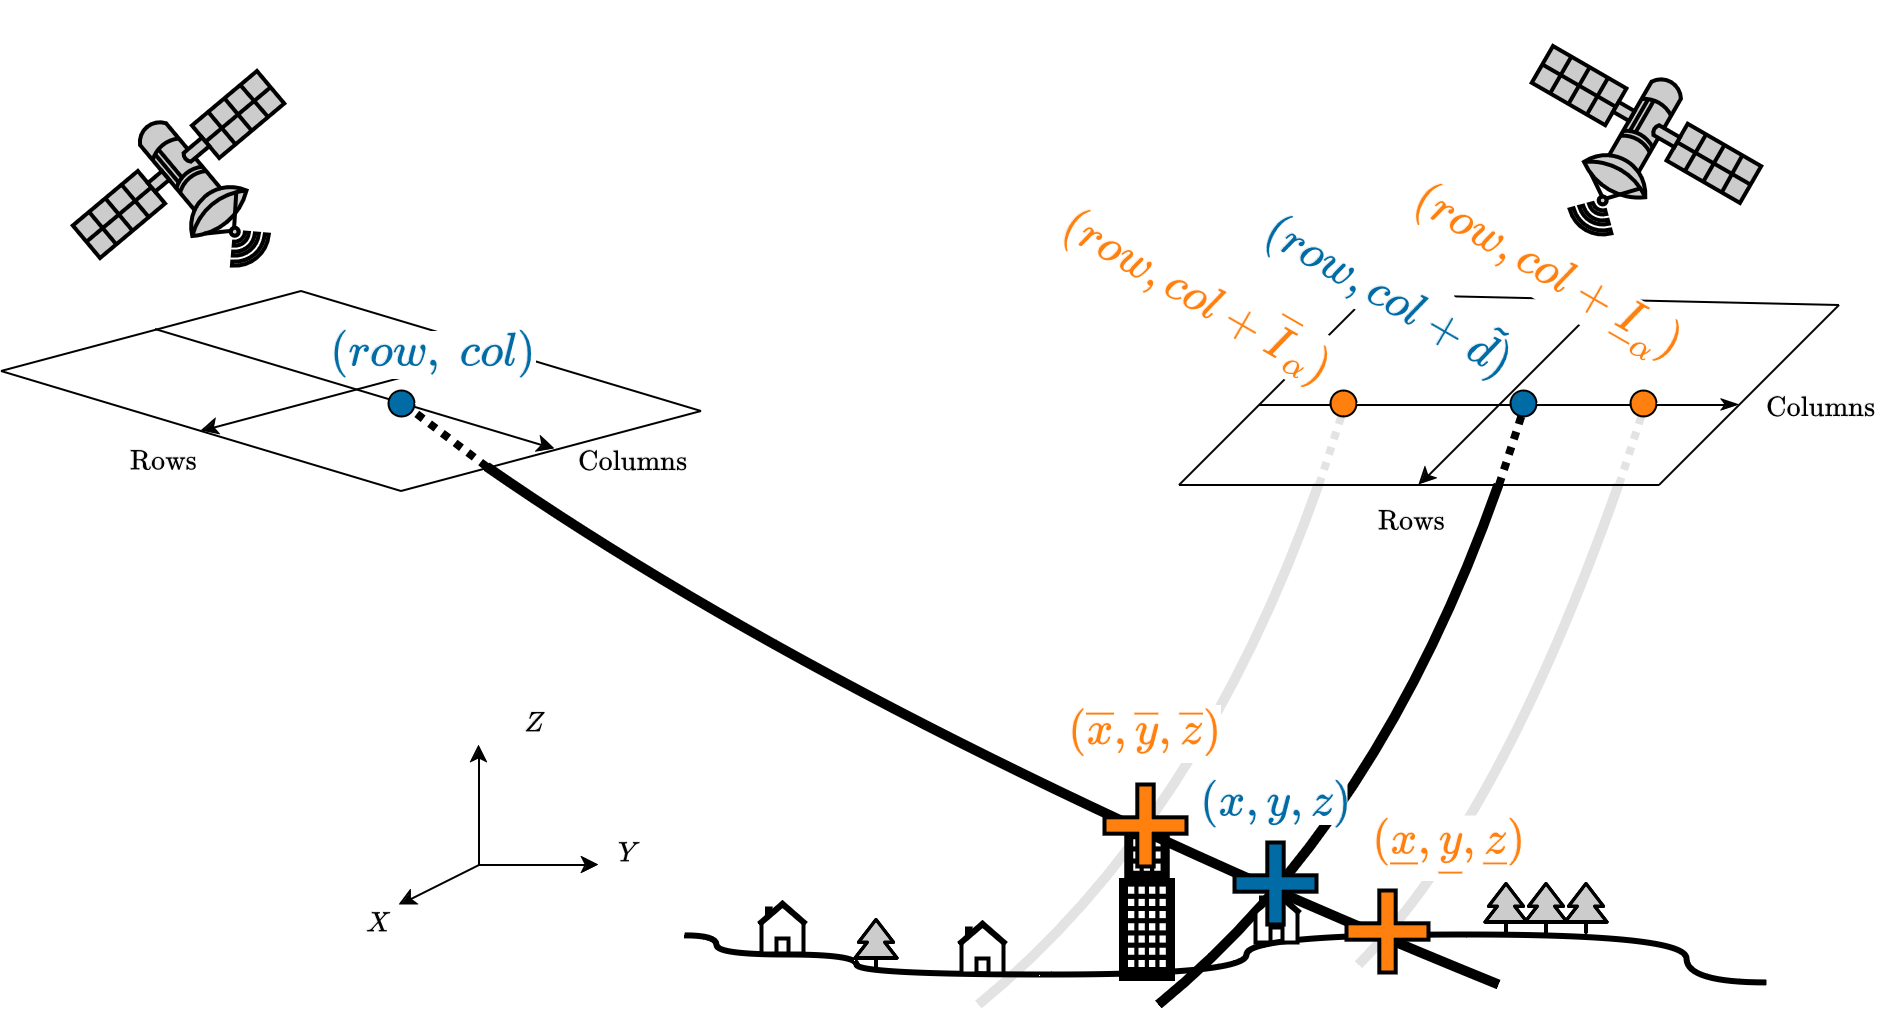
\includegraphics[width=\linewidth]{Images/Chap_6/Pairs_of_line_of_sight.png}
    \caption{Triangulation of the three pairs of line of sight. The angle between lines of sight is exaggerated for the purpose of this illustration.}
    \label{fig:pairs_of_line_of_sight}
\end{figure}

Depending on the disposition of satellites, as well as which image is selected as the reference image, it is both possible that $\overline{z}\leqslant z \leqslant \underline{z}$ or $\underline{z}\leqslant z \leqslant \overline{z}$. In the following, and for simplicity, we will consider that $\underline{z}\leqslant z \leqslant \overline{z}$. This is not constraining, as we can just change the notations to unsure this inequality holds. We therefore have a 3D confidence ``interval'', defined as every point from the reference line of sight between $(\underline{x}, ~\underline{y}, ~\underline{z})$ and $(\overline{x}, ~\overline{y}, ~\overline{z})$. For instance in \Cref{fig:pairs_of_line_of_sight}, the reference line of sight is the one originating from the left satellite, and the confidence ``interval'' is the portion of this line of sight between the two orange crosses. It is not an interval \textit{per se}, as \acrshort{rpc} are polynomials and not straight line, but they are approximated by straight line in the computations so the distinction is superfluous. 

The point cloud obtained from the triangulation of the disparity map is then filtered, as detailed in \Cref{sec:rasterization}\comloic{tu pointes la rasterisation mais le filtrage tu le présentes dans la triangulation par contre}. If a 3D point is filtered, then we naturally also filter its interval with it. 

The final step of the pipeline is the rasterization, as our objective is to produce height confidence intervals associated with every value contained in the \acrshort{dsm}. However, rasterizing intervals along lines of sight as it stands raises an issue: we are not guaranteed that the rasterized intervals will remain coherent with the final \acrshort{dsm} when projected on the regular grid. A solution to circumvent this issue is to consider that the planimetric shift $\Delta XY=\sqrt{(x-\underline{x})^2+(y-\underline{y})^2}$ is small in comparison to the altimetric shift $\Delta Z=\sqrt{(z-\underline{z})^2}$\comloic{ce serait bien d'avoir des valeurs quantitatives sur des scénarios classiques Pléiades ou CO3D puisque ce sont les deux missions que tu cites le plus souvent en préambule}, and that we can therefore neglect it. The lower and upper bounds can thus be aligned directly above and below the predicted 3D point $(x, ~y, ~z)$, and they thus become:
\begin{align}
    (\overline{x}, ~\overline{y}, ~\overline{z}) ~\rightarrow~ (x, ~y, ~\overline{z})\\
    (\underline{x}, ~\underline{y}, ~\underline{z}) ~\rightarrow~ (x, ~y, ~\underline{z})
\end{align}
\Cref{fig:planimetric_shift} illustrates this modification, where the orange points along the line of sight are shifted in the $(X,~Y)$ plane to be vertically aligned with $(x, ~y, ~z)$. 

$\Delta Z$ is proportional to the disparity to elevation ratio $r_{alt}$, \ie the elevation shift resulting from a shift of one disparity. This ratio is also a good indicator of the magnitude of errors on the final \acrshort{dsm}. This ratio will be used in \Cref{sec:metrics_elevation} to normalize the errors for different scenes.
\begin{remark}
    \todoroman{A mettre en annexe plutôt ?}\commanue{Moi je pense que tu peux le laisse et pas forcément le mettre dans une remarque. Ton hypsothèse est valide en fonction de l'angle d'acquisition. Tu peux dire que de toute façon on évite de trop dépointer car cela a un impact sur la résolution. Donc à part cas exceptionnel à vérifier quand on fait un vidéo mais pas plus à plus de 30°}\comloic{idem je le laisserai là et je pointerai les résultats dans la phrase plus haut sur laquelle en comm je te demandais déjà si on avait des résultats pour appuyer cette décision} The hypothesis that $\Delta XY$ is small compared to $\Delta Z$ depends only on the incidence angle $\beta$ of the reference image. Indeed, it holds that $\dfrac{\Delta Z}{\Delta XY}=\dfrac{1}{\tan(\beta)}$, where $\beta$ is the incidence angle as depicted in \Cref{fig:incidence_angle}. Ideally, if the reference image has no incidence angle, then the $\Delta XY$ shift is null. \Cref{tab:angle_coupling_pleiades} details the different incidence angles encountered in our experiments. The incidence angles are typically around $10\degree$, \ie $\Delta Z$ is around $5.6$ times bigger than $\Delta XY$. For the scene in Paris where the incidence reaches $6.1\degree$, the ratio is around $10$, while the only scene with $21.3\degree$, near Peyto Lake, Canada, has a ratio around $2.6$. For this last acquisition, the hypothesis that $\Delta XY$ is small compared to $\Delta Z$ is debatable, but we will still neglect $\Delta XY$ in the rasterization in order to stay consistent across our experiments. This will also allow to verify if this hypothesis can impact the performances of our method.
\end{remark}

\begin{figure}
    \centering
    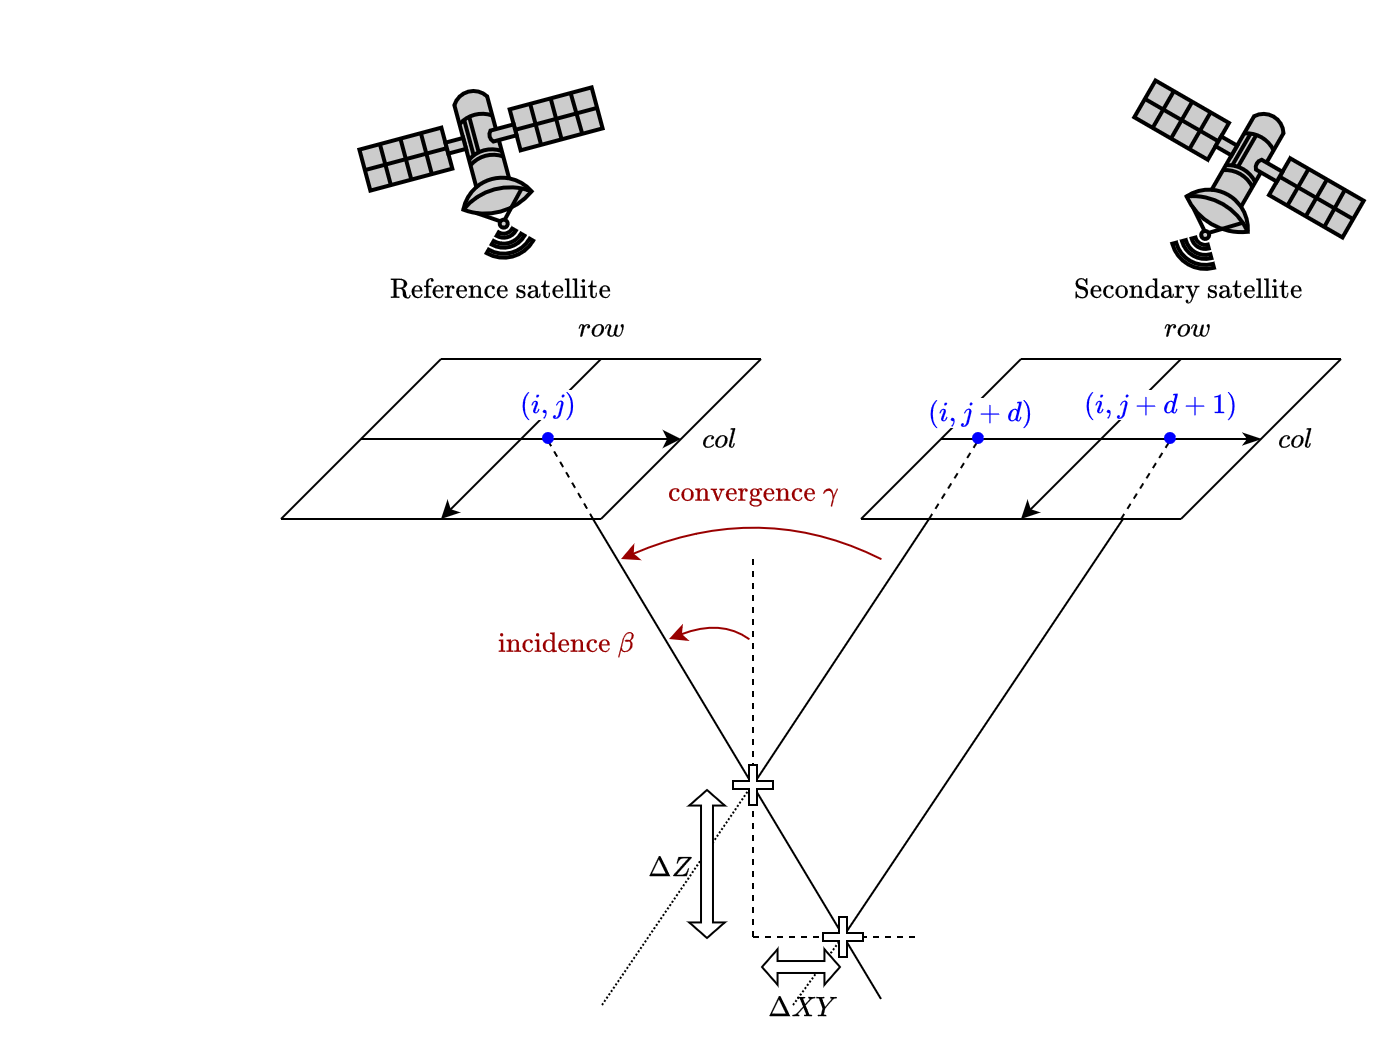
\includegraphics[width=0.8\linewidth]{Images/Chap_6/Incidence_angle.png}
    \caption{Acquisition angles of satellites}
    \label{fig:incidence_angle}
\end{figure}

\begin{figure}
    \centering
    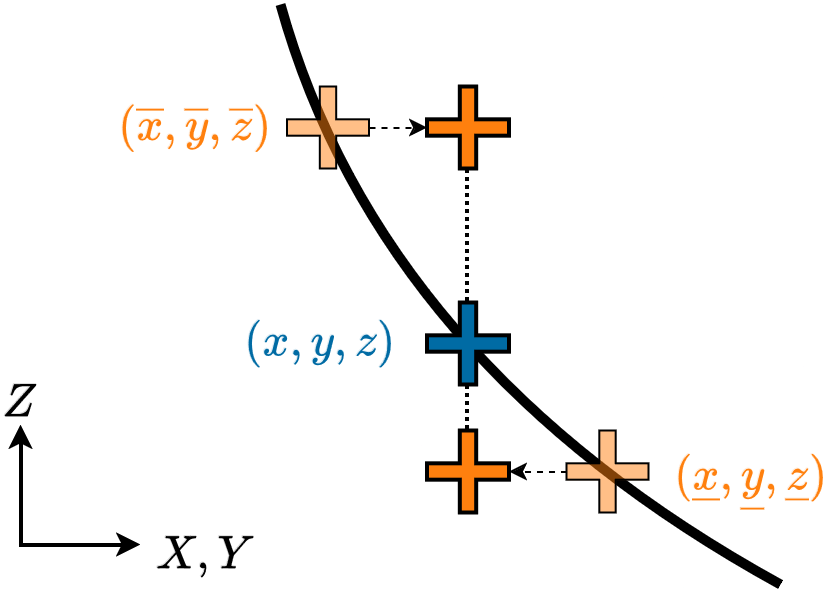
\includegraphics[width=0.6\linewidth]{Images/Chap_6/Planimetric_shift.png}
    \caption{Aligning the confidence interval bounds along a line of sight}
    \label{fig:planimetric_shift}
\end{figure}

We remind here the general formulation of the rasterization step\commanue{peut-être que je mettrais des sous-sous-sections histoire de faire apparaître les différentes étapes de CARS que tu considères}\comloic{j'irai bien dans le sens de Manue ici}, where each cell $(x,~y)$ of the \acrshort{dsm} is computed using a weighted mean on its neighboring $\N(x,y)$ :
\begin{align}
    \DSM(x,y) &= \dfrac{\sum\limits_{(x_i, y_i, z_i)\in\N(x,y)}z_i\cdot w(x_i, y_i)}{\sum\limits_{(x_i,y_i,z_i)\in\N(x,y)} w(x_i, y_i)}
\end{align}
where weights $w(x_i,y_i)$ are positive scalars. In CARS, they are computed using a Gaussian distribution, but other pipelines also use Inverse Distance Weightings which works similarly. Because it holds that for any point, $\underline{z}\leqslant z\leqslant\overline{z}$, then computing the \acrshort{dsm}s independently using $(x, ~y, ~z)$, $(x, ~y, ~\overline{z})$ and $(x, ~y, ~\underline{z})$ will ensure the consistency of resulting \acrshort{dsm}s:
\begin{eqnarray}
    \dfrac{\sum\limits_{(x_i, y_i, \underline{z}_i)\in\N(x,y)}\underline{z}_i\cdot w(x_i, y_i)}{\sum\limits_{(x_i,y_i, \underline{z}_i)\in\N(x,y)} w(x_i, y_i)}
    \leqslant&
    \dfrac{\sum\limits_{(x_i, y_i, z_i)\in\N(x,y)}z_i\cdot w(x_i, y_i)}{\sum\limits_{(x_i,y_i,z_i)\in\N(x,y)} w(x_i, y_i)}
    &\leqslant
    \dfrac{\sum\limits_{(x_i, y_i, \overline{z}_i)\in\N(x,y)}\overline{z}_i\cdot w(x_i, y_i)}{\sum\limits_{(x_i,y_i,\overline{z}_i)\in\N(x,y)} w(x_i, y_i)}\nonumber\\
    &&\nonumber\\
    \underline{\DSM}(x,y) \leqslant& \DSM(x,y) &\leqslant\overline{DSM}(x,y)
\end{eqnarray}
where $\underline{\DSM}(x,y)$ is the \acrshort{dsm} computed using points $(x, ~y, ~\underline{z})$, and $\overline{\DSM}(x,y)$ is the \acrshort{dsm} computed using points $(x, ~y, ~\overline{z})$. For each value of the \acrshort{dsm} $\DSM(x,y)$ we have now computed a height interval $[\underline{\DSM}(x,y),~\overline{\DSM}(x,y)]$. We will make no distinction between height intervals and elevation intervals in the following. 

As rasterization is the final step of the stereo pipeline, we now have propagated the confidence intervals all the way to the end of the pipeline while insuring their coherency with the predicted \acrshort{dsm} and without influencing the values of the final \acrshort{dsm}. The next step is therefore to evaluate the confidence height intervals on real data to verify if the potential errors occurring during the transformation of disparity intervals into elevation intervals do not question their accuracy.

\section{Acquiring and Processing Data for Evaluation}
\subsection{Satellite and DSM datasets}\commanue{Petit retour en arrière, je me rends compte que tu ne mentionnes jamais l'intervalle de recherche de la disparité. L'objectif est aussi de montrer que ta méthode ne donne des intervalles aussi larges que l'intervalle de recherche.}
This section will present the different images and ground truth \acrshort{dsm}s used to evaluate elevation intervals. There are two sources for ground truth \acrshort{dsm}s. The first source are\comloic{j'ai un petit doute sur le "the first source are DSMs", tu es sur que c'est correct comme formulation ?} \acrshort{dsm}s over mountainous regions containing glaciers. They have been kindly provided by Etienne Berthier from LEGOS, Liss Marie Andreassen from the Norwegian Water Resources and Energy Directorate (NVE) and Brian Menounos from the Natural Sciences and Engineering Research Council of Canada and the Tula Foundation (Hakai Institute). The data were acquired in the following regions:
\begin{itemize}
    \item Mountains near Peyto lake, in the Alberta province of Canada. (\Cref{fig:miniature_Peyto})
    \item Two different \acrshort{dsm}s in the mountainous region of Jotunheinem, Norway. We will refer to each \acrshort{dsm} as Hellmem (\Cref{fig:miniature_Hellmem}) and Graasubreen (\Cref{fig:miniature_Graasubreen}).
    \item Langfjordjøkelen glacier, Norway (\Cref{fig:miniature_Langfjordjokelen}).
\end{itemize}
The ground truth were acquired by \acrshort{lidar} data, rasterized at 50cm resolution. We did not applied the rasterization ourselves and only had access to the rasterized \acrshort{dsm}. The second source of ground truth data comes from the \acrshort{lidar} HD program (\cite{monnet_lidarhd_2023} \url{https://geoservices.ign.fr/lidarhd}) which intends to cover the whole french territory (except French Guiana) by the end of 2026. It is a very rich source of information, with around $10$ measured points per m$^2$ and a planimetric precision of 50cm. As of the time we write this thesis, not all regions of France are publicly available. From the data available at the time\comloic{le temps des travaux ou le temps de la rédaction?}, we selected different regions of interest in order to have a variety of landscapes (rural, urban, seaside \etc). Those landscapes all presented strong elevation variations in order to present a challenge for the stereo pipeline. We also want to determine if our method behaves differently depending on the nature of the scene. Here is the list of the considered regions:
\begin{itemize}
    \item The city of Bordeaux (\Cref{fig:miniature_Bordeaux})
    \item The city of Paris (\Cref{fig:miniature_Paris})
    \item The city of Montpellier (\Cref{fig:miniature_Montpellier})
    \item The city of Toulouse (\Cref{fig:miniature_Toulouse})
    \item Mediterranean coastline with the city of Monaco (\Cref{fig:miniature_Monaco})
    \item Valleys and mountains near Grenoble, in the french Alps (\Cref{fig:miniature_Grenoble})
    \item Valleys and mountains at Pic du Midi, french Pyrenees (\Cref{fig:miniature_pic_du_midi})
\end{itemize}
The \acrshort{lidar} point clouds were then rasterized at 50cm resolution with the same Gaussian rasterization method as in the stereo pipeline. \Cref{tab:dates_pleiades_lidar_hd} presents the different acquisition dates and shape of the ground truth \acrshort{dsm}.

We used Pléiades images for producing both \acrshort{dsm}s and intervals that will be compared to the ground truth. We did not directly ordered the Pléiades acquisitions, as it is costly and hard to synchronise with the acquisition date of the ground truth. From the available catalogue, we selected stereo pairs that were acquired as close as possible from the acquisition date of the ground truth, or if multiple months separated the two acquisitions, we rather selected a similar period of previous/next year to minimize seasonal changes. \Cref{tab:dates_pleiades_lidar_hd} allows to compare dates of acquisition of the \acrshort{lidar} and Pléiades images.

We saw in \Cref{sec:elevation_intervals} that the planimetric and altimetric resolution (and errors) were defined by the incidence and convergence angles of the lines of sights of the satellites\commanue{the planimetric and altimetric accuracy depend on the incidence and convergence angles of the lines of sights of the satellites?}. \Cref{tab:angle_coupling_pleiades} presents those angles for the different Pléiades images.

\begin{table}[ht]
    \centering
    \begin{tabular}{|c||c|c|c|}
    \hline
        Area & Date for LiDAR & Date of Pléiades &  GT Size (0.5m)\\
        \hline\hline
        Bordeaux & 2023-09-15 & 2022-08-04 & $6001\times 6001$\\\hline
        Grenoble & 2021-09-05 & 2020-09-17 & $10 001\times 10 001$ \\\hline
        Hellmem 1 & 2019-08-27 & 2019-08-27 & $7127\times 7298$ \\\hline
        Graasubreen 2 & 2019-08-27 & 2019-08-27 & $3912\times2880$ \\\hline
        Langfjordjøkelen & 2018-09-01 & 2018-09-01 & $5841\times 3689$\\\hline
        Monaco & 2021-05-13 & 2020-08-30 & $10 001\times 10 001$\\\hline
        Montpellier & 2021-05-28 & 2021-10-17 & $8001\times 8001$\\\hline
        Paris & 2023-03-03 & 2023-05-31 & $10 001\times 10 001$\\\hline
        Peyto & 2016-09-13 & 2016-09-13 & $13240\times 17874$\\\hline
        Pic du Midi & 2021-10-02 & 2021-10-16 & $10001 \times 12001$ \\\hline
        Toulouse & 2022-05-29 & 2022-06-28 & $12001\times 8001$\\\hline
    \end{tabular}
    \caption{Acquisition date of Pléiade stereo or tri-stereo images, and the \acrshort{lidar} ground truth}
    \label{tab:dates_pleiades_lidar_hd}
\end{table}

\begin{table}[ht]
    \centering
    \begin{tabular}{|c||c|c|c|c|}
        \hline
        Area & Convergence & Incidence left & Incidence right \\
        \hline\hline
        Bordeaux & 23.1\degree & 9.7\degree & 14.2\degree \\\hline
        Grenoble & 28.3\degree & 12.4\degree & 16.1\degree \\\hline
        Jotunheinem & 22.5\degree & 10.6\degree & 14.5\degree \\\hline
        Langfjordjøkelen & 21.4\degree & 10.2\degree & 13.8\degree \\\hline
        Monaco & 29.2\degree & 12.8\degree & 18.1\degree \\\hline
        Montpellier & 7.7\degree & 11.5\degree & 15\degree\\\hline
        Paris & 4.9\degree& 6.1\degree & 7.9\degree\\\hline
        Peyto & 17.2\degree & 21.3\degree & 21.6\degree \\\hline
        Pic du Midi & 29.0\degree & 13.7\degree & 15.3\degree \\\hline
        Toulouse & 11.4\degree & 12.5\degree & 18.7\degree\\\hline
    \end{tabular}
    \caption{Relevant angles of stereo pairs of Pléiades images. See \Cref{fig:incidence_angle} for a schematic representation of those angles.}
    \label{tab:angle_coupling_pleiades}
\end{table}
\commanue{vu que tu as de la place je mettrais convergence angle, left incidence angle, right incidence angle}

\begin{figure}
    \centering
    \begin{subfigure}[t]{0.48\linewidth}
        \flushleft
        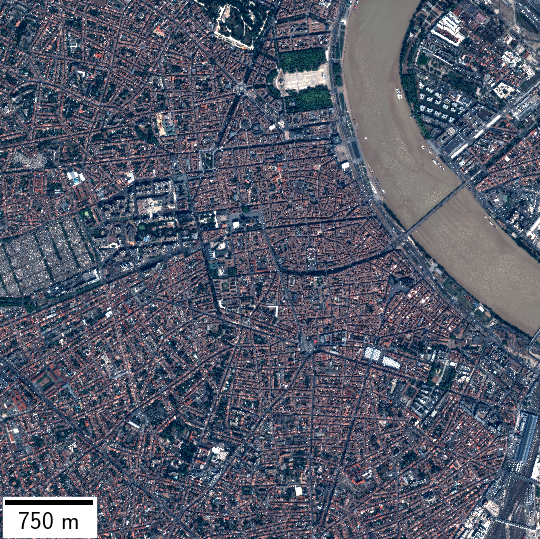
\includegraphics[width=\linewidth]{Images/Chap_6/miniature_Bordeaux.png}
        \caption{\acrshort{rgb} image of Bordeaux (Pléiades © CNES 2022, Distribution AIRBUS DS)}
        \label{fig:miniature_Bordeaux_rgb}
    \end{subfigure}\hfill
    \begin{subfigure}[t]{0.48\linewidth}
        \flushright
        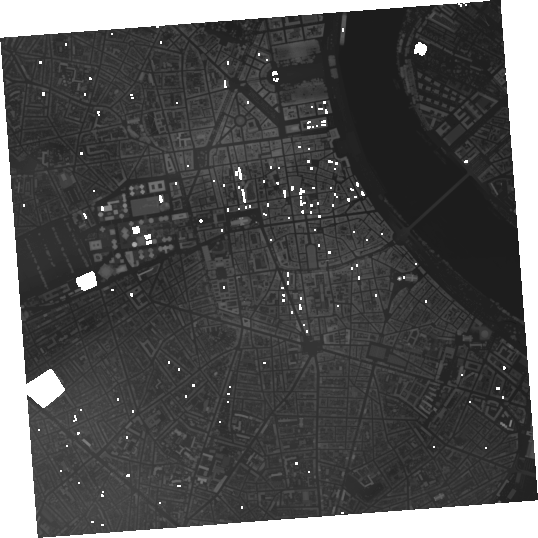
\includegraphics[width=\linewidth]{Images/Chap_6/miniature_Bordeaux_gt.png}
        \caption{\acrshort{lidar} HD \acrshort{dsm}}
        \label{fig:miniature_Bordeaux_gt}
    \end{subfigure}
    \caption{\acrshort{rgb} image of Bordeaux and its associated ground truth \acrshort{dsm}.}
    \label{fig:miniature_Bordeaux}
\end{figure}

\begin{figure}
    \centering
    \begin{subfigure}[t]{0.48\linewidth}
        \flushleft
        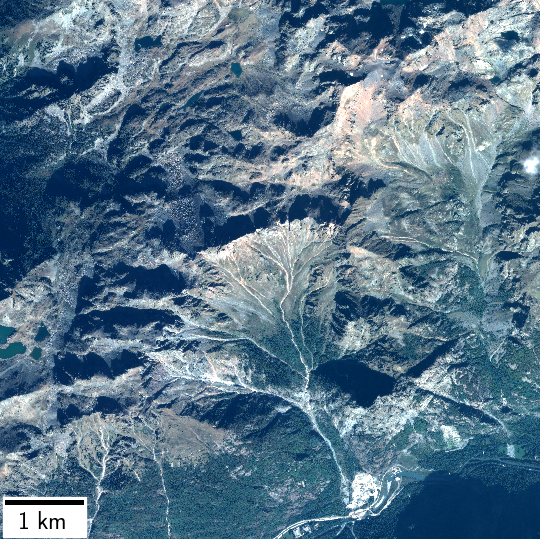
\includegraphics[width=\linewidth]{Images/Chap_6/miniature_Grenoble.png}
        \caption{\acrshort{rgb} image of a region near Grenoble (Pléiades © CNES 2020, Distribution AIRBUS DS)}
        \label{fig:miniature_Grenoble_rgb}
    \end{subfigure}\hfill
    \begin{subfigure}[t]{0.48\linewidth}
        \flushright
        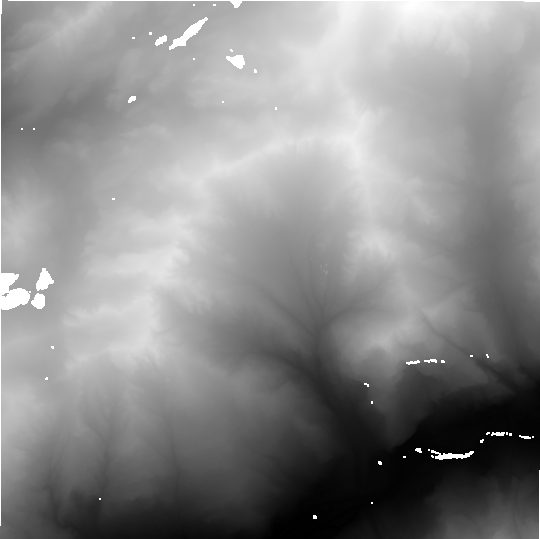
\includegraphics[width=\linewidth]{Images/Chap_6/miniature_Grenoble_gt.png}
        \caption{\acrshort{lidar} HD \acrshort{dsm}}
        \label{fig:miniature_Grenoble_gt}
    \end{subfigure}
    \caption{\acrshort{rgb} image of Grenoble and its associated ground truth \acrshort{dsm}.}
    \label{fig:miniature_Grenoble}
\end{figure}

\begin{figure}
    \centering
    \begin{subfigure}[t]{0.48\linewidth}
        \flushleft
        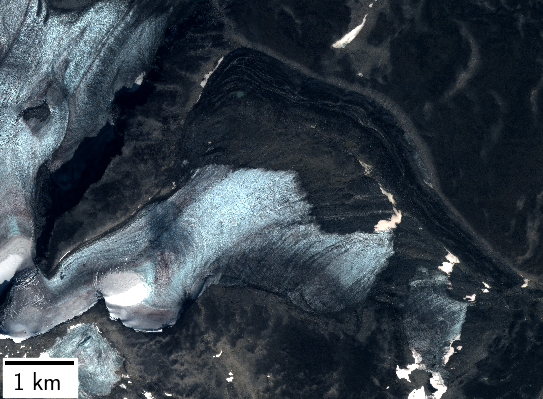
\includegraphics[width=\linewidth]{Images/Chap_6/miniature_Graasubreen.png}
        \caption{\acrshort{rgb} image of Graasubreen (Pléiades © CNES 2019, Distribution AIRBUS DS)}
        \label{fig:miniature_Graasubreen_rgb}
    \end{subfigure}\hfill
    \begin{subfigure}[t]{0.48\linewidth}
        \flushright
        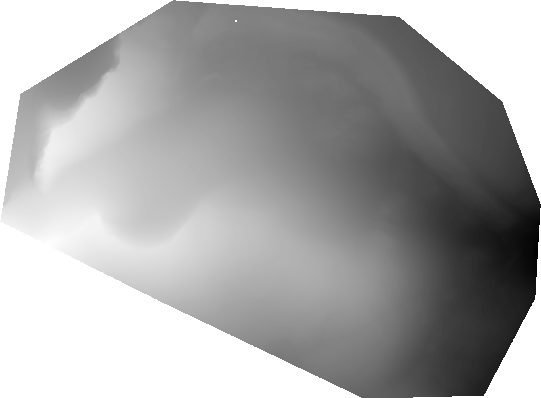
\includegraphics[width=\linewidth]{Images/Chap_6/miniature_Graasubreen_gt.png}
        \caption{\acrshort{lidar} \acrshort{dsm}}
        \label{fig:miniature_Graasubreen_gt}
    \end{subfigure}
    \caption{\acrshort{rgb} image of Graasubreen and its associated ground truth \acrshort{dsm}.}
    \label{fig:miniature_Graasubreen}
\end{figure}

\begin{figure}
    \centering
    \begin{subfigure}[t]{0.48\linewidth}
        \flushleft
        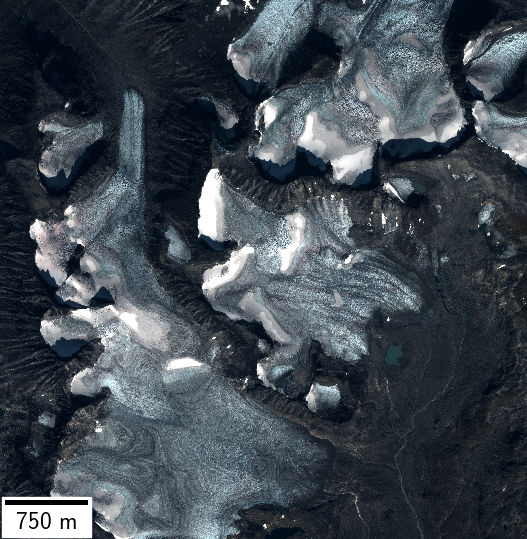
\includegraphics[width=\linewidth]{Images/Chap_6/miniature_Hellmem.png}
        \caption{\acrshort{rgb} image of Hellmem (Pléiades © CNES 2019, Distribution AIRBUS DS)}
        \label{fig:miniature_Hellmem_rgb}
    \end{subfigure}\hfill
    \begin{subfigure}[t]{0.48\linewidth}
        \flushright
        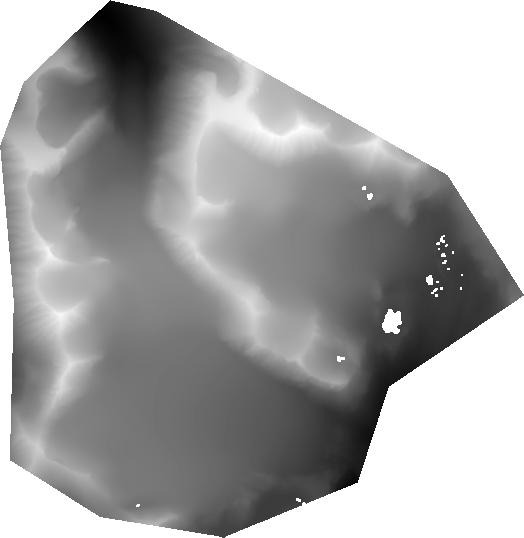
\includegraphics[width=\linewidth]{Images/Chap_6/miniature_Hellmem_gt.png}
        \caption{\acrshort{lidar} \acrshort{dsm}}
        \label{fig:miniature_Hellmem_gt}
    \end{subfigure}
    \caption{\acrshort{rgb} image of Hellmem and its associated ground truth \acrshort{dsm}.}
    \label{fig:miniature_Hellmem}
\end{figure}

\begin{figure}
    \centering
    \begin{subfigure}[t]{0.48\linewidth}
        \flushleft
        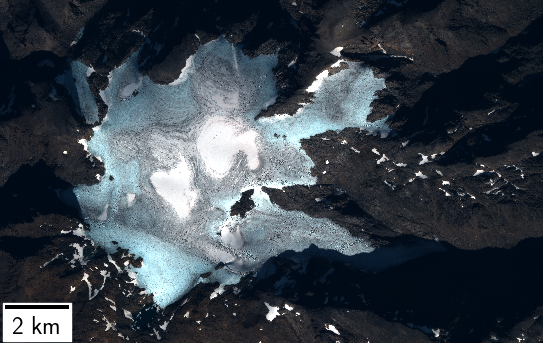
\includegraphics[width=\linewidth]{Images/Chap_6/miniature_Langfjordjokelen.png}
        \caption{\acrshort{rgb} image of Langfjordjøkelen (Pléiades © CNES 2018, Distribution AIRBUS DS)}
        \label{fig:miniature_Langfjordjokelen_rgb}
    \end{subfigure}\hfill
    \begin{subfigure}[t]{0.48\linewidth}
        \flushright
        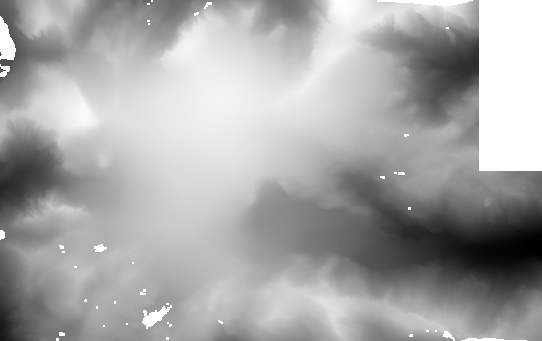
\includegraphics[width=\linewidth]{Images/Chap_6/miniature_Langfjordjokelen_gt.png}
        \caption{\acrshort{lidar} \acrshort{dsm}}
        \label{fig:miniature_Langfjordjokelen_gt}
    \end{subfigure}
    \caption{\acrshort{rgb} image of Langfjordjøkelen and its associated ground truth \acrshort{dsm}.}
    \label{fig:miniature_Langfjordjokelen}
\end{figure}

\begin{figure}
    \centering
    \begin{subfigure}[t]{0.48\linewidth}
        \flushleft
        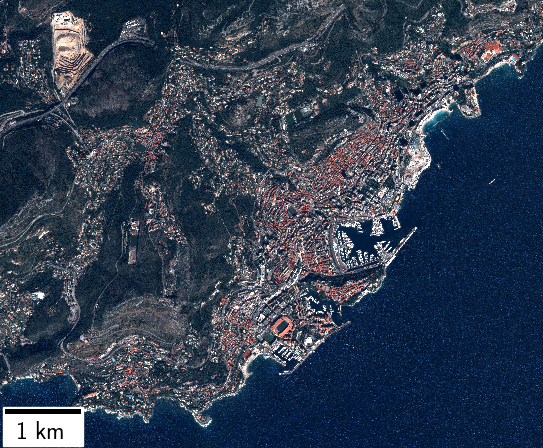
\includegraphics[width=\linewidth]{Images/Chap_6/miniature_Monaco.png}
        \caption{\acrshort{rgb} image of Monaco (Pléiades © CNES 2020, Distribution AIRBUS DS)}
        \label{fig:miniature_Monaco_rgb}
    \end{subfigure}\hfill
    \begin{subfigure}[t]{0.48\linewidth}
        \flushright
        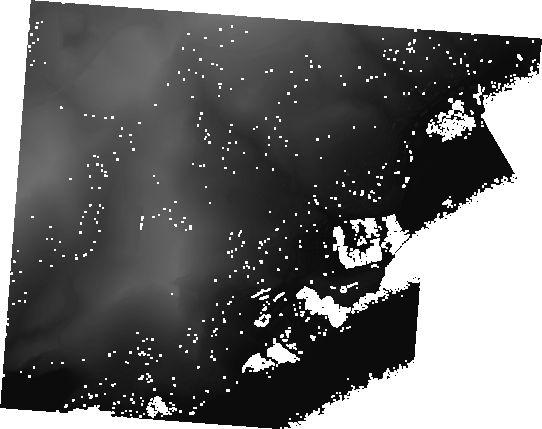
\includegraphics[width=\linewidth]{Images/Chap_6/miniature_Monaco_gt.png}
        \caption{\acrshort{lidar} HD \acrshort{dsm}}
        \label{fig:miniature_Monaco_gt}
    \end{subfigure}
    \caption{\acrshort{rgb} image of Monaco and its associated ground truth \acrshort{dsm}.}
    \label{fig:miniature_Monaco}
\end{figure}

\begin{figure}
    \centering
    \begin{subfigure}[t]{0.48\linewidth}
        \flushleft
        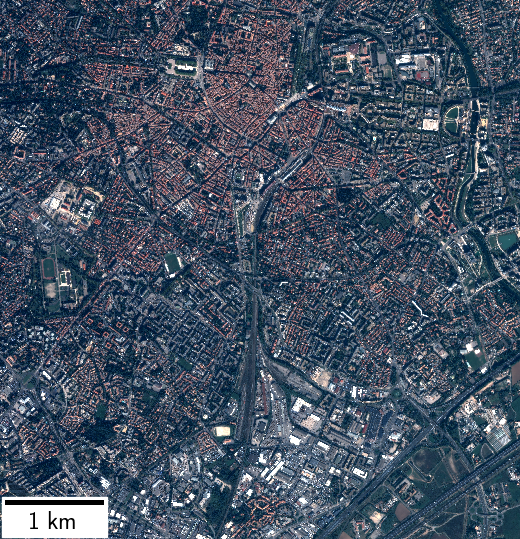
\includegraphics[width=\linewidth]{Images/Chap_6/miniature_Montpellier.png}
        \caption{\acrshort{rgb} image of Montpellier (Pléiades © CNES 2020, Distribution AIRBUS DS)}
        \label{fig:miniature_Montpellier_rgb}
    \end{subfigure}\hfill
    \begin{subfigure}[t]{0.48\linewidth}
        \flushright
        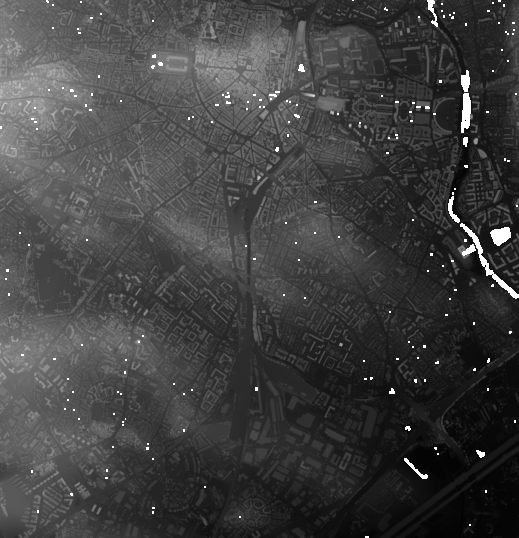
\includegraphics[width=\linewidth]{Images/Chap_6/miniature_Montpellier_gt.png}
        \caption{\acrshort{lidar} HD \acrshort{dsm}}
        \label{fig:miniature_Montpellier_gt}
    \end{subfigure}
    \caption{\acrshort{rgb} image of Montpellier and its associated ground truth \acrshort{dsm}.}
    \label{fig:miniature_Montpellier}
\end{figure}

\begin{figure}
    \centering
    \begin{subfigure}[t]{0.48\linewidth}
        \flushleft
        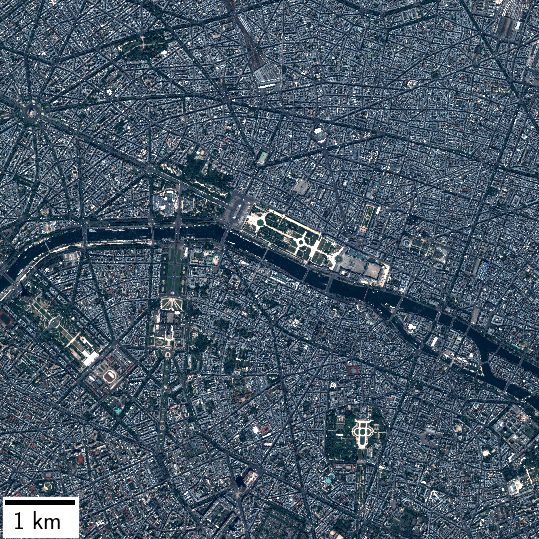
\includegraphics[width=\linewidth]{Images/Chap_6/miniature_Paris.png}
        \caption{\acrshort{rgb} image of Paris (Pléiades © CNES 2023, Distribution AIRBUS DS)}
        \label{fig:miniature_Paris_rgb}
    \end{subfigure}\hfill
    \begin{subfigure}[t]{0.48\linewidth}
        \flushright
        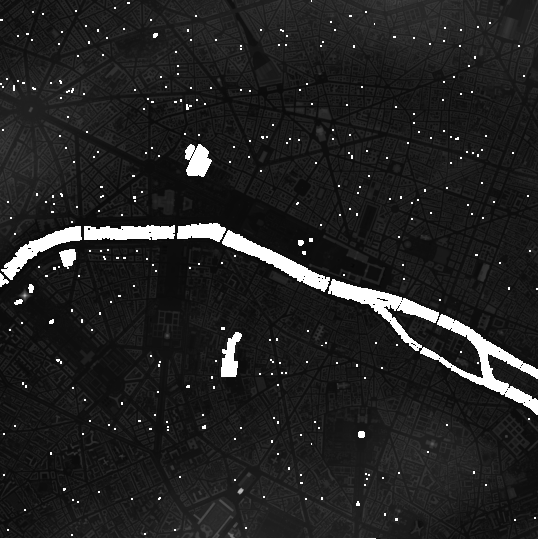
\includegraphics[width=\linewidth]{Images/Chap_6/miniature_Paris_gt.png}
        \caption{\acrshort{lidar} HD \acrshort{dsm}}
        \label{fig:miniature_Paris_gt}
    \end{subfigure}
    \caption{\acrshort{rgb} image of  and its associated ground truth \acrshort{dsm}.}
    \label{fig:miniature_Paris}
\end{figure}

\begin{figure}
    \centering
    \begin{subfigure}[t]{0.48\linewidth}
        \flushleft
        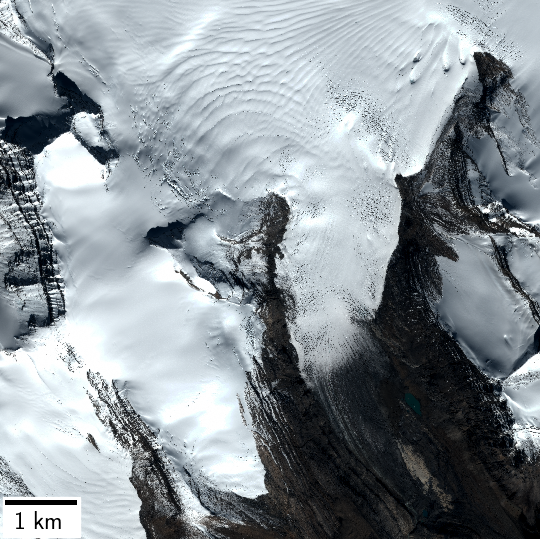
\includegraphics[width=\linewidth]{Images/Chap_6/miniature_Peyto.png}
        \caption{\acrshort{rgb} image of Peyto (Pléiades © CNES 2016, Distribution AIRBUS DS)}
        \label{fig:miniature_Peyto_rgb}
    \end{subfigure}\hfill
    \begin{subfigure}[t]{0.48\linewidth}
        \flushright
        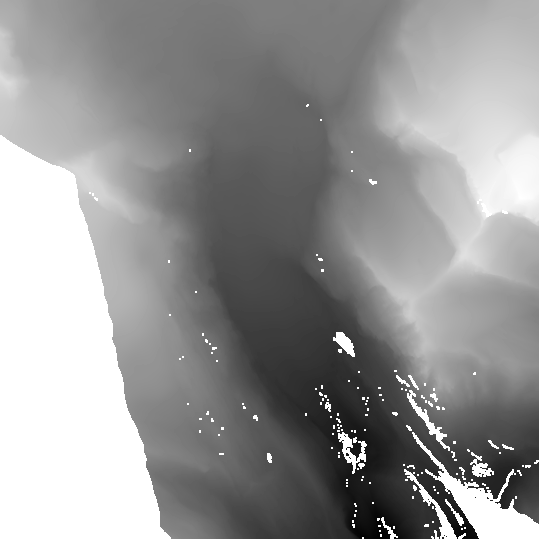
\includegraphics[width=\linewidth]{Images/Chap_6/miniature_Peyto_gt.png}
        \caption{\acrshort{lidar} HD \acrshort{dsm}}
        \label{fig:miniature_Peyto_gt}
    \end{subfigure}
    \caption{\acrshort{rgb} image of Peyto and its associated ground truth \acrshort{dsm}.}
    \label{fig:miniature_Peyto}
\end{figure}

\begin{figure}
    \centering
    \begin{subfigure}[t]{0.48\linewidth}
        \flushleft
        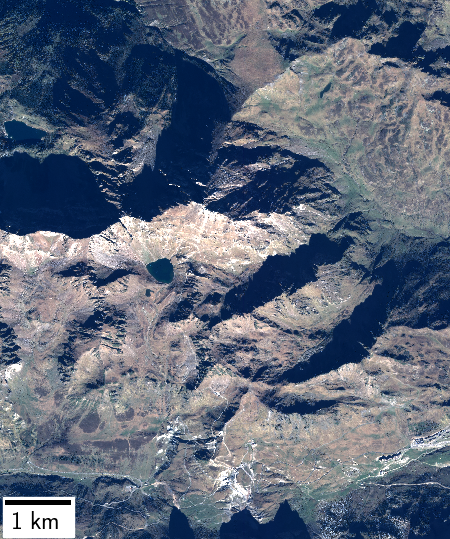
\includegraphics[width=\linewidth]{Images/Chap_6/miniature_Pic_du_midi.png}
        \caption{\acrshort{rgb} image of Pic du Midi (Pléiades © CNES 2021, Distribution AIRBUS DS)}
        \label{fig:miniature_pic_du_midi_rgb}
    \end{subfigure}\hfill
    \begin{subfigure}[t]{0.48\linewidth}
        \flushright
        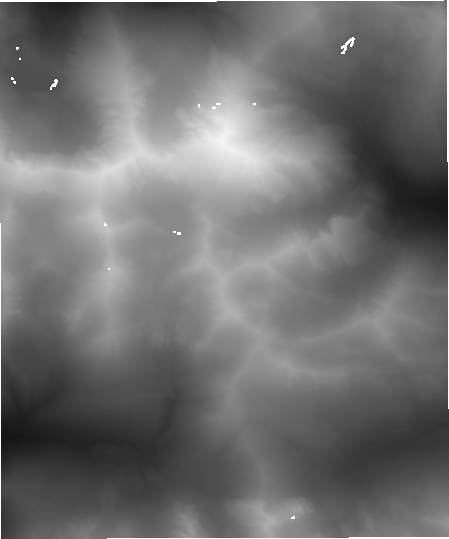
\includegraphics[width=\linewidth]{Images/Chap_6/miniature_Pic_du_midi_gt.png}
        \caption{\acrshort{lidar} HD \acrshort{dsm}}
        \label{fig:miniature_pic_du_midi_gt}
    \end{subfigure}
    \caption{\acrshort{rgb} image of Pic du Midi and its associated ground truth \acrshort{dsm}.}
    \label{fig:miniature_pic_du_midi}
\end{figure}

\begin{figure}
    \centering
    \begin{subfigure}[t]{0.48\linewidth}
        \flushleft
        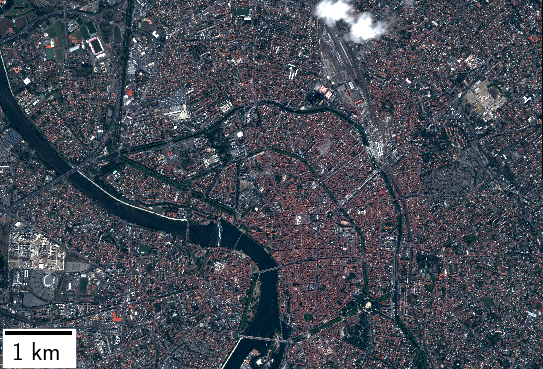
\includegraphics[width=\linewidth]{Images/Chap_6/miniature_Toulouse.png}
        \caption{\acrshort{rgb} image of Toulouse (Pléiades © CNES 2022, Distribution AIRBUS DS)}
        \label{fig:miniature_Toulouse_rgb}
    \end{subfigure}\hfill
    \begin{subfigure}[t]{0.48\linewidth}
        \flushright
        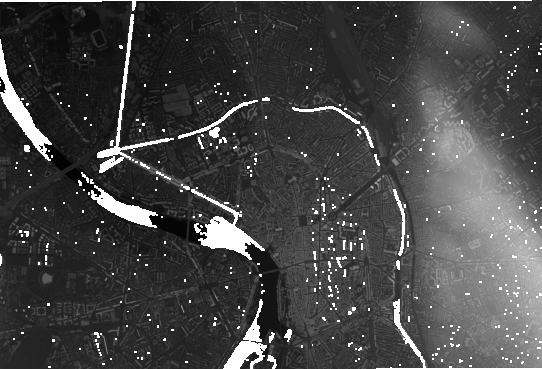
\includegraphics[width=\linewidth]{Images/Chap_6/miniature_Toulouse_gt.png}
        \caption{\acrshort{lidar} HD \acrshort{dsm}}
        \label{fig:miniature_Toulouse_gt}
    \end{subfigure}
    \caption{\acrshort{rgb} image of Toulouse and its associated ground truth \acrshort{dsm}.}
    \label{fig:miniature_Toulouse}
\end{figure}

\subsection{Water Masks}
Both \acrshort{lidar} data and stereo correlation present poor results on water surfaces. For the \acrshort{lidar} data, wavelengths are often absorbed by still water and do not provide the sensor with any feedback (although turbid water can usually send back some signal). For moving waters, the provided signal is often noisy and needs post processing to remove artifacts. Stereophotogrammetry has usual even poorer results, because open waters are texture-less or uniform surfaces on which the correlation does not perform well. Furthermore, for Pléiades acquisitions, the water has moved\commanue{may have moved?} between images which prevents water pixels to be correctly triangulated. For those reasons, we chose to add a water mask on images of cities crossed by a river (Bordeaux, Monaco, Montpellier, Paris and Toulouse) or near the seaside (Monaco). The water mask was obtained using an algorithm developed by CNES, which uses a random forest trained on existing high resolution mapping of surface waters \cite{pekel_high-resolution_2016} and the Normalized Difference Water Index \cite{gao_ndwinormalized_1996}. \Cref{fig:paris_watermask_2} presents a water mask produced on the image of Paris.

\begin{figure}
    \centering
    \begin{subfigure}[t]{0.48\linewidth}
        \flushleft
        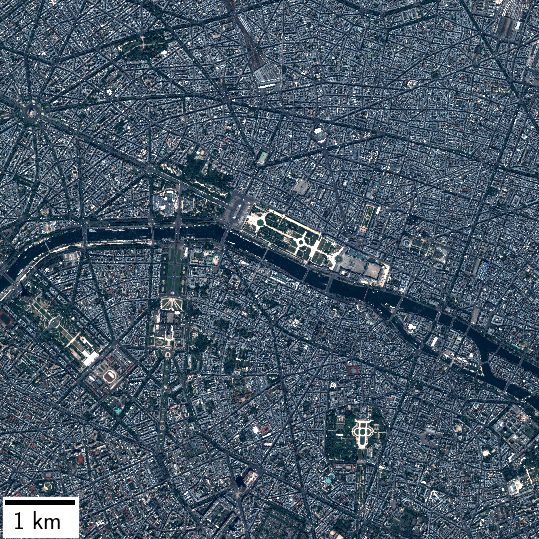
\includegraphics[width=\linewidth]{Images/Chap_6/miniature_Paris.png}
        \caption{\acrshort{rgb} image of Paris (Pléiades © CNES 2023, Distribution AIRBUS DS)}
        \label{fig:paris_watermask_1}
    \end{subfigure}\hfill
    \begin{subfigure}[t]{0.48\linewidth}
        \flushright
        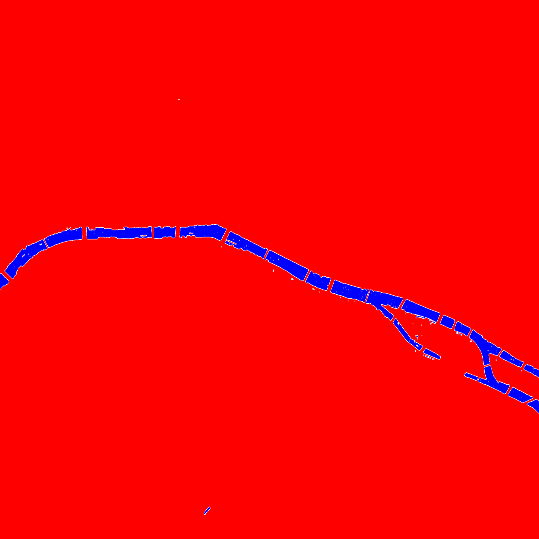
\includegraphics[width=\linewidth]{Images/Chap_6/watermask_Paris.png}
        \caption{Water mask}
        \label{fig:paris_watermask_2}
    \end{subfigure}
    \caption{\acrshort{rgb} image of Paris and its associated water mask. Water is indicated by blue pixels}
    \label{fig:paris_watermask}
\end{figure}

\subsection{Co-registration}
The \acrshort{dsm}s obtained from \acrshort{lidar} data and from stereophotogrammetry are not necessarily in the same projection reference system, and do not use the same altitude reference. Moreover, due to the limited precision of the \acrshort{rpc} models and GPS measures of the \acrshort{lidar}, some planimetric and elevation bias may exist between the two \acrshort{dsm}s which do not allow their comparison as such. We therefore reproject the ground truth data in the same reference system as their corresponding \acrshort{dsm} produced by the CARS pipeline. We then rectify the planimetric and altimetric biases by employing the method presented in \cite{nuth_co-registration_2011}. This process is called co-registration\comloic{a vérifier, c'est peut être un abus de la langage, si tu l'as trouvé comme ça dans la littérature c'est top, si c'est une expression d'usage à Toulouse faudrait vérifier on a vite fait de trainer des expressions entre nous qui ne soient pas toujours exactes}. We quickly present the method for estimating the altimetric and planimetric biases, and refer to the original publication for additional details.

It is possible to observe that the measured differences between two shifted \acrshort{dsm}s vary with the slope angle and the orientation of the slope. The different parameters influencing the measured variations of elevation, presented in \Cref{fig:coregistration}, are the following:
\begin{itemize}
    \item We note $\sigma$ the angle of a slope. $\sigma=0\degree$ corresponds to a flat slope and $\sigma=90\degree$ to a vertical slope.
    \item We note $\psi$ the azimuth of the slope. If the slope faces north, then $\psi=0\degree$. If it faces west, $\psi=90\degree$ \etc
    \item The direction of the planimetric shift between \acrshort{dsm}s is given by an angle $\beta$, with the same conventions as the azimuth. The magnitude of the shift is $B$.
    \item $dh$ refers to measured local variations of elevation, and $\tilde{dh}$ is the global elevation shift between \acrshort{dsm}s.
\end{itemize}
The relation linking all those parameters is the following \cite{nuth_co-registration_2011}:
\begin{align}
    dh = B\cos(\psi-\beta)\tan(\sigma)+\tilde{dh}
\end{align}

\begin{figure}[ht!]
    \centering
    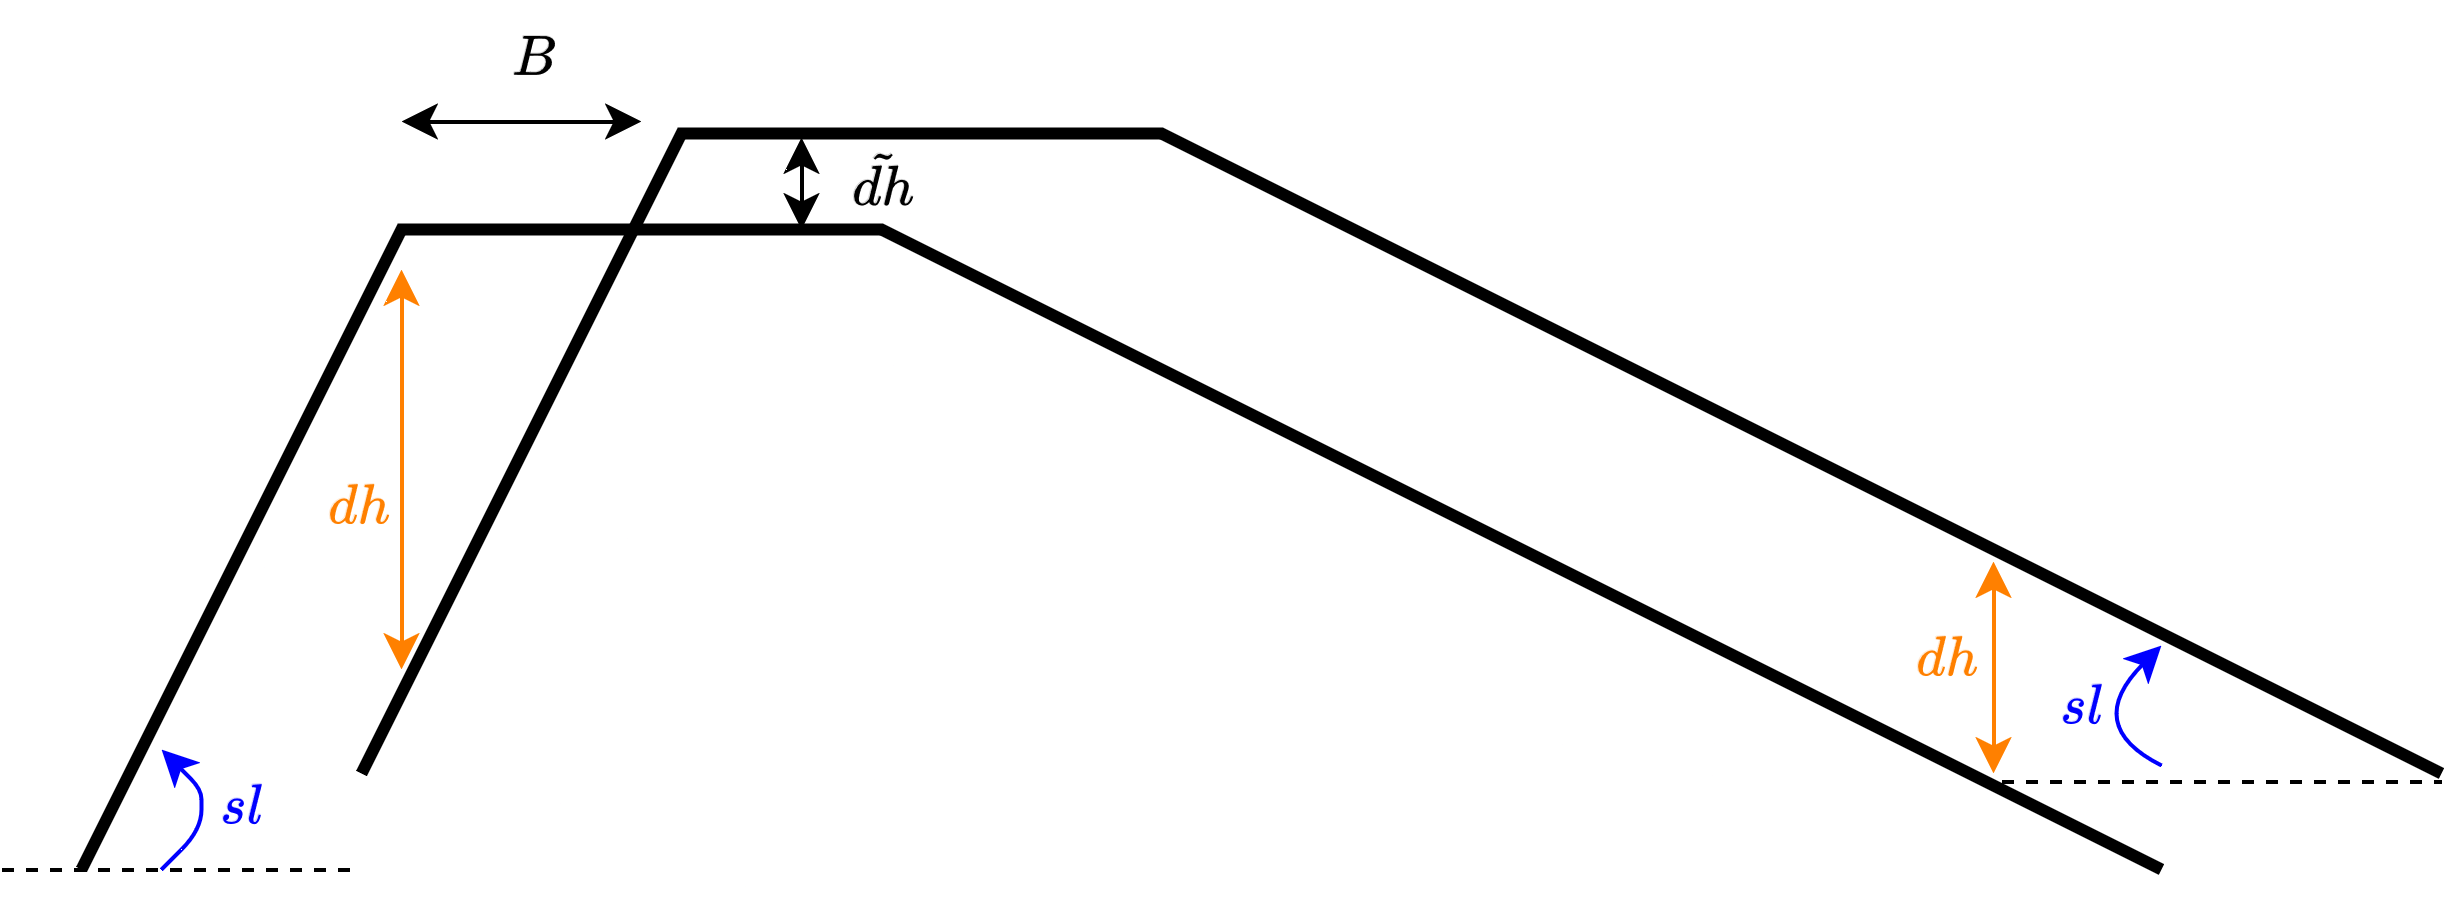
\includegraphics[width=\linewidth]{Images/Chap_6/Coregistration.png}
    \caption{Planimetric shift of magnitude $B$ and altimetric shift $\tilde{dh}$ between two \acrshort{dsm}s. We can see that local variations $\tilde{dh}$ vary depending on the slope $\sigma$. This diagram is in 2D, the angle of the planimetric shift and the azimut of the slope are therefore not represented.}
    \label{fig:coregistration}
\end{figure}

The three unknowns are $B$, $\beta$ and $\tilde{dh}$, as the slope parameters can be computed by any \acrshort{gis} software from the \acrshort{dsm}s. For instance, the slope of $\DSM_{true}$ is computed as:
\begin{align}\label{eq:slope}
    \sigma(x,y) = \dfrac{1}{8}\sqrt{\left(\dfrac{\DSM_{true}\ast k_x(x,y)}{r_x}\right)^2 + \left(\dfrac{\DSM_{true}\ast k_y(x,y)}{r_y}\right)^2}
\end{align}
where $\ast$ denotes a convolution with two kernels $k_x=\begin{bmatrix}
-1 & 0 & 1\\
-2 & 0 & 2 \\
-1 & 0 & 1
\end{bmatrix}$, $k_y=\begin{bmatrix}
-1 & -2 & -1\\
0 & 0 & 0 \\
1 & 2 & 1
\end{bmatrix}$, and $r_x$, $r_y$ are the resolution in $x$ and $y$. We will use the slope in the evaluation of the different metrics.

The unknowns $B$, $\beta$ and $\tilde{dh}$ are determined by a least square optimization problem. Because the \acrshort{dsm} is not expressed analytically, the optimisation is not guaranteed to be exact. Multiple iterations of the planimetric and altimetric shift estimation lead to a better final result. An illustration of the co-registration process is presented in \Cref{fig:coregistration_image}.

The problem we encounter is that the \acrshort{dsm} obtained from photogrammetry already possess some errors. In the least squared minimization problem, the residuals computed from the difference between the ground truth \acrshort{dsm} and the photogrammetry \acrshort{dsm} therefore also contain those errors. This deteriorates the quality of the co-registration. However, it remains the best solution for co-registering \acrshort{dsm}s. We apply this co-registration to our data, before computing any metric. The different metrics we consider will be presented in the following section. 

\begin{figure}
    \centering
    \begin{subfigure}[t]{0.48\linewidth}
        \centering
        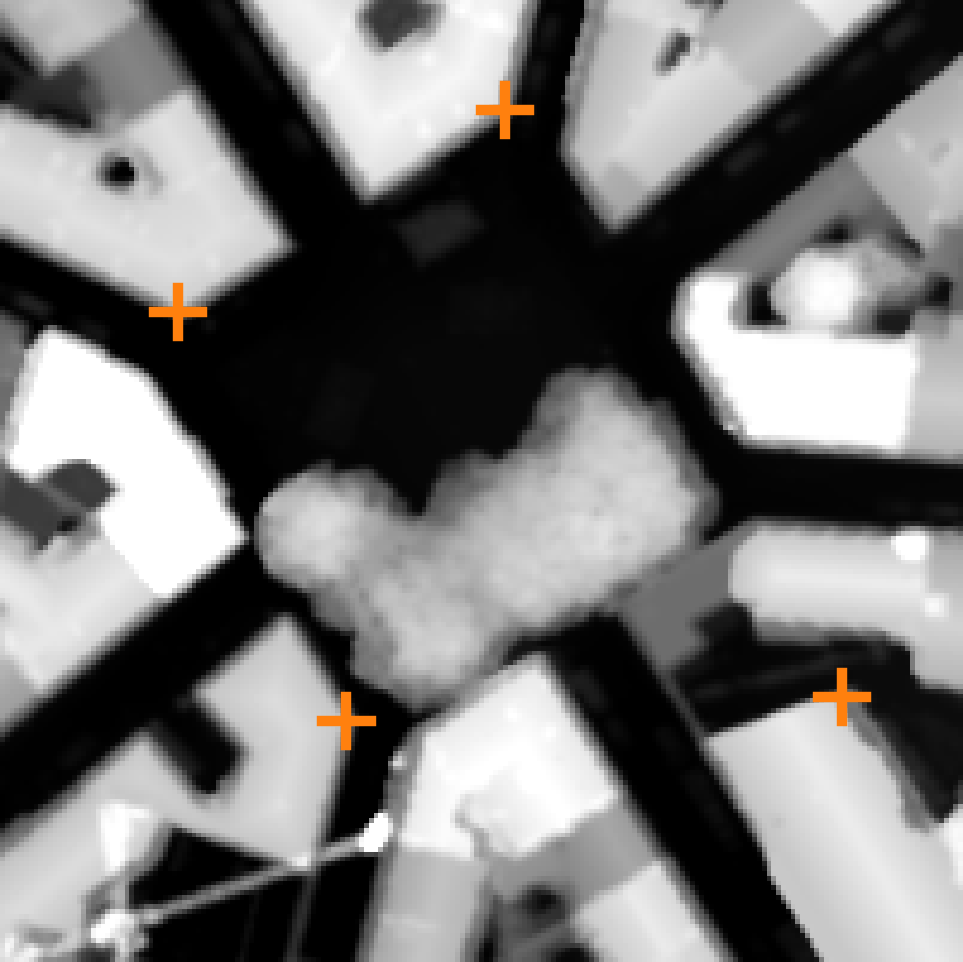
\includegraphics[width=\linewidth]{Images/Chap_6/coregisration_planimetric_shift_gt_toulouse.png}
        \caption{Ground Truth \acrshort{dsm}}
        \label{fig:coregistration_planimetric_gt}
    \end{subfigure}\hfill
    \begin{subfigure}[t]{0.48\linewidth}
        \flushright
        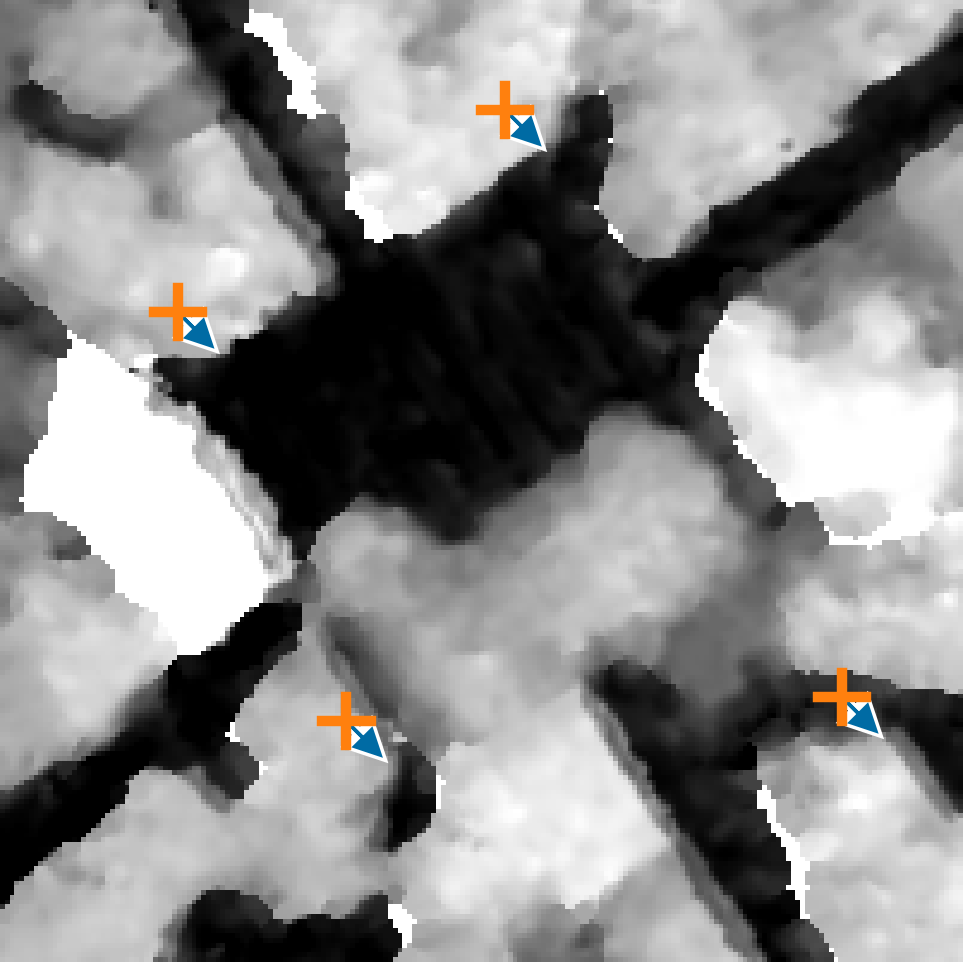
\includegraphics[width=\linewidth]{Images/Chap_6/coregisration_planimetric_shift_cars_toulouse.png}
        \caption{CARS \acrshort{dsm}}
        \label{fig:coregistration_planimetric_cars}
    \end{subfigure}\\
    \begin{subfigure}[t]{\linewidth}
        \centering
        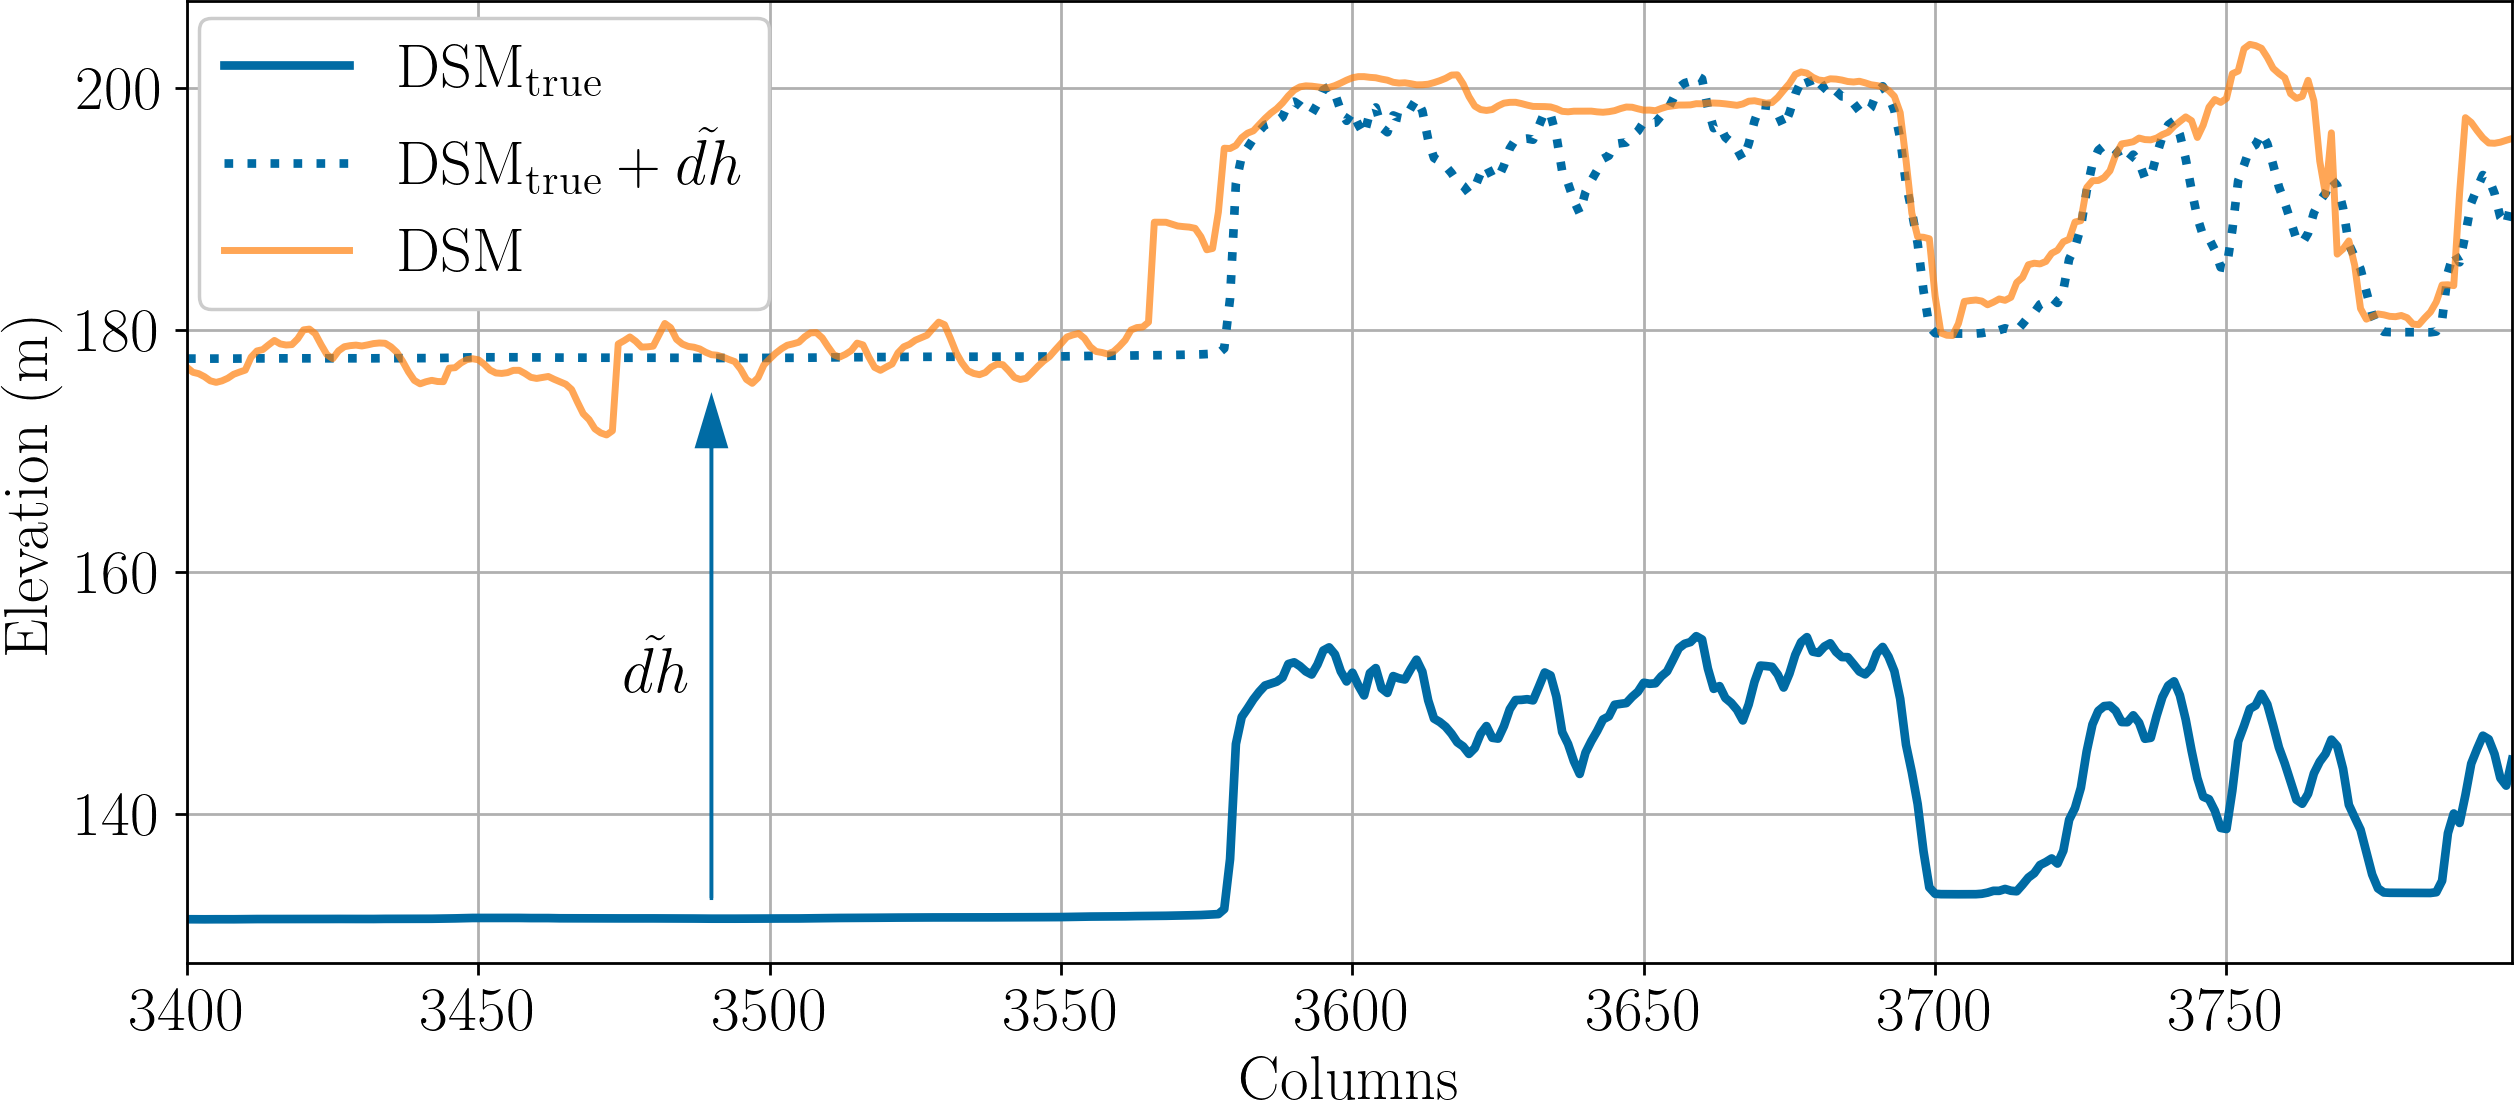
\includegraphics[width=\linewidth]{Images/Chap_6/coregisration_altimetric_shift_toulouse.png}
        \caption{Elevation along a row of the \acrshort{dsm}}
        \label{fig:coregistration_altimetric}
    \end{subfigure}
    \caption{Planimetric shift and altimetric shift from the co-registration step over the city of Toulouse. In \Cref{fig:coregistration_planimetric_gt,fig:coregistration_planimetric_cars}, reference points in orange are located at the same row and columns in the two \acrshort{dsm}s. The planimetric shift is indicated with blue arrows. \Cref{fig:coregistration_altimetric} presents the altimetric shift between the two \acrshort{dsm}s.}
    \label{fig:coregistration_image}
\end{figure}

\subsection{Configuration of the Photogrammetry Pipeline}
This sections provides technical information about the configuration of the CARS pipeline used to process the satellite images.

We used the Copernicus DEM with a 30m resolution as the reference altitude, as the SRTM elevation models were not available for high latitudes, in Norway for instance. We used the same range of considered disparity for every image: [-50pix, 50pix]. This range is quite high, especially for acquisition with a high altitude ratio $r_{alt}$, but insures we are not limited to a restrictive range of possible elevations.

Although we developed a method for creating disparity intervals which works for both the CENSUS and MC-CNN cost functions, we will only present results using the CENSUS cost function. Two reasons motivate this choice. First, due to the quantity of scenes and the variety of analysis completed, it would quickly become quite overwhelming to present each result for both cost functions, especially when there is no major difference between the two. Secondly, we observed in the previous chapter that disparity intervals obtained using CENSUS were less accurate than those using MC-CNN. As we favor accuracy above interval size, we chose to use the CENSUS cost function throughout our results, as validating the accuracy requirements for CENSUS insures that they are also validated using MC-CNN. We verified that they were no unexpected behaviour for MC-CNN intervals across scenes, and as nothing worth noticing appeared, we did not dive into so many details as we did for the CENSUS intervals.  

The following paragraph is a detailed list of the parameters used in the pipeline. The CENSUS cost function was computed using a 5$\times$5 window. The SGM penalties used for regularizing the CENSUS cost volume were $P_1=8$ and $P_2=32$. Disparity intervals were produced using a possibility threshold of $0.9$. Intervals were regularized in low confidence areas for which the confidence from ambiguity was bellow $0.6$. For each regularized pixel, we took the $0.9$\ith upper and $10$\ith lower quantiles over a low confidence area that extended 3 rows above and below. A V-fit refinement step was used to get sub-pixel disparities. Pixels that did not validate the cross-checking criterion from \cref{eq:cross-checking} were not considered for triangulation. Triangulated 3D points were filtered using \cref{eq:statistical_outlier} with $k=5$ and $N=50$, and \cref{eq:small_components} with $D_{max}=3$m and $N_{min}=50$. The rasterization from \cref{eq:rasterization} used $\sigma=0.3$m and $r=3$m.

\section{Metrics for Evaluating Elevation Intervals}\label{sec:metrics_elevation}
\todoroman{Je vais lire les commentaires de la section sur les métriques des intervalles de disparité et les appliquer ici aussi.}\commanue{A voir si tu peux pas mettre un schéma comme Gabriela dans sa présentation pour illustrer}
We introduce here the metrics used to evaluate the performances of elevation intervals. The metrics are not exactly the same as in \Cref{sec:metrics_disparity}, as we now reason with elevations instead of disparities. In order to stay consistent, we consider the metrics introduced for disparity intervals and adapt them to elevation intervals\commanue{les deux phrases précédentes sont un peu redondantes entre elles, je garderais que la deuxième}. 

We will refer to the true elevation as $\DSM_{true}$, the predicted elevation as $\DSM$ and the elevation intervals as $[\underline{\DSM},~\overline{\DSM}]$.

Similarly\commanue{Donc même remarque que pour les disparités, je mettrais des sous-sous-sections pour que l'on voit bien apparaître les différentes métrqiues} to \Cref{sec:metrics_disparity}, the first metric is the proportion of correct intervals, \ie the proportion of intervals containing the ground truth. We call this metric the accuracy $Z_{acc}$:
\begin{align}\label{eq:relative_accuracy_elevation}
    Z_{acc} = \dfrac{\#\{\DSM_{true} ~|~ \st ~\DSM_{true}\in [\underline{\DSM},~\overline{\DSM}]\}}{\#\{\DSM_{true}\}}
\end{align}
We want to maximize the accuracy. We also keep the objective of $90\%$ accuracy for our method, which was verified for the disparity intervals.

We are also interested in the evaluating\comloic{"evaluation" ou alors sans le "the", je te laisse voir} the magnitude of the error\comloic{singulier?}. We thus define the residual elevation error $Z_{\varepsilon}$ for all intervals that do not contain the ground truth as:
\begin{align}
    Z_\varepsilon=\dfrac{1}{r_{alt}} \cdot\median \left( \min(|\DSM_{true}-\overline{DSM}, ~ |\DSM_{true}-\underline{DSM}|)\right)\label{eq:residual_error_elevation}
\end{align}
where $r_{alt}$ is the disparity to altitude ratio (or altimetric ratio), \ie the elevation difference resulting from a shift of one disparity. We want $Z_\varepsilon$ error to be as close to 0 as possible. $r_{alt}$ has been computed alongside the epipolar grids (\Cref{sec:epipolar_geometry}). Dividing by the ratio $r_{alt}$ effectively converts $\min(|\DSM_{true}-\overline{DSM}|, |\DSM_{true}-\underline{DSM}|)$ from meters to pixels. If we do not make this conversion, an error of one disparity pixel in the dense matching step might result in an elevation error of 1m in a scene, and 2m in another\comloic{elle est bizarre cette phrase non ? Avec cette conversion, une erreur de 1pixel en disp peut toujours représenter 1m ou 2m sur le DSM en fonction de la config géo non? C'est juste que grace à la conversion tu vas toujours comparer des pixels pour t'affranchir de ce soucis. Mais tu supprimes pas le fait que 1pixel peut correspondre à 1m ou 2m.}. With this conversion, we can compare $Z_\varepsilon$ for stereo pairs with different convergence angles. For our data\commanue{As regards the data we consider?}, \Cref{tab:angle_coupling_pleiades} indicates that the convergence angles vary between $5\degree$ and $30\degree$. 

Those two previous metrics allow to measure the accuracy and errors of elevation intervals. To evaluate the size of intervals, we use the relative elevation size $Z_{size}$ defined as :
\begin{align}\label{eq:relative_size_elevation}
    Z_{size} = \dfrac{1}{r_{alt}}\median(\overline{DSM}-\underline{DSM})
\end{align}
We divide by the altimetric ratio for the same reasons as in $Z_\varepsilon$, \ie to compare stereo pairs with different convergence angles. We want the relative elevation size to be as close to zero as possible. $Z_{size}$ is similar to $s_{rel}$ defined in \cref{eq:relative_size_disparity} from \Cref{sec:metrics_disparity}.

\begin{comment}
    The final metric to evaluate the size of the intervals is the relative elevation overestimation $Z_{o}$, defined as:
    \begin{align}\label{eq:relative_overestimation_elevation}
        Z_{o} = 1-\median(\dfrac{\max(|\DSM_{true}-\DSM|,~\cdot r_{alt})}{\overline{DSM}-\underline{DSM}})
    \end{align}
    \todoroman{La definir en deux fois. Une fois comme orel avec un schéma, et ensuite on ajoute le ralt}
    This metric is similar to the relative overestimation $o_{rel}$ from \cref{eq:relative_overestimation_disparity}, as it aims to measure the proportion of the size of intervals that is superfluous. We use this metric because we accept to have very large intervals if the error $|\DSM_{true}-\DSM|$ is also very large, \ie if $Z_{o}$ is low. The main difference with $o_{rel}$ is that we do not simply consider the \acrshort{dsm} error $|\DSM_{true}-\DSM|$, as it can get very low, or can even be null. When $|\DSM_{true}-\DSM|$ reaches values close to 0, $ Z_{o}$ could reach high values near 1 (\ie, $100\%$ of the interval is superfluous) even if the interval size is not that large. For instance, if $|\DSM_{true}-\DSM|$ is about 1cm, and the interval is just 1m large, then $99\%$ of the size of the interval would be considered superfluous, although 1m is usually considered to be a small interval. To avoid those extreme values, we consider the maximum $\max(|\DSM_{true}-\DSM|, \cdot r_{alt})$ in the expression of $Z_{o}$, so that if $|\DSM_{true}-\DSM|$ gets too low, then we replace it by $\cdot r_{alt}$. Otherwise we keep $|\DSM_{true}-\DSM|$.
\end{comment}


\begin{remark}
    \begin{comment}
        We did not have the problem of $|d_{true}- \tilde{d}|$ being too small in $o_{rel}$ as we instead used the maximal error over a low confidence area (\ie the area considered for the regularization). 
    \end{comment}
    In the rasterization process, 3D points from low confidence area are mixed with points from high confidence areas. We therefore cannot define regularization areas\commanue{en lisant ça fait bizarre le terme de regularisation. Pour éviter s'embrouiller avec SGM ou d'autres filtrage, je mettrais bien interval regularization, histoire d'éviter toute ambiguïté ;)} in the final \acrshort{dsm}. The relative over-estimation $o_{rel}$ has therefore no equivalent for elevation intervals.  
\end{remark}

\section{Elevation Intervals Results}\label{sec:results_elevation}
\begin{table}[ht]
    \centering
    \begin{tabular}{|c||c|c|c|c|c|c|}
        \hline
        Scene & $Z_{acc}$ & $Z_\varepsilon$ (pix) & $Z_{size}$ (pix) & $r_{alt}$ (m/pix) & invalid
        \\\hline\hline
        Bordeaux & 89.3$\%$ & 0.56 & 4.18 & 1.24  & 21.5$\%$\\\hline
        Graasubreen & 99.7$\%$ & 0.12 & 1.96 & 1.32  & 27.5$\%$\\\hline
        Hellmem & 98.8$\%$ & 2.76 & 2.02 & 1.32  & 34.7$\%$\\\hline
        Grenoble & 93.1$\%$ & 0.87 & 3.99 & 1.06  & 6.4$\%$\\\hline
        Langfjordjøkelen & 99.4$\%$ & 0.30 & 2.16 & 1.35  & 13.9$\%$\\\hline
        Monaco & 90.3$\%$ & 0.57 & 3.76 & 0.99  & 41.9$\%$\\\hline
        Montpellier & 89.1$\%$ & 0.28 & 2.05 & 3.64  & 1.9$\%$\\\hline
        Paris & 84.6$\%$ & 0.46 & 2.01 & 5.78  & 3.0$\%$\\\hline
        Peyto & 98.9$\%$ & 0.18 & 2.08 & 1.66  & 18.3$\%$\\\hline
        Pic du midi & 98.1$\%$ & 0.20 & 2.41 & 1.01  & 7.5$\%$\\\hline
        Toulouse & 92.0$\%$ & 0.38 & 2.04 & 2.43  & 6.9$\%$\\\hline
    \end{tabular}
    \caption{Elevation metrics for the different stereo pairs. The last column indicates the proportion of invalid pixels in the considered \acrshort{dsm}s.}
    \label{tab:elevation_metrics_global}
\end{table}

\begin{figure}
    \begin{subfigure}[t]{0.553\linewidth}
        \flushleft
        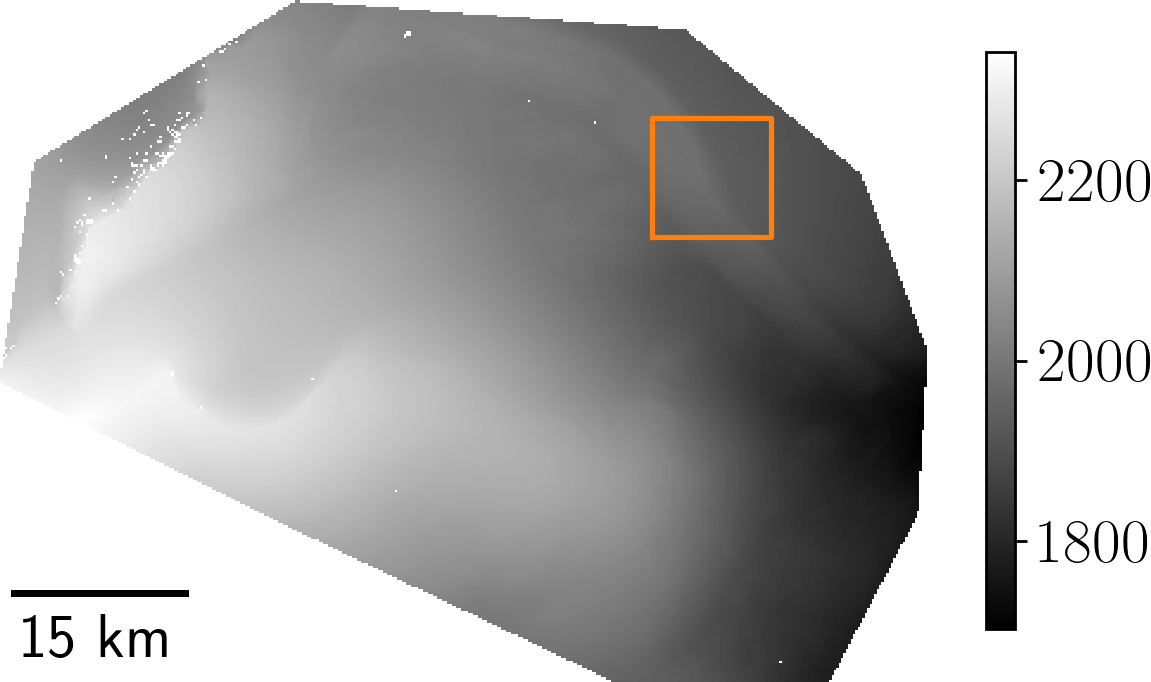
\includegraphics[width=\linewidth]{Images/Chap_6/Graasubreen_dsm.png}
        \caption{Photogrammetry \acrshort{dsm}. Orange area is detailed in \Cref{fig:Graasubreen_zoom}}
        \label{fig:Graasubreen_dsm}
    \end{subfigure}
    \begin{subfigure}[t]{0.447\linewidth}
        \flushright
        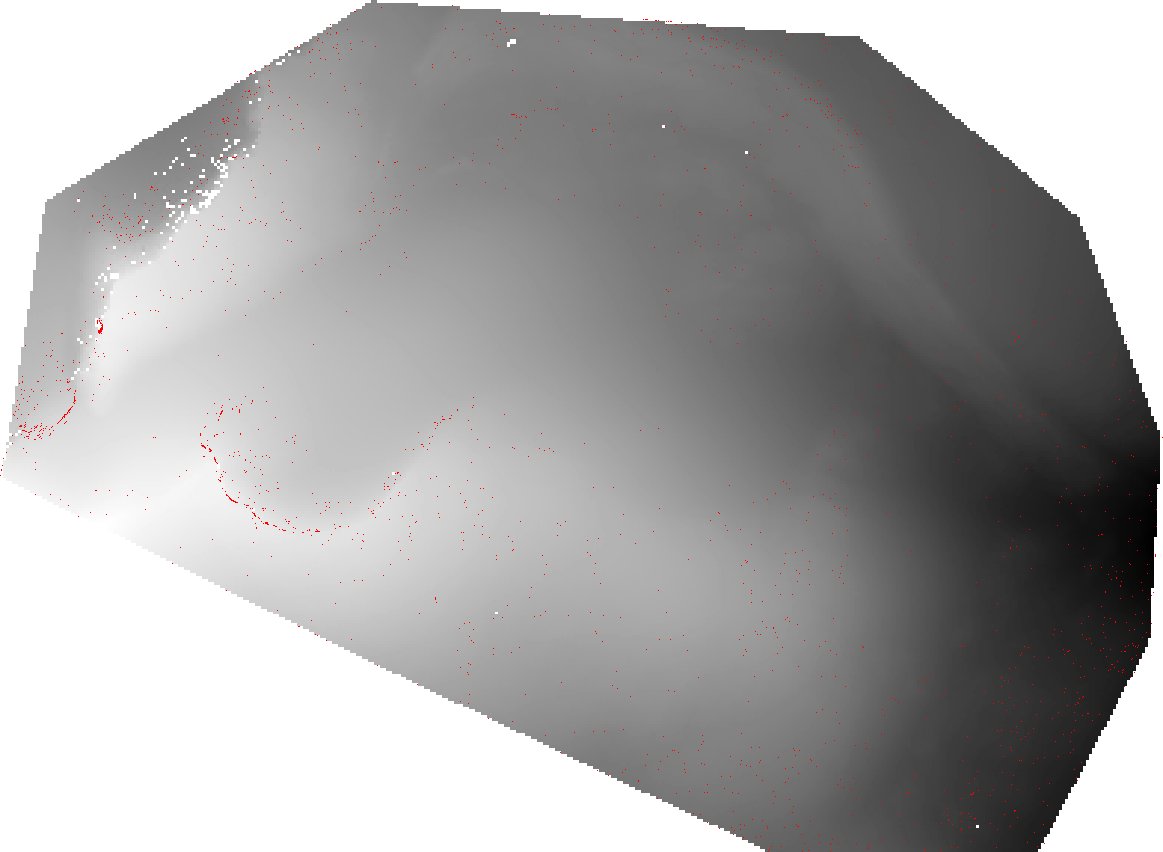
\includegraphics[width=\linewidth]{Images/Chap_6/Graasubreen_error.png}
        \caption{\acrshort{dsm} with wrong intervals in red.}
        \label{fig:Graasubreen_error}
    \end{subfigure}
    \caption{\acrshort{dsm} without and with wrong intervals over Graasubreen scene}
    \label{fig:Graasubreen_global}
\end{figure}

\begin{figure}
    \begin{subfigure}[t]{0.49\linewidth}
        \flushleft
        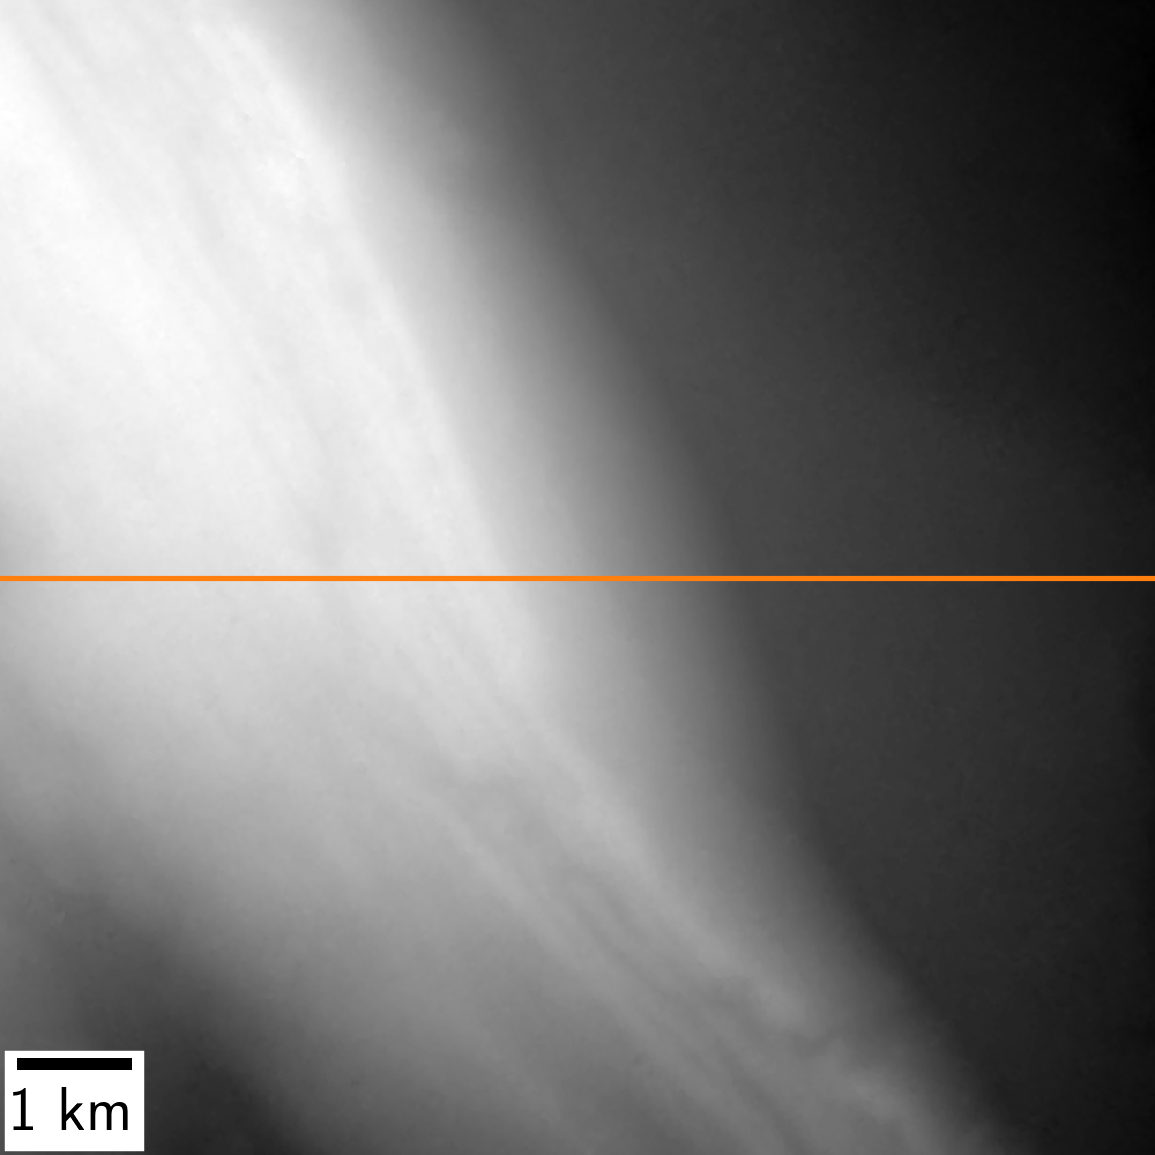
\includegraphics[width=\linewidth]{Images/Chap_6/Graasubreen_dsm_zoom.png}
        \caption{Photogrammetry \acrshort{dsm}. Orange line is detailed in \Cref{fig:Graasubreen_zoom_row}}
        \label{fig:Graasubreen_dsm_zoom}
    \end{subfigure}\hfill
    \begin{subfigure}[t]{0.49\linewidth}
        \flushright
        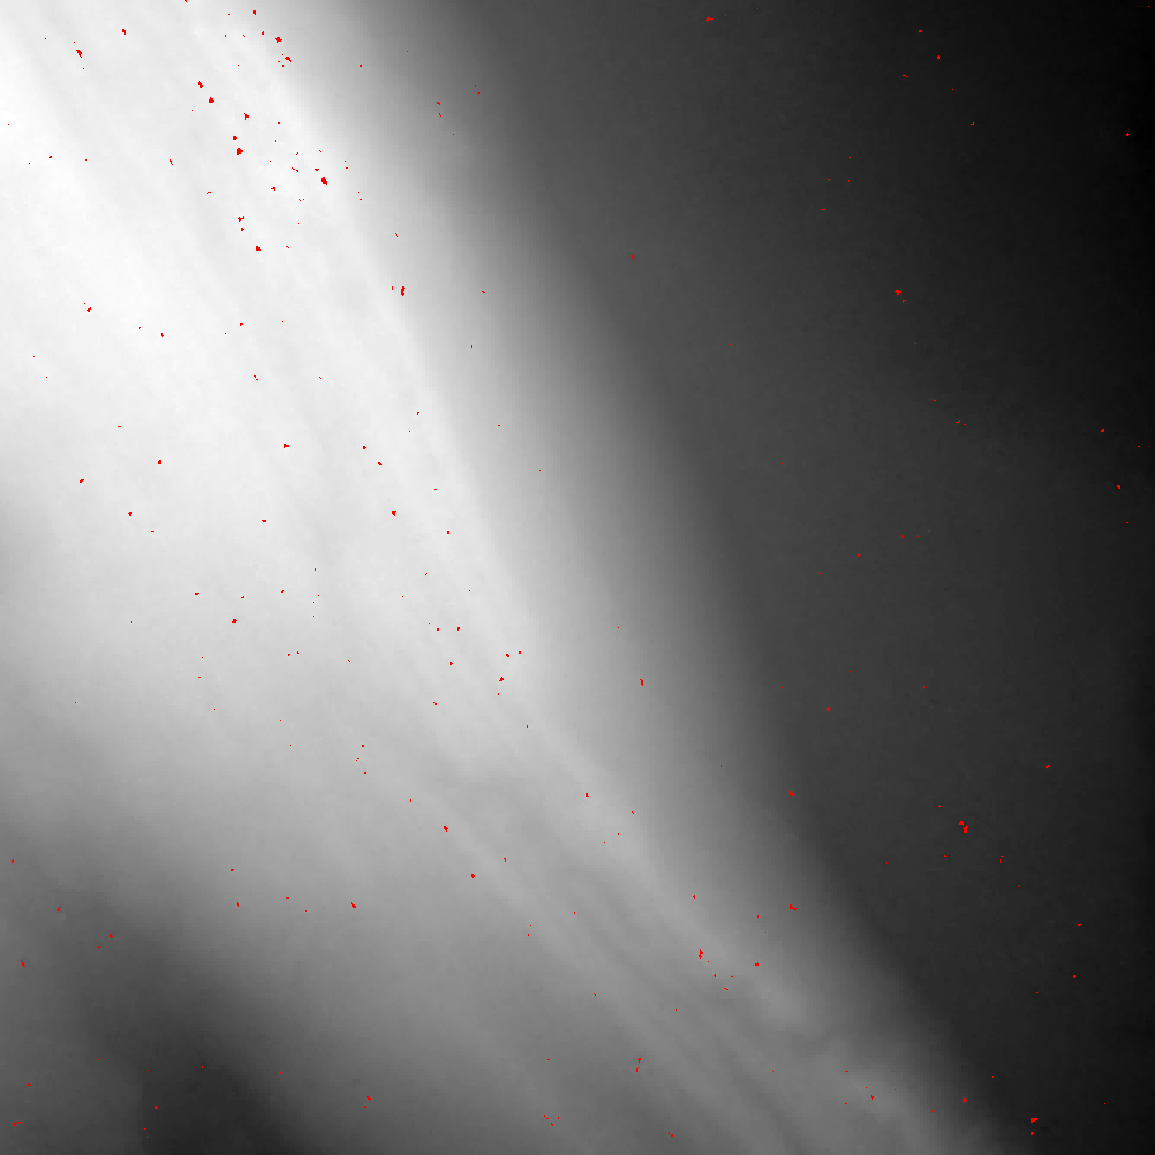
\includegraphics[width=\linewidth]{Images/Chap_6/Graasubreen_error_zoom.png}
        \caption{\acrshort{dsm} with wrong intervals in red.}
        \label{fig:Graasubreen_error_zoom}
    \end{subfigure}
    \begin{subfigure}[t]{\linewidth}
        \centering
        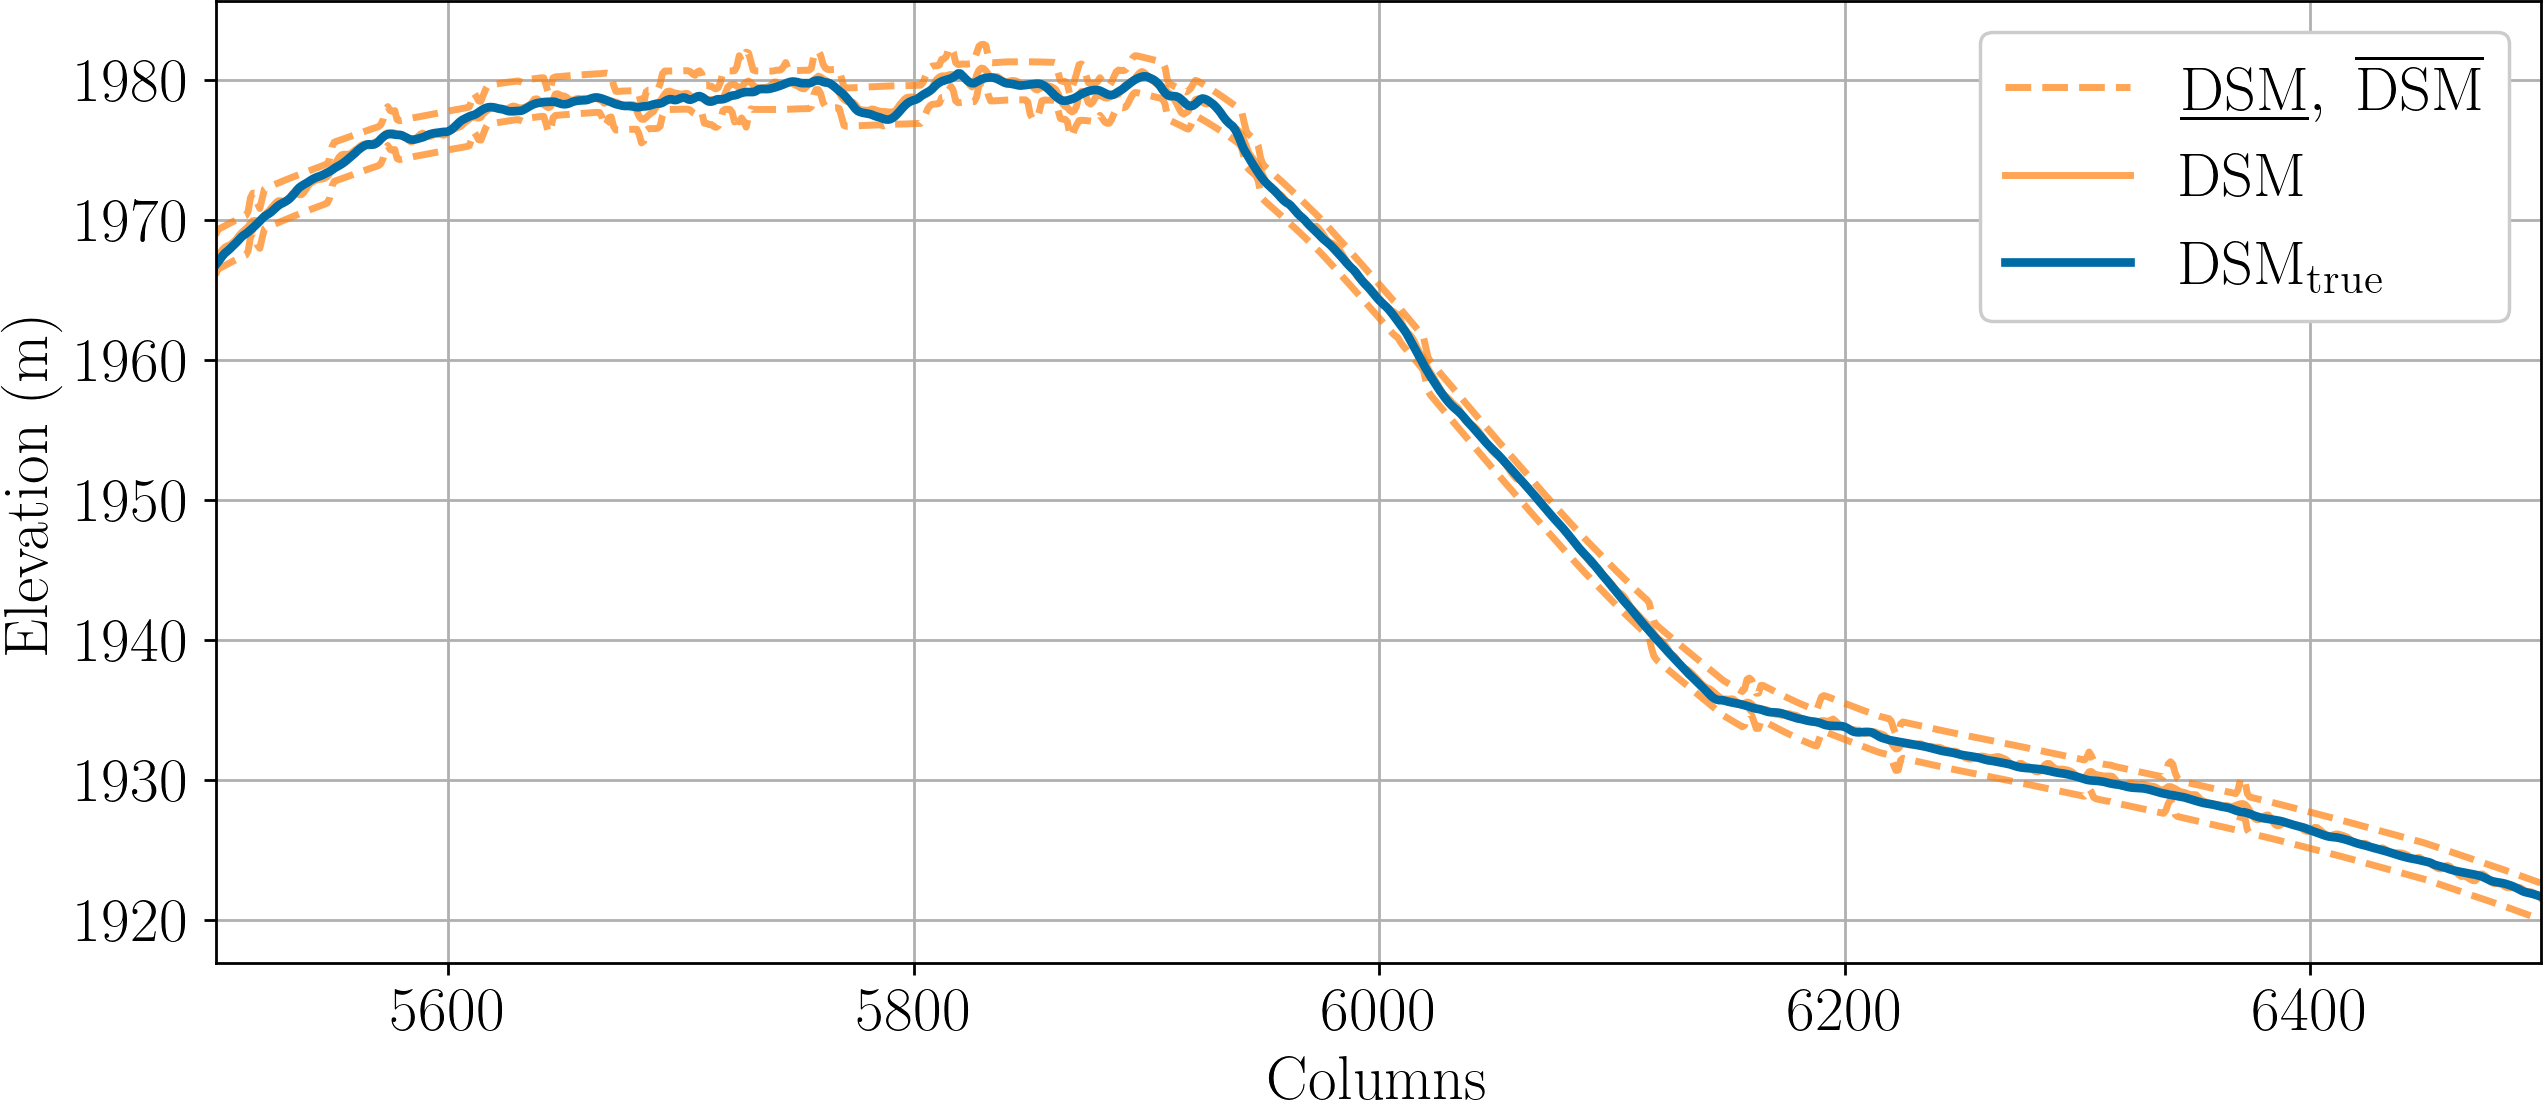
\includegraphics[width=\linewidth]{Images/Chap_6/Graasubreen_row_1500.png}
        \caption{\acrshort{dsm}, ground truth and elevation intervals along the orange line of \Cref{fig:Graasubreen_dsm_zoom}}
        \label{fig:Graasubreen_zoom_row}
    \end{subfigure}
    \caption{Details of the Graasubreen \acrshort{dsm}. This area corresponds to the orange square from \Cref{fig:Graasubreen_dsm}.}
    \label{fig:Graasubreen_zoom}
\end{figure}


\begin{figure}
    \begin{subfigure}[t]{0.549\linewidth}
        \flushleft
        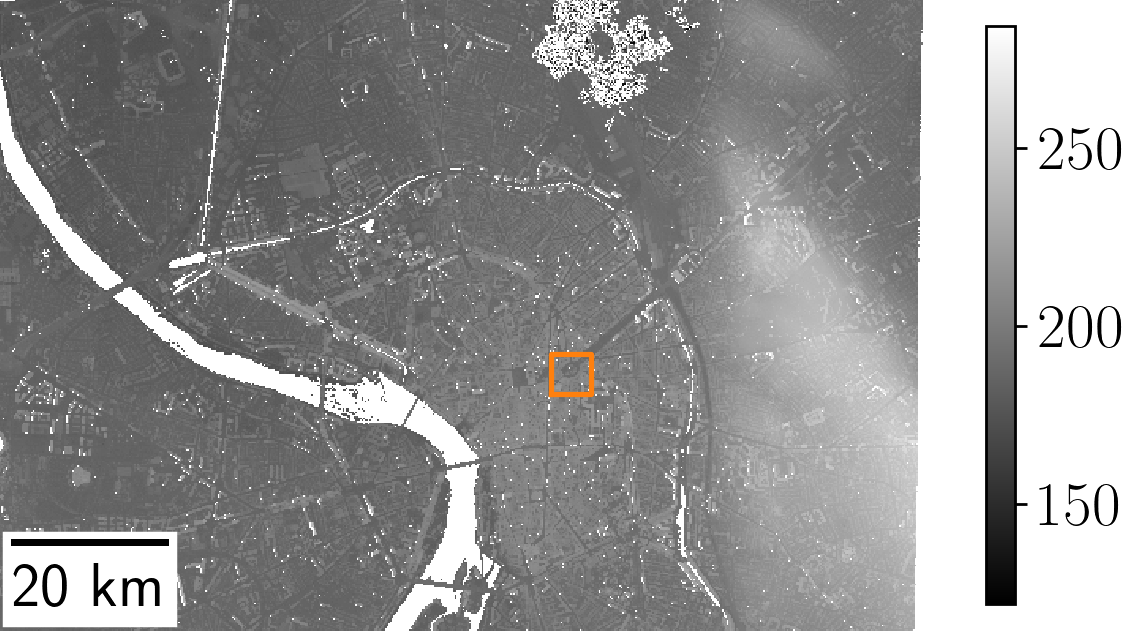
\includegraphics[width=\linewidth]{Images/Chap_6/Toulouse_dsm.png}
        \caption{Photogrammetry \acrshort{dsm}. Orange area is detailed in \Cref{fig:toulouse_zoom}}
        \label{fig:toulouse_dsm}
    \end{subfigure}
    \begin{subfigure}[t]{0.451\linewidth}
        \flushright
        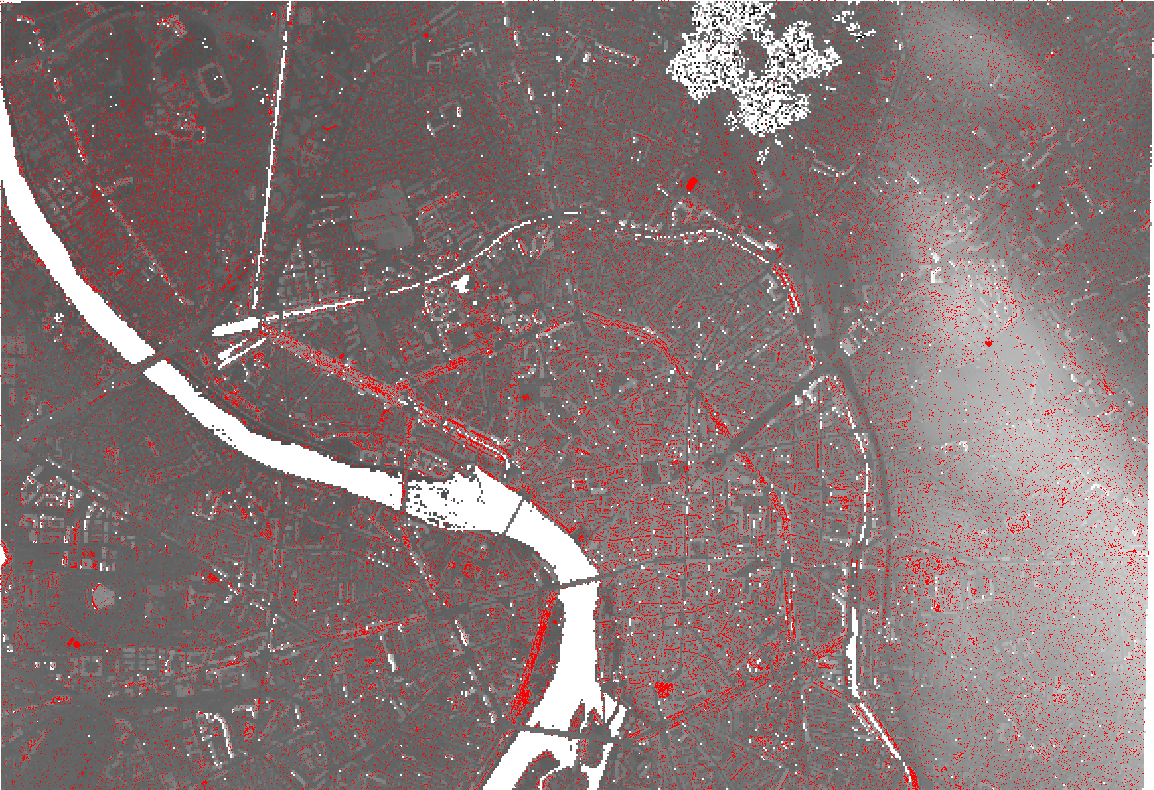
\includegraphics[width=\linewidth]{Images/Chap_6/Toulouse_error.png}
        \caption{\acrshort{dsm} with wrong intervals in red.}
        \label{fig:toulouse_error}
    \end{subfigure}
    \caption{\acrshort{dsm} without and with wrong intervals over Toulouse scene}
    \label{fig:toulouse_global}
\end{figure}



\begin{figure}
    \begin{subfigure}[t]{0.49\linewidth}
        \flushleft
        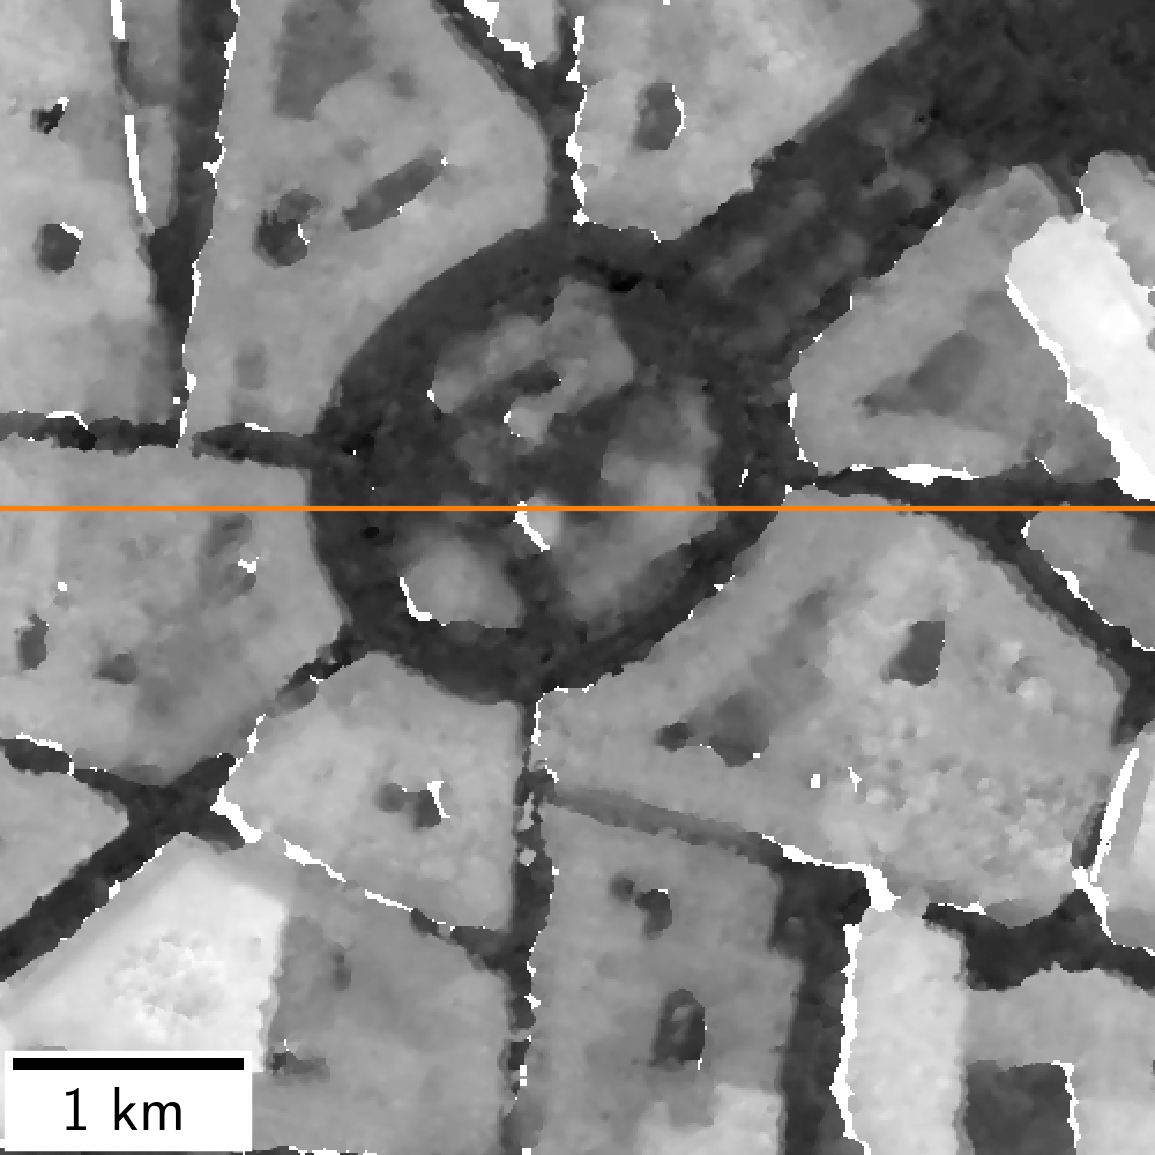
\includegraphics[width=\linewidth]{Images/Chap_6/Toulouse_dsm_zoom.png}
        \caption{Photogrammetry \acrshort{dsm}. Orange line is detailed in \Cref{fig:toulouse_zoom_row}}
        \label{fig:toulouse_dsm_zoom}
    \end{subfigure}\hfill
    \begin{subfigure}[t]{0.49\linewidth}
        \flushright
        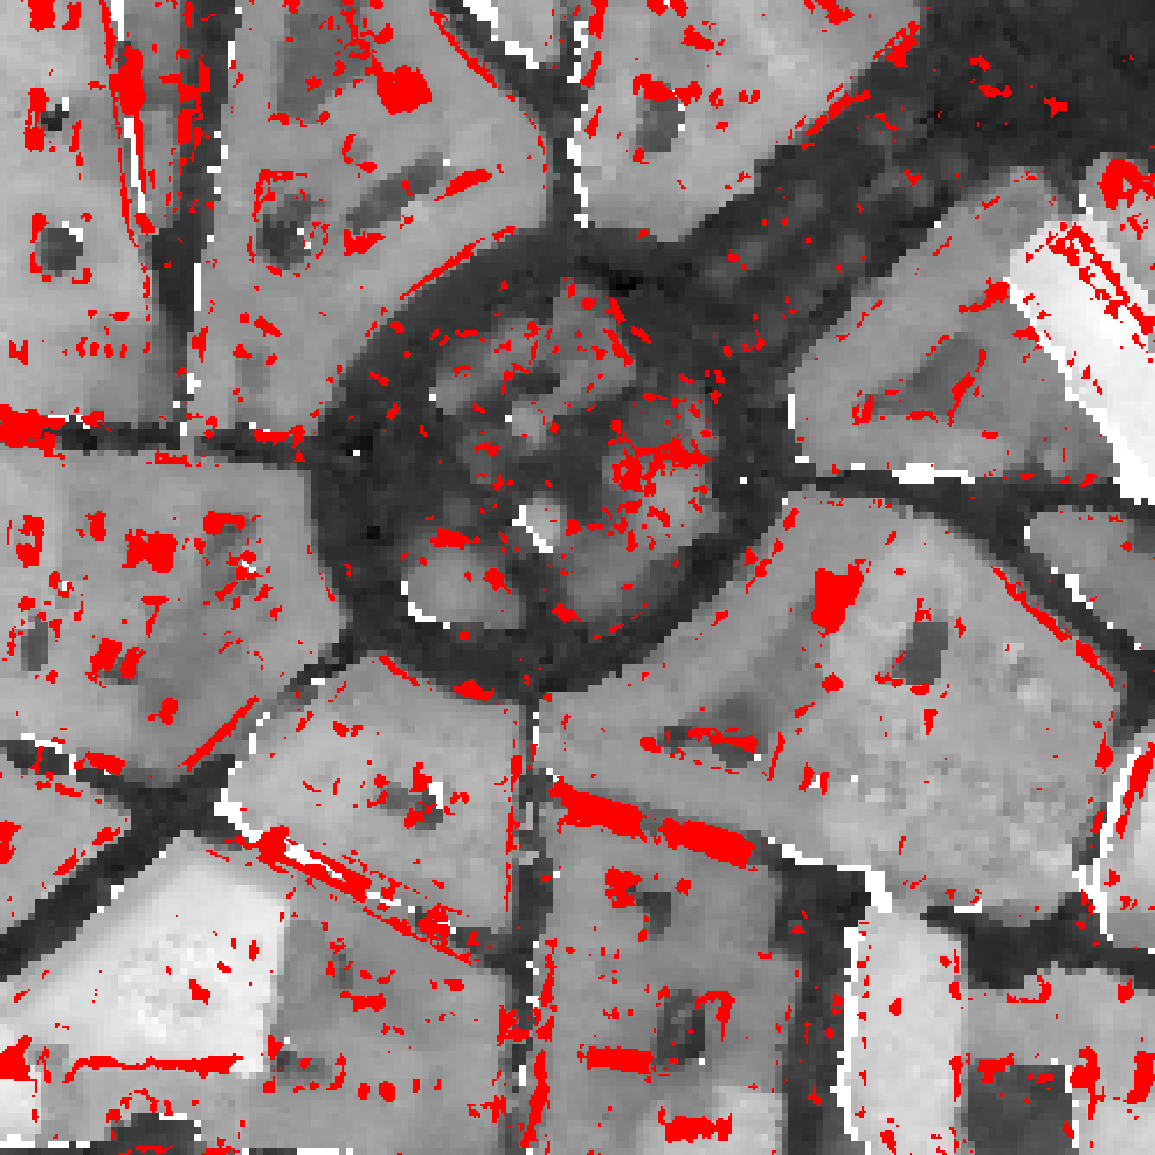
\includegraphics[width=\linewidth]{Images/Chap_6/Toulouse_error_zoom.png}
        \caption{\acrshort{dsm} with wrong intervals in red.}
        \label{fig:toulouse_error_zoom}
    \end{subfigure}
    \begin{subfigure}[t]{\linewidth}
        \centering
        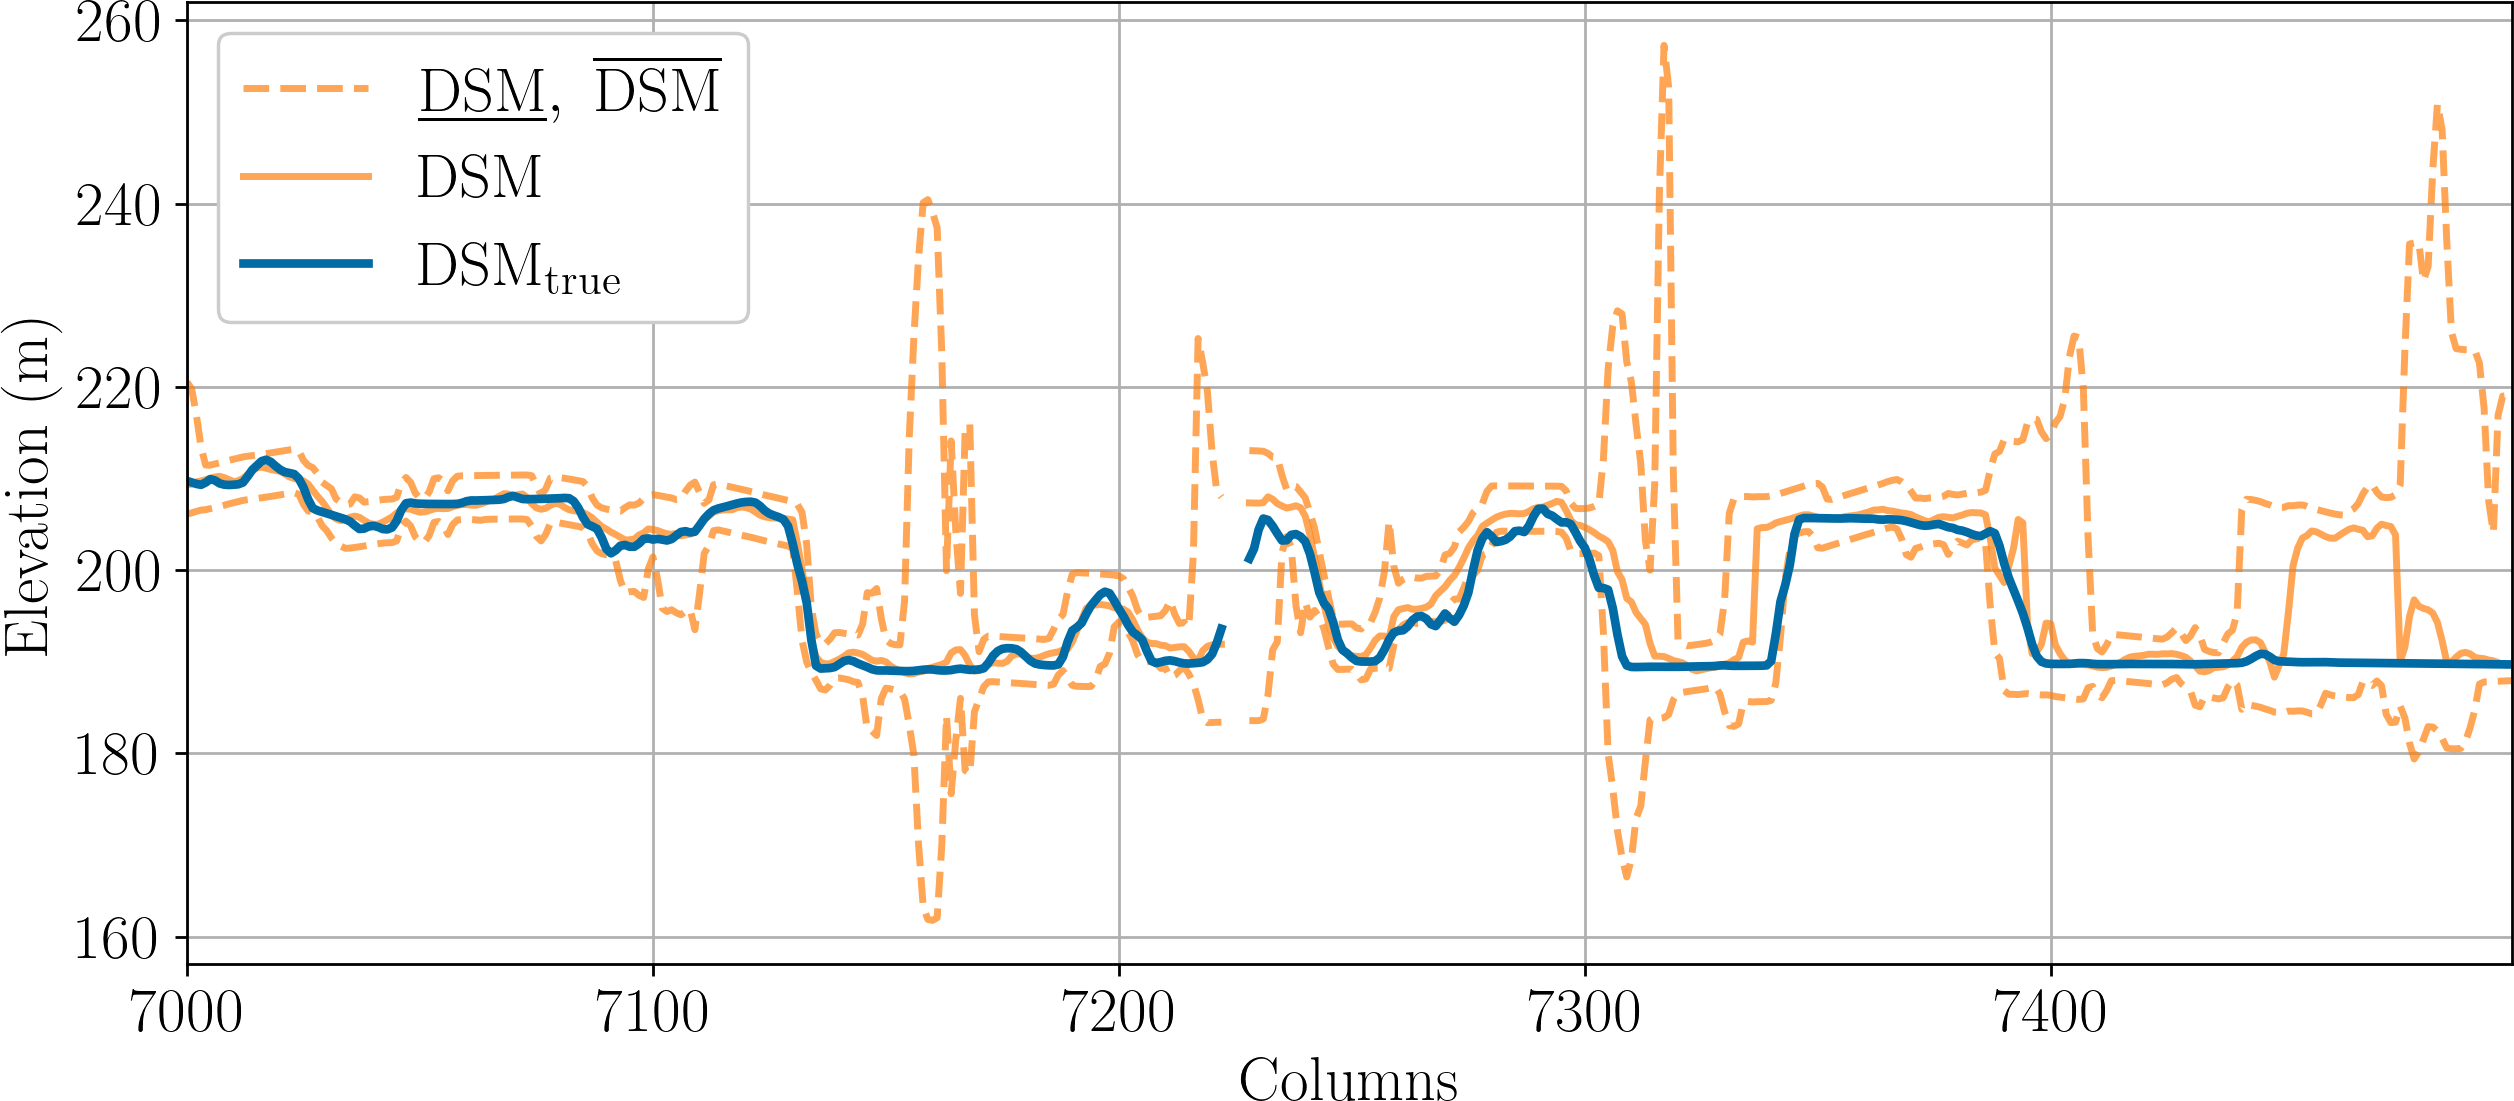
\includegraphics[width=\linewidth]{Images/Chap_6/Toulouse_row_4720.png}
        \caption{\acrshort{dsm}, ground truth and elevation intervals along the orange line of \Cref{fig:toulouse_dsm_zoom}}
        \label{fig:toulouse_zoom_row}
    \end{subfigure}
    \caption{Detailed \acrshort{dsm} over Wilson square, Toulouse. This area corresponds to the orange square from \Cref{fig:toulouse_dsm}.}
    \label{fig:toulouse_zoom}
\end{figure}


The different metrics have been evaluated between the photogrammetry \acrshort{dsm} and the ground truth \acrshort{dsm}\commanue{the associated ground truth ?}. Results are presented in \Cref{tab:elevation_metrics_global}. We also displayed for information the proportion of invalid pixels of each scene, in the last column of the table. A pixel is invalid if the ground truth \acrshort{dsm} or predicted \acrshort{dsm} do not contain any data for this pixel, or if it was masked by a water mask. Invalid pixels are therefore pixels which were not considered when computing the metrics.

\Cref{fig:Graasubreen_global,fig:Graasubreen_zoom,fig:toulouse_global,fig:toulouse_zoom} allow to qualitatively evaluate the performances of the elevation intervals. We can see that intervals seem to have better performances on rural scenes such as glaciers than on urban scenes. For instance, we can clearly see the wrong intervals of the Toulouse scene in \Cref{fig:toulouse_error}, while they are harder to distinguish for the Graasubreen scene in \Cref{fig:Graasubreen_error,fig:Graasubreen_error_zoom}. Another notable observation is that elevation intervals of the Graasubreen glacier in \Cref{fig:Graasubreen_zoom_row} are very small and do not vary in size, all along the considered cross section. This is not the case in the Toulouse scene (\Cref{fig:toulouse_zoom_row}), where intervals have varying sizes. They are relatively small from columns 7000 to 7100, but their size increases from column 7400 to 7500. We can see on the right of \Cref{fig:toulouse_zoom_row}, near column 7450, that their size allow to correctly contain the ground truth despite the difference between $\DSM$ and $\DSM_{true}$. However, there are some very large intervals, sometimes reaching $80$m of size, near columns 7150, or 7300. Those intervals can occur because the range of considered disparities in the dense matching step was $[-50, 50]$, for every scene. Converted into altitude, elevations intervals have a maximal size of $[-50\dot r_{alt}, 50\cdot r_{alt}]$, centered around the reference altitude (which can vary across the scene). This means that we can have maximal elevation intervals of size 243m in the case of Toulouse where $r_{alt}=2.43$. The previously observed intervals of size 80m in \Cref{fig:toulouse_zoom_row} thus originates from a disparity intervals of 33 pixels of size, \ie a third of the disparity intervals. We will see in section \ref{sec:unexplored_leads} that we could modify our method to filter the points leading to those intervals. For now, we will evaluate the method as it stands. 

\begin{remark}
    Following the previous discussion about the elevation intervals size, here are some reference interval size for information purposes. For the Monaco scene where $r_{alt}=0.99$, the largest interval has a size of $99$m and is centered around the reference altitude. For the Paris scene where  $r_{alt}=5.78$, the largest interval has a size of 578m.
\end{remark}

The following sections are dedicated to the discussion of each metric individually.

\subsection{Elevation accuracy}
The elevation accuracy $Z_{acc}$, defined in \cref{eq:relative_accuracy_elevation}, measures the proportions of intervals which contains the ground truth elevation, which we want to be as high as possible. The first observation is that the $90\%$ accuracy objective is validated on $8$ of the $11$ scenes we considered. In particular, the different glaciers as well as the Pic du Midi elevation intervals present a great accuracy between $98.1\%$ and $99.7\%$. The scenes that do not verify the objective are the urban stereo pairs over Bordeaux, Montpellier and Paris. In general, it seems that urban \acrshort{dsm}s have a lower accuracy than rural ones, which was to be expected as there are more steep variations of elevation in cities due to the presence of buildings. The Montpellier \acrshort{dsm} and Bordeaux \acrshort{dsm} are close to the $90\%$ objective, but intervals over Paris are accurate only $84.6\%$ of the time\commanue{alors là je trouve que la formulation fait très française "du temps" mais je ne sais pas si les anglais nous ont piqué la réplique}. We will see in \Cref{sec:other_errors} that some other sources of errors can explain why $Z_{acc}<90\%$ on those scenes, such as vibration of the satellite during images acquisition or ground truth non-synchronicity issues. Provided that those errors are not present, we can claim that elevation intervals are accurate enough. They correctly estimate the error committed during the dense matching step, and the propagation of disparity intervals to elevation intervals is properly carried out.

\subsection{Residual elevation error}
The residual elevation error $Z_\varepsilon$, defined in \cref{eq:residual_error_elevation}, estimates the gap between the intervals and the ground truth, when intervals do not contain the ground truth. We want it to be as small as possible. $Z_\varepsilon$ is less than, or almost equal to, half a pixel for the majority of scenes. This is really low. Because $Z_\varepsilon$ is the median of error, it means that half of wrong intervals are less that $Z_\varepsilon$ pixels away from one of the bounds of the elevation intervals. It means that extending the intervals by $Z_\varepsilon$ would divide by two the number of wrong intervals. For scenes validating the $90\%$ accuracy, $Z_\varepsilon$ provides an easy extension for obtaining intervals with $95\%$ accuracy. For instance on the Monaco scene, $Z_\varepsilon=0.57$pix, $r_{alt}=0.99$m/pix and $Z_{acc}=90.3\%$. Defining the extended intervals as:
\begin{align*}
    [\underline{\DSM}-Z_\varepsilon\cdot r_{alt}, \overline{\DSM}+Z_\varepsilon\cdot r_{alt}] \approx [\underline{\DSM}-0.56, \overline{\DSM}+0.56]
\end{align*}
As the accuracy is $90.3\%$, it means that $9.7\%$ of pixels are not accurate. Using $[\underline{\DSM}-0.56, \overline{\DSM}+0.56]$ would lead to a new accuracy of $90.3+\dfrac{9.7}{2}=95.15\%$\commanue{donc pour Monaco ça fait 95 mais par forcément pour toutes les scènes.}. 

There is one $Z_\varepsilon$ value that stands out, for the Hellmem scene where it equals $2.76$. We have to keep in mind that the accuracy for this scene is $98.8\%$, so that $Z_\varepsilon$ is only computed on $1.2\%$ of valid intervals, so that $Z_\varepsilon=2.76$ is therefore not necessarily a concerning observation as it concerns very few pixels. It is more surprising that it equals $0.12$ for the Graasubreen \acrshort{dsm} which already has the best accuracy $99.7\%$ out of all scenes. This translates the great performance of the elevation intervals estimation on this area.

\subsection{Relative elevation size}\commanue{là tu commentes les métriques globales. Si on prend un payasage naturel sur le paysage c'est quoi l'histogramme de la taille des intervalles, pareil sur un paysage urbain. Maintenant que j'ai compris le graphique tu peux reprendre les figures de Gabriela ;) Après ça peut être bien de visualiser la taille des intervalles qui varient sur un segment ou alors que faire une carte de la taille des intervalles en te limitant à une zone histoire que ça reste lisible}
The relative elevation size $Z_{size}$, defined in \cref{eq:relative_size_elevation}, estimates the size of intervals, both correct and incorrect. $Z_{size}$ is usually around 2 pixels wide. The Bordeaux, Grenoble and Monaco datasets are the only exceptions, were $Z_{size}$ is closer to 4 pixels in size. It does not seem to be correlated neither to the accuracy, nor to the altimetric ratio or acquisition angles of the satellites. In any case, 4 pixels is not ideal, but it is not excessively large either\commanue{Il faudrait le mettre en relation avec l'intervalle de disparité utilisé pour la recherche dans l'étape Pandora}. We can deduce from those values of $Z_{size}$ that the predicted \acrshort{dsm} is close to the true elevation. 

\Cref{fig:histogram_elevation_toulouse} presents the distributions of relative errors and relative sizes over the scene in Toulouse. It provides a more complete overview of the distribution of errors and sizes than simply the indicators $Z_\varepsilon$ and $Z_{size}$ which are defined as the median of those distributions. The distributions on other scenes have a similar shape. 
\begin{figure}
    \centering
    \begin{subfigure}[t]{0.5\linewidth}
        \flushright
        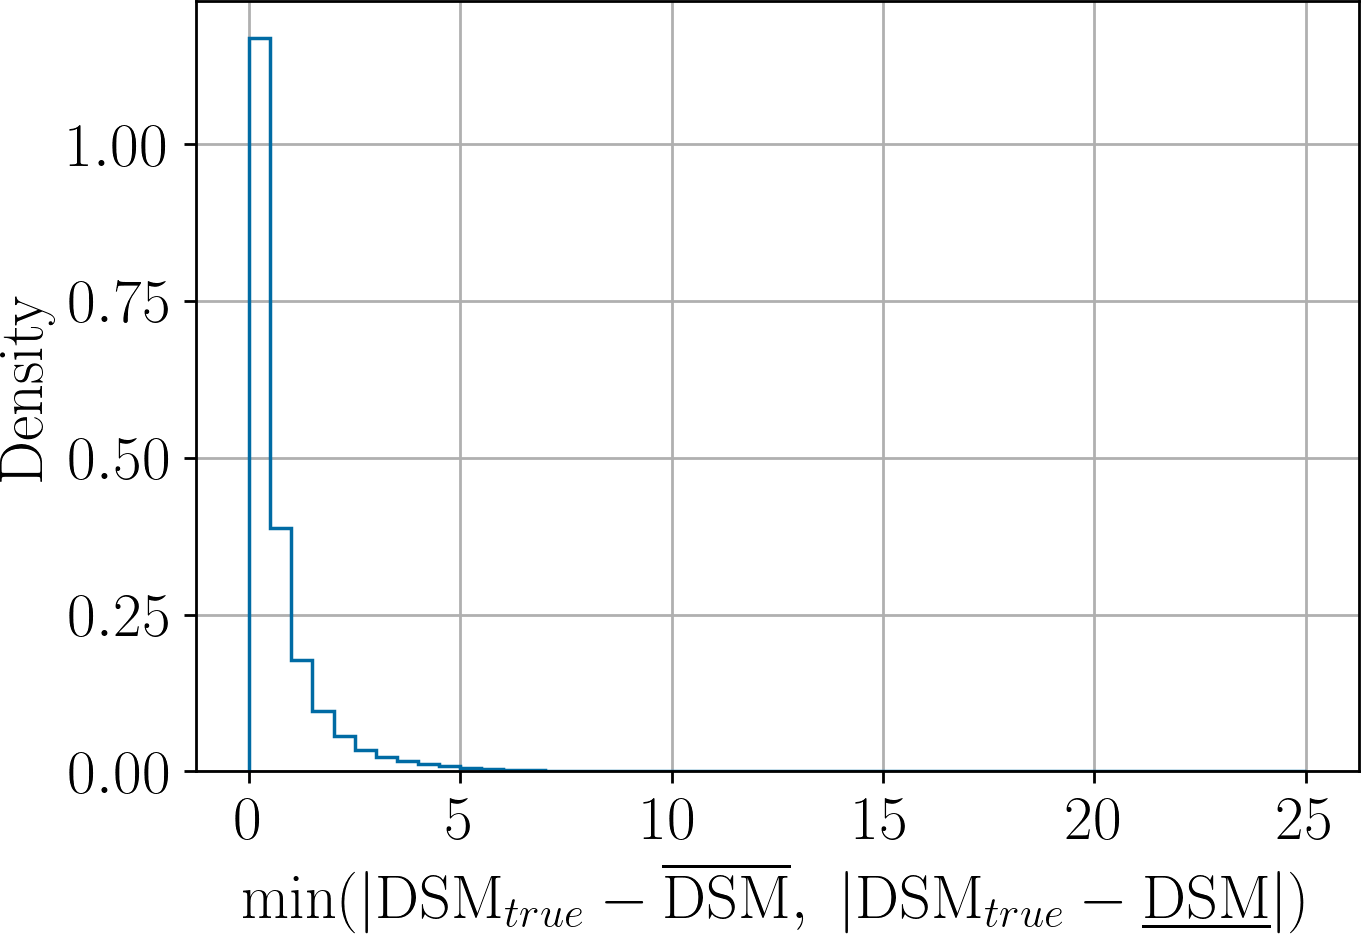
\includegraphics[width=\linewidth]{Images/Chap_6/histogram_elevation_eps_Toulouse.png}
        \caption{Relative errors histogram}\commanue{pourquoi ça dépasse 1 ?}
        \label{fig:error_hist}
    \end{subfigure}\centering
    \begin{subfigure}[t]{0.5\linewidth}
        \flushright
        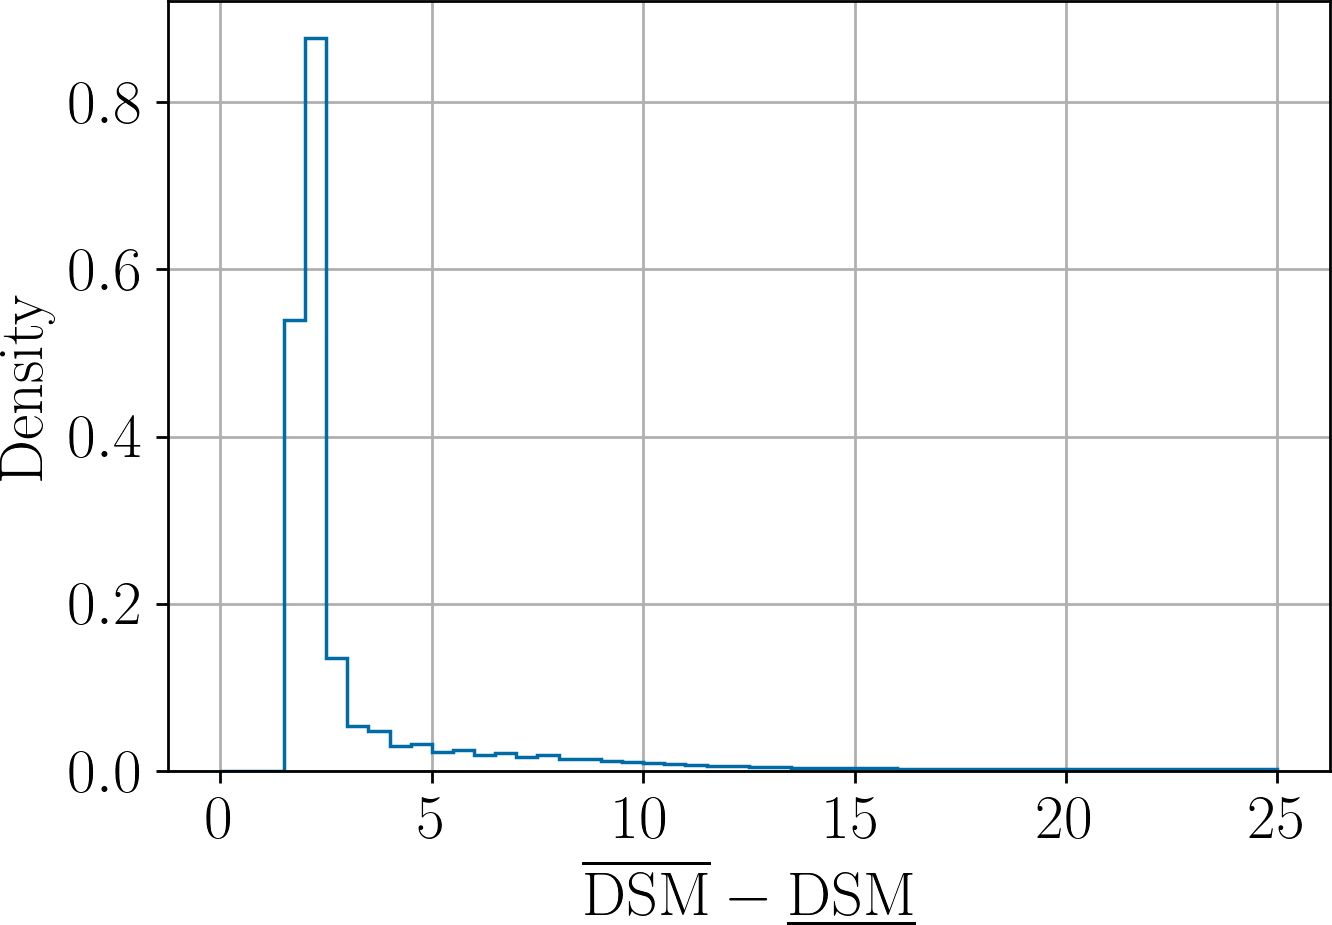
\includegraphics[width=\linewidth]{Images/Chap_6/histogram_elevation_s_rel_Toulouse.png}
        \caption{Relative size histogram}\commanue{en fait je comprends pas les ordonnées sur les graphiques}
        \label{fig:size_hist}
    \end{subfigure}
    \caption{Histograms of the relative error and relative over the Toulouse scene. $Z_{\varepsilon}$ and $Z_{size}$ are defined as the median of those distributions.}
    \label{fig:histogram_elevation_toulouse}
\end{figure}


\begin{comment}
    subsubsection{Relative elevation over-estimation $Z_o$}
    The relative elevation over-estimation $Z_o$, defined in, estimates the proportion of intervals that is superfluous. It seems to be always near $50\%$, which is an acceptable proportion
\end{comment}

\subsection{Altimetric ratio and invalid pixels.}
Looking at \Cref{tab:elevation_metrics_global}, it seems that high values of the altimetric ratio $r_{alt}$ are correlated to low values of accuracy. This is because the convergence angle of satellite is reduced for the acquisition of urban scenes, in order to reduce the proportion of occluded pixels. A low convergence angle results in a high altimetric ratio, as seen in \Cref{fig:incidence_angle}. But it is also harder to correctly reconstruct urban scenes using photogrammetry. The accuracy of intervals is therefore lower in those areas. In short, high values of the altimetric ratio and low accuracy are both linked to urban \acrshort{dsm}, but one does not imply the other and conversely \commanue{A mon avis il faut revoir l'ordre des phrase. Tu notes le constat càd la corrélation. Tu expliques ensuite d'où elle peut provenir et ensuite tu dis que tu observes ce problème plus sur les villes car on réduit le B/H lors des acquisitions pour éviter les occlusions. Là mon problème c'est que j'ai des remarques générales entre des phrases liées à des scènes urbaines donc c'est compliqué de comprendre l'idée que tu veux faire passer. Est-ce que tu veux expliquer qqch de générique qui se voit plus sur l'urbain ou tu veux expliquer qqch de spécifique à l'urbain ?}.

The proportion of invalid pixels that are not considered in the metrics can sometimes be quite high, as it is the case for Monaco (41$\%$) or Hellmem (34.7$\%$). This is due to the presence of water in large part of the image (\Cref{fig:miniature_Monaco_rgb}) or simply the absence of data form the provided ground truth (\Cref{fig:miniature_Hellmem_gt})\commanue{Est-ce qu'il faudrait pas remonter ça comme remarque avant que tu partes une analyse des métriques. La paragraphe d'avant a pour objectif de montrer qu'il y a un lien entre alti ratio et invalid pixels. Mais là c'est encore autre chose.}.


\todoroman{Mettre des images d'erreur et des coupes qui fonctionnent bien}

\section{Comparison with ``naive'' intervals}
The fact that most intervals have a relative size $Z_{size}$ of around 2 pixels may raise the following question: would ``naive'' intervals be accurate ? We define naive intervals $[\underline{\DSM}_{naive}, ~\overline{\DSM}_{naive}]$, as intervals centered on the predicted \acrshort{dsm} with a size of 2 times the altimetric ratio $r_{alt}$:
\begin{align}
    [\underline{\DSM}_{naive}, ~\overline{\DSM}_{naive}] = [\DSM-r_{alt}, \DSM+r_{alt}]
\end{align}
\Cref{tab:naive_accuracy} allows to compare the accuracy of the naive intervals with that of our interval method. The table also contains the mean and median errors of the \acrshort{dsm} defined as:
\begin{align}
    \varepsilon_{\mean} = \mean|\DSM - \DSM_{true}|\qquad \varepsilon_{\median} = \median|\DSM - \DSM_{true}|
\end{align}

\begin{table}[ht]
    \centering
    \begin{tabular}{|c||c|c|c|c|}
        \hline
        Scene & $Z_{acc}$ (pix) & ``Naive'' $Z_{acc}$ (pix) & $\varepsilon_{\median}$ (m) & $\varepsilon_{\mean}$ (m)
        \\\hline\hline
        Bordeaux & 89.3$\%$ & 62.9$\%$ & 0.86 & 1.93\\\hline
        Graasubreen & 99.7$\%$ & 98.8$\%$ & 0.19 & 0.28\\\hline
        Hellmem & 98.8$\%$ & 96.4$\%$ & 0.22 & 0.75\\\hline
        Grenoble & 93.1$\%$ & 65.7$\%$ & 0.61 & 2.08\\\hline
        Langfjordjøkelen & 99.4$\%$ & 88.1$\%$ & 0.26 & 1.31\\\hline
        Monaco & 90.3$\%$ & 61.2$\%$ & 0.69 & 1.75\\\hline
        Montpellier & 89.1$\%$ & 79.4$\%$ & 1.81 & 2.52\\\hline
        Paris & 84.6$\%$ & 82.4$\%$ & 2.35 & 3.59\\\hline
        Peyto & 98.9$\%$ & 95.6$\%$ & 0.32 & 0.56\\\hline
        Pic du midi & 98.1$\%$ & 86.1$\%$ & 0.31 & 1.08\\\hline
        Toulouse & 92.0$\%$ & 83.2$\%$ & 0.92 & 1.79\\\hline
    \end{tabular}
    \caption{Comparison of ``naive'' intervals accuracy with our method for elevation intervals. The median and mean error of the predicted $\DSM$ are also indicated for reference.}
    \label{tab:naive_accuracy}
\end{table}
\Cref{tab:naive_accuracy} indicates that all ``naive'' intervals have a lower accuracy than intervals defined using our method. The difference is sometimes quite substantial, as for the Bordeaux, Grenoble or Monaco scenes where the accuracy drops from around $30\%$ between the two methods. It also corresponds to scenes with a relative elevation size $Z_{size}$ which is higher than on the others scenes. This confirms that our method correctly adapts the size of elevation intervals to each scene individually. It also proves that our method can provide good performance even when the predicted $\DSM$ is far from the ground truth (indicated by high values of $\varepsilon_{\median}$ and $\varepsilon_{\mean}$). 

\section{Influence of Slope on the Metrics}
Using \cref{eq:slope}, it is possible to compute the slope of the scene from the ground truth \acrshort{dsm}. It would be interesting to take a deeper look at the behavior\commanue{alors c'est behaviour en UK et behavior aux US, fais ton choix} of elevation metrics depending on the slope. To do so, we compute the slope $\sigma$\commanue{je sais pas si c'est le meilleur choix de symbole, ça fait un peu trop std deviation.} for each pixel and divided the ranges of slopes in different sections. Those sections are delimited by the following values, from \cite{hugonnet_uncertainty_2022}:
$$
[0\degree, ~2.5\degree, ~5\degree, ~10\degree, ~15\degree, ~20\degree, ~30\degree, ~40\degree, ~50\degree, ~70\degree, ~90\degree]
$$
We then evaluated the metrics on each slope range separately. Results are presented in \Cref{fig:slope_size,fig:slope_eps}. Those figures illustrate the fact that intervals\commanue{elevation intervals} have better performances\commanue{fais attention à ce genre de tournure c'est pas très précis} on low slopes than steep slopes\comloic{pourquoi c'est pas low versus high? Tu mélanges pas la valeur du slope et le caractère de la pente ? Peut être flat et steep alors si tu préfères ?}.

\begin{figure}
    \begin{subfigure}[t]{0.495\linewidth}
        \flushleft
        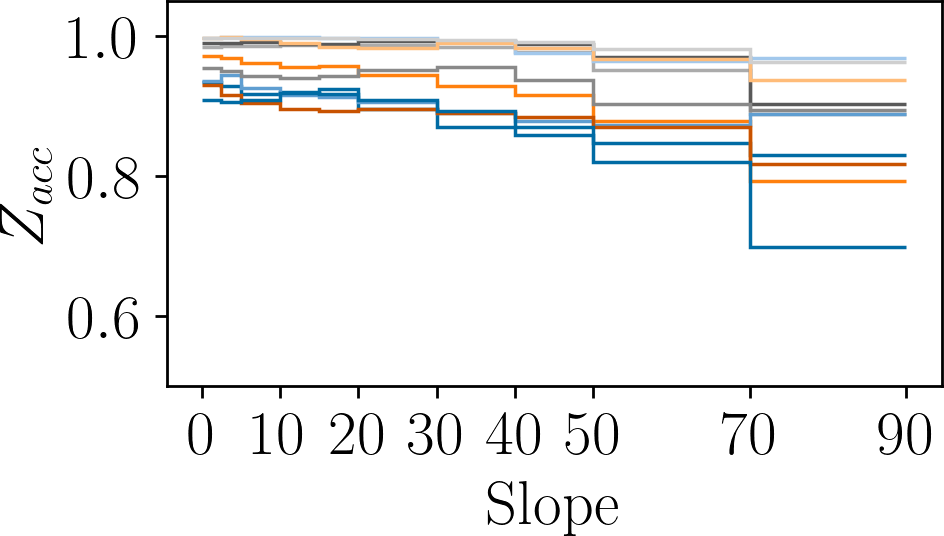
\includegraphics[width=\linewidth]{Images/Chap_6/slope_acc.png}
        \caption{Accuracy $Z_{acc}$}
        \label{fig:slope_acc}
    \end{subfigure}
    \begin{subfigure}[t]{0.495\linewidth}
        \flushright
        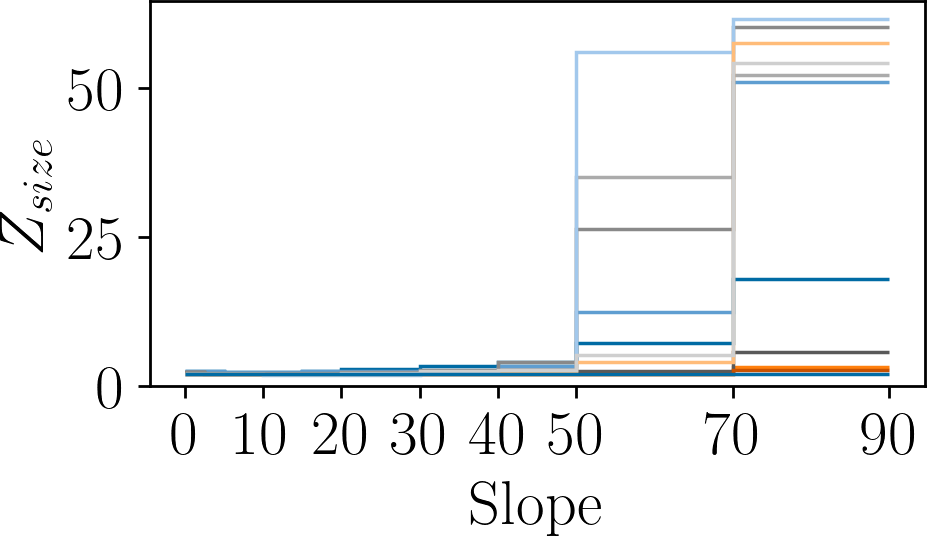
\includegraphics[width=\linewidth]{Images/Chap_6/slope_s_rel.png}
        \caption{Relative size $Z_{size}$}
        \label{fig:slope_size}
    \end{subfigure}
    \caption{Accuracy $Z_{acc}$ and relative size $Z_{size}$ values depending on the slope (in degree). Each curve corresponds to a different scene.}
    \label{fig:slope_acc_size}
\end{figure}

\begin{figure}
    \begin{subfigure}[t]{0.495\linewidth}
        \flushleft
        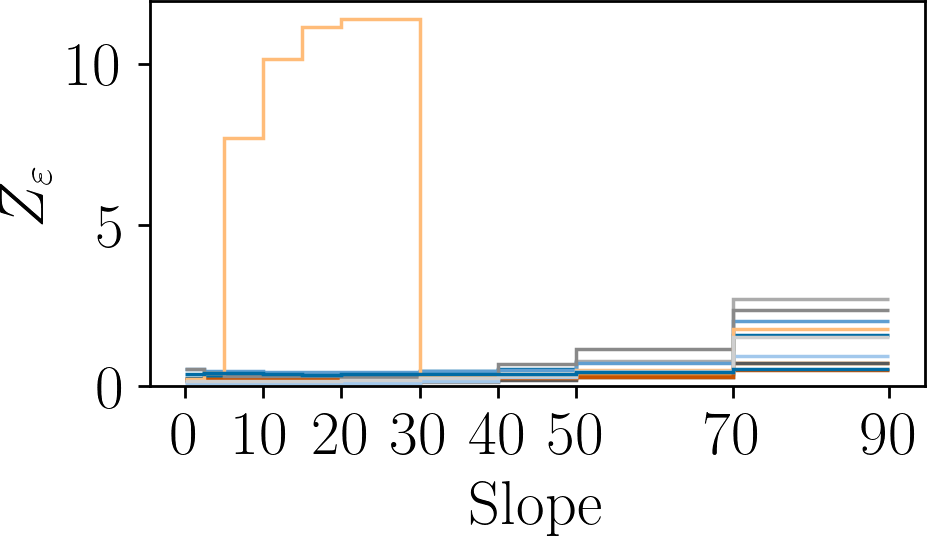
\includegraphics[width=\linewidth]{Images/Chap_6/slope_eps.png}
        \caption{Relative error $Z_\varepsilon$}
        \label{fig:slope_eps_all}
    \end{subfigure}
    \begin{subfigure}[t]{0.495\linewidth}
        \flushright
        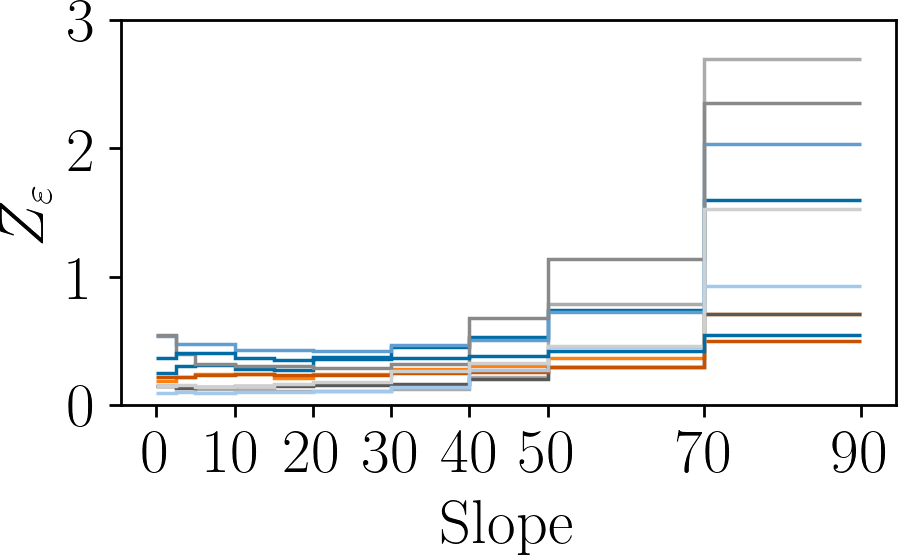
\includegraphics[width=\linewidth]{Images/Chap_6/slope_eps_no_Hellmem.png}
        \caption{Relative error $Z_\varepsilon$ without Hellmem yellow curve}
        \label{fig:slope_eps_no_hellmem}
    \end{subfigure}
    \caption{Relative error $Z_{\varepsilon}$ values depending on the slope (in degree). Each curve corresponds to a different scene. In \Cref{fig:slope_eps_no_hellmem}, we removed the Hellmem yellow curve from \Cref{fig:slope_eps_all} for more visibility.}
    \label{fig:slope_eps}
\end{figure}

Regarding the accuracy of intervals, it tends to drop with sleeper slopes\comloic{sleeper slopes ? vivement la fin de la thèse il te manque un peu de sommeil non ? ;-)}. This can be explained due to a couple of reasons. First, we know that the dense matching correlator performs better\commanue{pareil assez générique comme tournure} on smooth surfaces\comloic{sauf à ce que la smooth surface soit peu texturée et que tu te retrouves avec des zones entières à la mauvaise altitude, ça reste un vote majoritaire en qlq sortes} due to the \acrshort{sgm} regularization which penalizes changes in disparity, and therefore in elevation. The second reason is that intervals are less sensitive to planimetric errors on low slopes than on steep one. This can be visualized on \Cref{fig:Slope_effect_error}\commanue{alors je ne sais pas si c'est l'heure tardive mais je comprends pas ce que tu veux dire et c'est pareil avec le schéma}\comloic{alors là faudra qu'on en reparle... j'ai pas compris et ça m'inquiète parce que je me demande à quel point l'analyse faite sur le slope ne dépend pas aussi de ton angle d'incidence quand même.}. Intervals on steeper slope therefore tend to be less accurate.

\begin{figure}
    \centering
    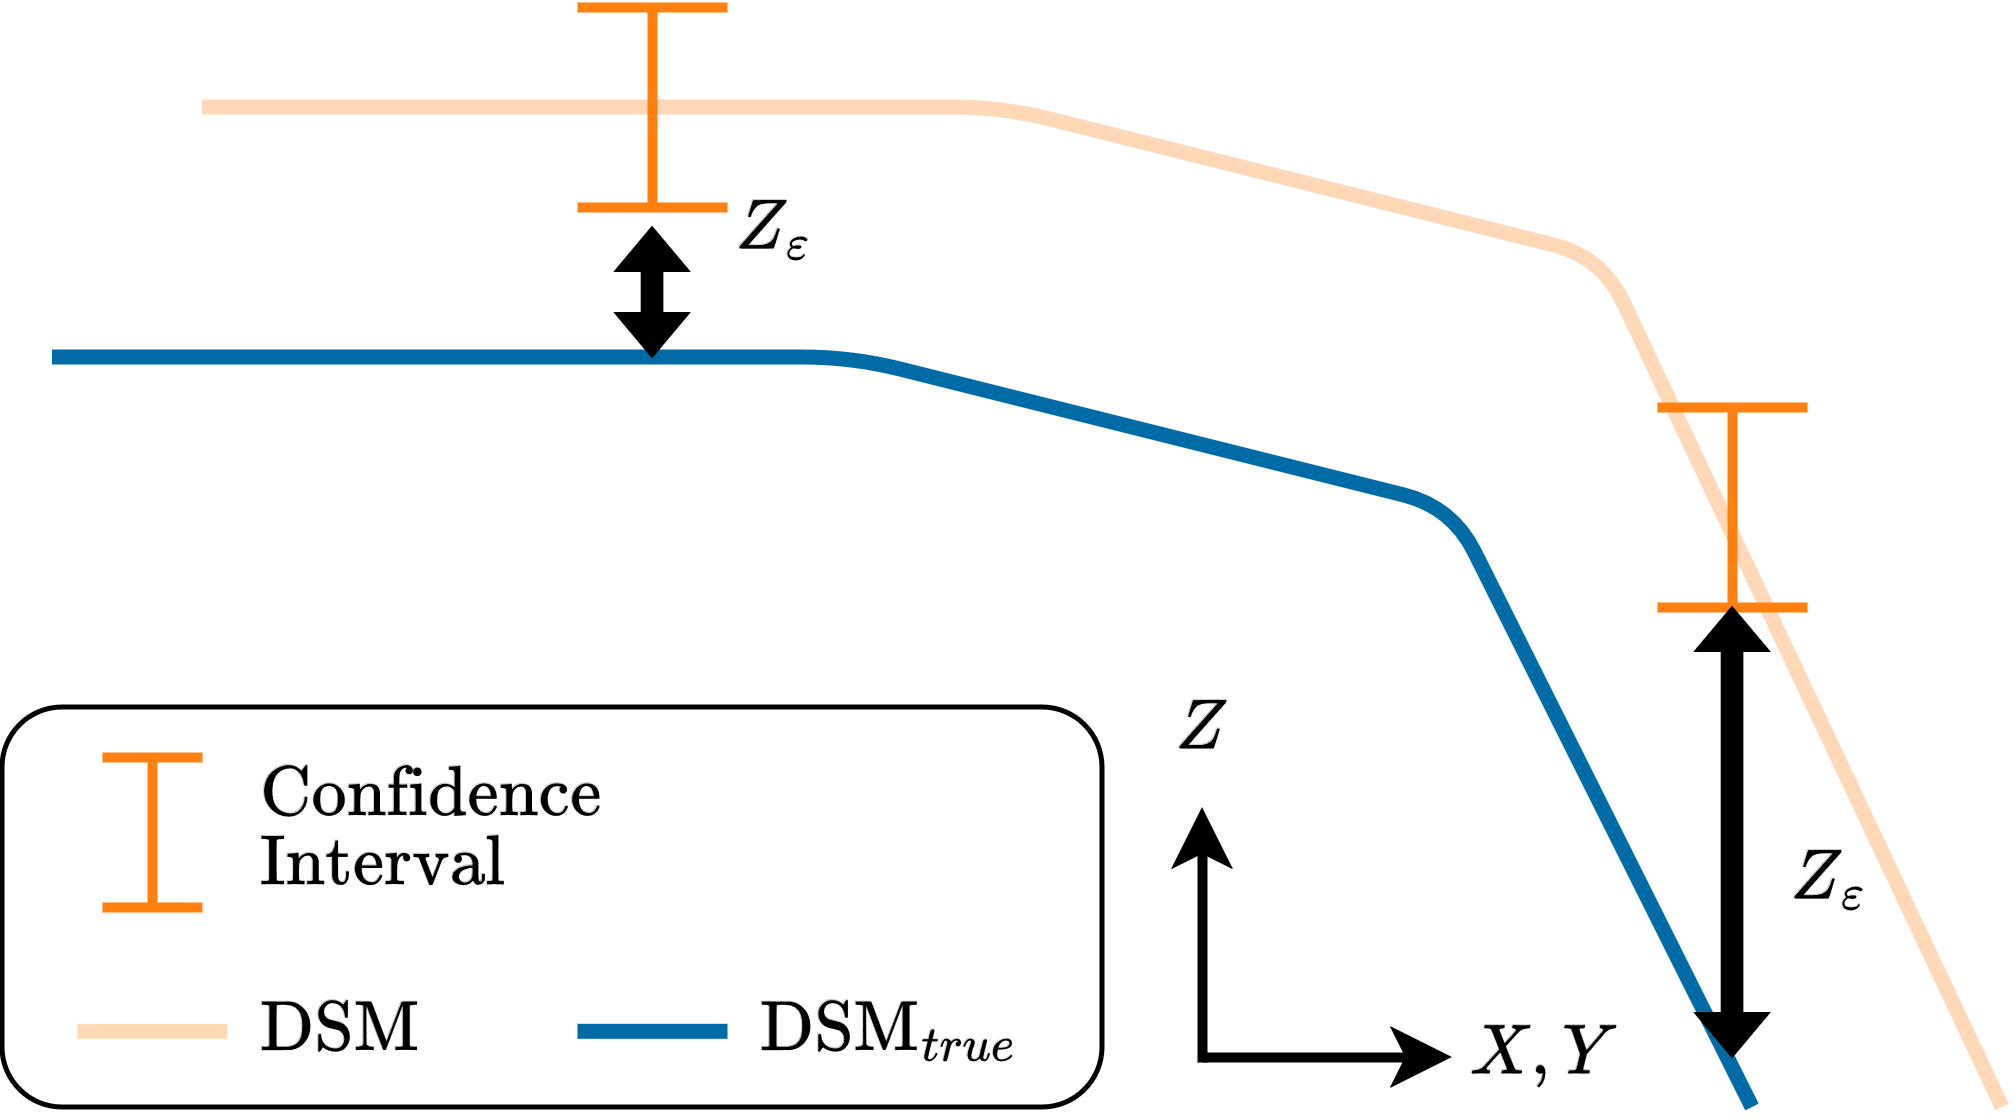
\includegraphics[width=0.7\linewidth]{Images/Chap_6/Slope_effect_error.png}
    \caption{Influence of slope and planimetric error on the accuracy of intervals. The planimetric error does not have an influence on the accuracy of the left interval, while it affects the right interval located on a steeper slope.}
    \label{fig:Slope_effect_error}
\end{figure}

The size of intervals are greater on steep slopes. This is due to the fact that we purposefully detected disparity variations\commanue{est-ce que c'est pas car on est sur des zones ambigues et que l'on a régularisé les intervallles, donc les intervalles sont plus grands sur ces zones?}, and then extended the disparity intervals near those disparity fluctuations. Because disparity changes indicate a variation in elevation, height intervals obtained from disparity intervals are consequently larger on steeper slopes. 

Finally the relative error also increases with slope. This can also be understood using \Cref{fig:Slope_effect_error}, as a steeper slope on the right interval would lead to a greater error\commanue{bah comme je compreds pas lla figure ça m'aide pas}. \Cref{fig:slope_eps_all,fig:slope_eps_no_hellmem} are the same, except we removed one scene, Hellmem, in the right figure. As mentioned earlier, this scene has very few pixels in error, and the median is thus not a robust indicator on this scene.

\section{Other sources of error}\label{sec:other_errors}
We saw in \Cref{sec:results_elevation} that elevation confidence intervals present good results\commanue{Camille te dirait good results c'est vraiment vague. Globalement pour ce chapitre tu utilises bcp de good et better dans l'analyse de tes résultats, c'était moi vrai dans le chapitre 5. Donc essaies d'être précis}, both in accuracy and size. There were however three scenes that did not meet the accuracy objective of $90\%$: Bordeaux, Montpellier and Paris. We will see in this section that there are different factors which can explain why the accuracy objective was not verified on those scenes. Those reasons are: 
\begin{itemize}
    \item Asynchronicity of the ground truth and satellite acquistions
    \item Rasterization of \acrshort{lidar} data over vegetation
    \item Vibrations of the satellite during the images acquistion
\end{itemize}

\subsection{Asynchronicity of sources}
The dates of acquisition of \acrshort{lidar} data and Pléiades images were presented in \Cref{tab:dates_pleiades_lidar_hd}. In some scenes, large periods of time separate the \acrshort{lidar} data from the satellite image, partly because we also tried to minimize the seasonality changes. Specifically, the time between acquisitions for Bordeaux, Grenoble, Monaco and Montpellier ranges between 5 and 13 months. This can lead to major changes of elevation in those scenes. A remarkable example of this can be found on the Monaco scene. If we take a look at the errors on this scene in \Cref{fig:Monaco_errors_global}, we can see that there is a strong concentration of those errors on the top left corner of the image. 

\begin{figure}
    \begin{subfigure}[t]{0.495\linewidth}
        \flushleft
        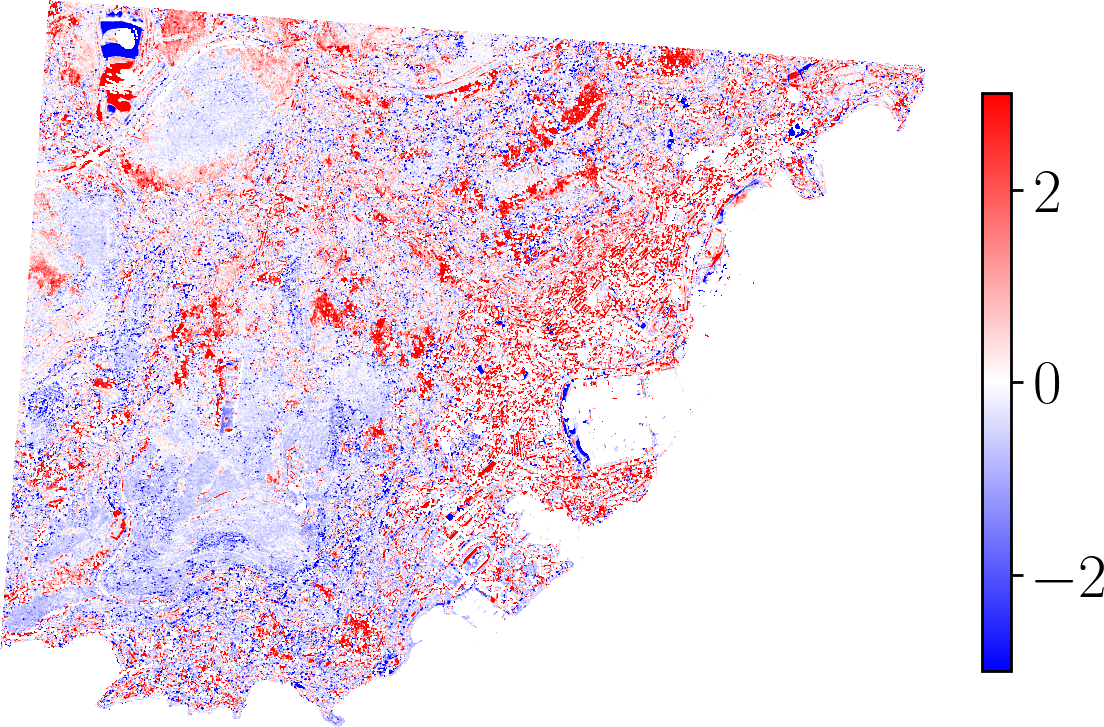
\includegraphics[height=5cm]{Images/Chap_6/Monaco_errors.png}
        \caption{Error $\DSM-\DSM_{true}$}
        \label{fig:Monaco_errors}
    \end{subfigure}
    \begin{subfigure}[t]{0.495\linewidth}
        \flushright
        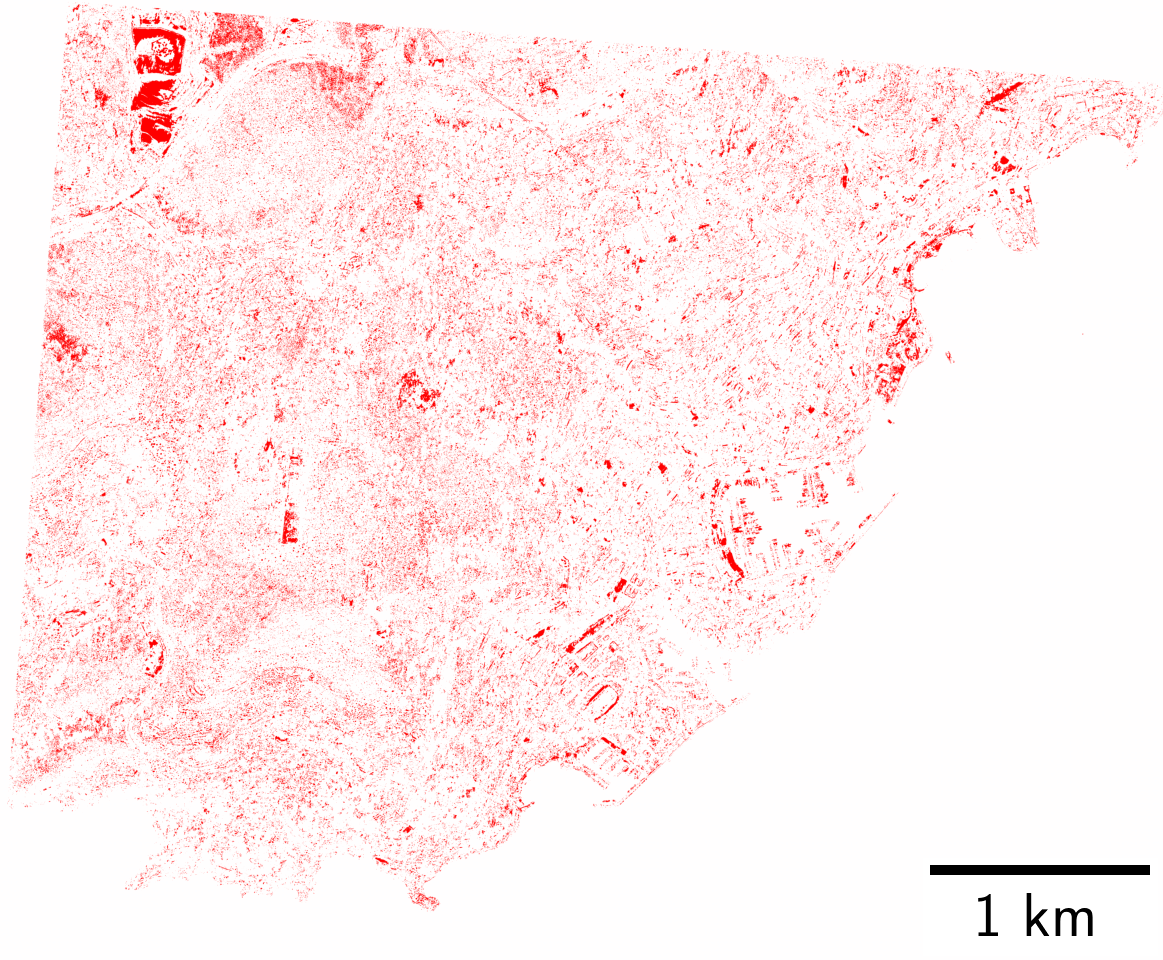
\includegraphics[height=5cm]{Images/Chap_6/Monaco_wrong_intervals.png}
        \caption{Position of wrong intervals, in red.}
        \label{fig:Monaco_wrong_intervals}
    \end{subfigure}
    \caption{Errors and position of wrong intervals on the Monaco scene}
    \label{fig:Monaco_errors_global}
\end{figure}

\Cref{fig:Carriere} is a zoom on this area. By looking at the differences between the \acrshort{rgb} image in \Cref{fig:Carriere_RGB} and the ground truth \acrshort{dsm} in \Cref{fig:Carriere_gt}, we can see that there are some differences between the ground truth and the satellite image (most notably, the bottom left of quarry levels are more constricted on the ground truth that on the \acrshort{rgb} image). We can confidently state that the quarry was excavated some more between the images acquisition and the \acrshort{lidar} acquisition that occurred a year later\commanue{bah là c'est clair}. This explains why so many intervals are wrong in the area, in comparison with the rest of the scene. This can also be observed on a cross section of the \acrshort{dsm}s presented in \Cref{fig:Carriere_row}. Those intervals are thus false negatives, and lower the global accuracy of the scene as they approximately represent around $1.5\%$ of the valid data on this scene.

\begin{figure}
    \begin{subfigure}[t]{0.33\linewidth}
        \flushleft
        \includegraphics[width=\linewidth]{Images/Chap_6/Carriere_gt_Monaco.png}
        \caption{Ground truth DSM. Orange line is detailed in \Cref{fig:Carriere_row}}
        \label{fig:Carriere_gt}
    \end{subfigure}\hfill
    \begin{subfigure}[t]{0.33\linewidth}
        \centering
        \includegraphics[width=\linewidth]{Images/Chap_6/Carriere_RGB_Monaco.png}
        \caption{\acrshort{rgb} image}
        \label{fig:Carriere_RGB}
    \end{subfigure}\hfill
    \begin{subfigure}[t]{0.33\linewidth}
        \flushright
        \includegraphics[width=\linewidth]{Images/Chap_6/Carriere_wrong_intervals_Monaco.png}
        \caption{Position of wrong intervals, in red.}
        \label{fig:Carriere_wrong_intervals}
    \end{subfigure}\\
    \begin{subfigure}[t]{\linewidth}
        \flushright
        \includegraphics[width=\linewidth]{Images/Chap_6/Carriere_row_800.png}
        \caption{\acrshort{dsm}, ground truth and elevation intervals along the orange line of \Cref{fig:Carriere_gt}.}
        \label{fig:Carriere_row}
    \end{subfigure}
    \caption{Detail over the La Turbie quarry, in the top left corner of the Monaco scene.}
    \label{fig:Carriere}
\end{figure}

This type of false negative can be found on a smaller scale in most urban scenes with an asynchronicity of acquisitions\commanue{due to asynchronicity between satellite and lidar acquisitions}. We did not manually detect and correct every building that was destroyed or built in-between acquisitions, as it was too time-consuming. The accuracy results could therefore be further improved on some scenes. It is possible, although very unlikely, that asynchronicity causes false positive during the accuracy computation.

\subsection{LiDAR data over vegetation}\label{eq:lidar_vegetation}
Intervals computed over the Paris scene have an accuracy of $84.6\%$, which is the lowest of all scenes. When trying to understand why the intervals did not seem to perform correctly, we noticed that many pixels in error occurred over trees. This can be observed in \Cref{fig:paris_error_tree}, where many intervals are wrong near trees. By looking at the intervals in \Cref{fig:paris_error_tree_line,fig:Bordeaux_zoom}, we can see that the photogrammetry \acrshort{dsm} over estimates the height of the canopy: columns 4150 to 4170 and 4345 to 4450 of the Paris scene, and columns 3400 to 3800 of the Bordeaux scene. Other buildings and the grounds do not present such error. One probable hypothesis is that because the \acrshort{lidar} HD over Paris was acquired in early March, and the images\commanue{satellite images} in the last day of May, trees foliage had major differences. Firstly, the trees seem bigger on the \acrshort{rgb} image than on the \acrshort{lidar} DSM, which is probably due to a the increase of foliage in-between acquisitions. Also, the \acrshort{lidar} probably acquired points both on the top of trees and on the ground, through the sparse foliage. When rasterizing the \acrshort{lidar} point cloud using a Gaussian mean, we averaged both points on top of the trees and on the ground, resulting in a mix between the two elevations. Due to its resolution, the photogrammetry \acrshort{dsm} does not create multiple points both on the top and at the base of the same tree. It thus only predicts the elevation of the tree top, resulting in the observed error when comparing with \acrshort{lidar} \acrshort{dsm}. We could try to mask the vegetation pixels, using a mask computed from the Normalized Difference Vegetation Index \cite{gao_ndwinormalized_1996}, but the quality of the masks were not good\commanue{sufficiently accurate?}\comloic{je suis un peu perturbé... tu dis "we could try" ce que je traduis par le fait que tu ne vas pas le faire. "We could have tried" et tu aurais pu le faire mais ne l'a pas fait non? Et puis tu dis ensuite que les résultats "were not good" donc en fait tu l'as fait non?} and tend to mask many other pixels that were not vegetation. We therefore chose not to use them. Also, this effect was particularly present on the Paris scene, which is probably because the \acrshort{lidar} was acquired from June to September for the other scenes\commanue{alors précédemment dans le paragraphe, c'est de Mars à Mai donc c'est quoi les dates}, were the vegetation is denser. Furthermore, we will see in the next section that there is a greater source of error occurring on that scene, which probably makes up for most observed errors. 

\begin{figure}
    \centering
    \begin{subfigure}[t]{\linewidth}
        \flushright
        \includegraphics[width=0.95\linewidth]{Images/Chap_6/paris_error_tree_gt.png}
        \caption{Ground truth DSM. Orange line is detailed in \Cref{fig:paris_error_tree_line}}
        \label{fig:paris_error_tree_gt}
    \end{subfigure}\\
    \begin{subfigure}[t]{\linewidth}
        \flushright
        \includegraphics[width=0.95\linewidth]{Images/Chap_6/paris_error_tree_clr.png}
        \caption{\acrshort{rgb} image}
        \label{fig:paris_error_tree_clr}
    \end{subfigure}\\
    \begin{subfigure}[t]{\linewidth}
        \flushright
        \includegraphics[width=0.95\linewidth]{Images/Chap_6/paris_error_tree_intervals.png}
        \caption{Position of wrong intervals, in red.}
        \label{fig:paris_error_tree_intervals}
    \end{subfigure}\\
    \begin{subfigure}[t]{\linewidth}
        \centering
        \includegraphics[width=\linewidth]{Images/Chap_6/paris_error_tree.png}
        \caption{\acrshort{dsm}, ground truth and elevation intervals along the orange line of \Cref{fig:paris_error_tree_gt}}
        \label{fig:paris_error_tree_line}
    \end{subfigure}
    \caption{Zoom near Saint-Augustin, in the Paris scene}
    \label{fig:paris_error_tree}
\end{figure}

\begin{figure}
    \begin{subfigure}[t]{0.33\linewidth}
        \flushleft
        \includegraphics[width=\linewidth]{Images/Chap_6/Bordeaux_gt_zoom.png}
        \caption{Ground truth DSM. Orange line is detailed in \Cref{fig:Bordeaux_row}}
        \label{fig:Bordeaux_gt}
    \end{subfigure}\hfill
    \begin{subfigure}[t]{0.33\linewidth}
        \centering
        \includegraphics[width=\linewidth]{Images/Chap_6/Bordeaux_clr_zoom.png}
        \caption{\acrshort{rgb} image}
        \label{fig:Bordeaux_RGB}
    \end{subfigure}\hfill
    \begin{subfigure}[t]{0.33\linewidth}
        \flushright
        \includegraphics[width=\linewidth]{Images/Chap_6/Bordeaux_error_zoom.png}
        \caption{Position of wrong intervals, in red.}
        \label{fig:Bordeaux_wrong_intervals}
    \end{subfigure}\\
    \begin{subfigure}[t]{\linewidth}
        \flushright
        \includegraphics[width=\linewidth]{Images/Chap_6/Bordeaux_row_600.png}
        \caption{\acrshort{dsm}, ground truth and elevation intervals along the orange line of \Cref{fig:Bordeaux_gt}.}
        \label{fig:Bordeaux_row}
    \end{subfigure}
    \caption{Detail over the Quinconces square, in the the Monaco scene.}
    \label{fig:Bordeaux_zoom}
\end{figure}


\subsection{Vibration of the satellite}\label{sec:vibrations}
The previous sources of errors concerned the quality of the ground truth \acrshort{dsm}. However, there is one source of errors that we did not take into consideration in our methods: the vibration of the satellites\commanue{satellite vibration during acquisition?}. During the acquisition of images, push-broom captors may experience vibrations which are not modeled in the \acrshort{rpc} model\commanue{je ne sais pas si tu as un schéma avec les angles roulis, tangage, lacet du satellite mais ce sera bien pour expliquer quel angle vibre}. This translates into low frequency along-track biases on the \acrshort{dsm}, sometimes called undulations \cite{hugonnet_uncertainty_2022}. This can be detected by looking at the difference between the photogrammetry and the ground truth \acrshort{dsm}s:
\begin{align}
    \DSM(\rowcol)-\DSM_{true}(\rowcol)
\end{align}
Without biases, this difference (or relative error), should not be correlated with the position $\rowcol$ in the image. \Cref{fig:vibrations} presents all scenes for which we detected a bias. The bias is small on \Cref{fig:vibrations_Hellmem} but is hard to miss on \Cref{fig:vibrations_Montpellier,fig:vibrations_Paris,fig:vibrations_Toulouse}. \Cref{fig:vibration_bias} indicates that those biases can reach 2.5m of amplitude.

\begin{figure}
    \begin{subfigure}[t]{0.48\linewidth}
        \flushleft
        \includegraphics[width=\linewidth]{Images/Chap_6/vibrations_Hellmem.png}
        \caption{Hellmem}
        \label{fig:vibrations_Hellmem}
    \end{subfigure}\hfill
    \begin{subfigure}[t]{0.48\linewidth}
        \flushright
        \includegraphics[width=\linewidth]{Images/Chap_6/vibrations_Montpellier.png}
        \caption{Montpellier}
        \label{fig:vibrations_Montpellier}
    \end{subfigure}\\
    \begin{subfigure}[t]{0.48\linewidth}
        \flushleft
        \includegraphics[width=\linewidth]{Images/Chap_6/vibrations_Paris.png}
        \caption{Paris}
        \label{fig:vibrations_Paris}
    \end{subfigure}\hfill
    \begin{subfigure}[t]{0.48\linewidth}
        \flushright
        \includegraphics[width=\linewidth]{Images/Chap_6/vibrations_Toulouse.png}
        \caption{Toulouse}
        \label{fig:vibrations_Toulouse}
    \end{subfigure}
    \caption{Difference $(\DSM-\DSM_{true})$ for different scenes. A bias along rows (along-track) appears, suggesting vibrations during the image acquisition. Biases on the Hellmem \acrshort{dsm} are smaller that for the other three scenes.}
    \label{fig:vibrations}
\end{figure}

When computing confidence elevation intervals, we did not consider potential errors of this magnitude stemming from the \acrshort{rpc} models. Our method principally aimed to model and propagate the errors stemming from the dense matching step, which we considered to be the part of the pipeline where largest errors could occur. Biases observed in \Cref{fig:vibrations} indicate that only considering the dense matching errors is not sufficient when producing \acrshort{dsm}s with Pléiades images. However, the CO3D satellites will not use a push-broom sensor, but rather a CCD Bayer matrix, which will circumvent any vibration issue\commanue{alors de là à dire que tu n'auras pas de problème de vibration, c'est un peu fort tu as quand même un satellite qui défile et qui doit modifier son orientation pour rester suffisamment longtemps sur la zone à imager. Mais peut-être pas en tangage}\comloic{grave ! je te propose d'en parler à Fabrice je pense qu'il va te faire modérer ton langage ;-)}.

In the scope of this thesis, we did not try to model the uncertainty associated with potential vibrations of the satellite. It would however be interesting to determine if Montpellier and Paris scenes could validate the $90\%$ accuracy objective without the effect of the vibrations. We therefore propose a simple correction of the vibration effect, which is not meant to perfectly solve the issue but rather to sufficiently reduce it for a better evaluation of the elevation interval metrics. In order to do so, we computed the residual error $(\DSM-\DSM_{true})$, and attempted to model the observed bias using a least square approach. We suppose that the bias depends only on the row of the image and propose to simply model it by a cosine function carried by a linear function of the row:
\begin{align}\label{eq:bias_model}
    bias(row)=A_1\cos(A_2\cdot row+A_3) + A_4\cdot row+A_5
\end{align}
where $(A_1\enum A_5)$ are the parameters of our model. \Cref{fig:vibration_bias} shows scatter plots of the residual error $(\DSM-\DSM_{true})$ where the x-axis indicates image rows. We also computed the median of the residual error for each row as an indicator of the distribution of errors, and the optimized model from \cref{eq:bias_model}.

\begin{figure}
    \begin{subfigure}[t]{\linewidth}
        \centering
        \includegraphics[width=\linewidth]{Images/Chap_6/vibration_bias_Montpellier.png}
        \caption{Montpellier scene}
        \label{fig:vibration_bias_Montpellier}
    \end{subfigure}
    \begin{subfigure}[t]{\linewidth}
        \centering
        \includegraphics[width=\linewidth]{Images/Chap_6/vibration_bias_Paris.png}
        \caption{Paris scene}
        \label{fig:vibration_bias_Paris}
    \end{subfigure}
    \caption{Scatter plot where gray points are the residual error $(\DSM-\DSM_{true})$ of a pixel. The x-axis represents the row of each pixel. As an indicator, we also computed the median residual error for each row, appearing in orange. The blue line is the optimized model from \cref{eq:bias_model}.}
    \label{fig:vibration_bias}
\end{figure}

\begin{figure}
    \begin{subfigure}[t]{0.48\linewidth}
        \flushleft
        \includegraphics[width=\linewidth]{Images/Chap_6/vibrations_Montpellier.png}
        \caption{Residual error with bias}
        \label{fig:vibrations_Montpellier_with_bias}
    \end{subfigure}\hfill
    \begin{subfigure}[t]{0.48\linewidth}
        \flushright
        \includegraphics[width=\linewidth]{Images/Chap_6/vibration_corrected_Montpellier.png}
        \caption{Residual error without bias}
        \label{fig:vibrations_Montpellier_without_bias}
    \end{subfigure}
    \caption{Residual error $(\DSM-\DSM_{true})$ with and without the bias estimated in \Cref{fig:vibration_bias} for the Montpellier scene.}
    \label{fig:removed_bias_Montpellier}
\end{figure}

\begin{figure}
    \begin{subfigure}[t]{0.48\linewidth}
        \flushleft
        \includegraphics[width=\linewidth]{Images/Chap_6/vibrations_Paris.png}
        \caption{Residual error with bias}
        \label{fig:vibrations_Paris_with_bias}
    \end{subfigure}\hfill
    \begin{subfigure}[t]{0.48\linewidth}
        \flushright
        \includegraphics[width=\linewidth]{Images/Chap_6/vibration_corrected_Paris.png}
        \caption{Residual error without bias}
        \label{fig:vibrations_Paris_without_bias}
    \end{subfigure}
    \caption{Residual error $(\DSM-\DSM_{true})$ with and without the bias estimated in \Cref{fig:vibration_bias}, for the Paris scene.}
    \label{fig:removed_bias_Paris}
\end{figure}


Having estimated the bias, we can subtract it from the \acrshort{dsm} and its confidence intervals. This will not change the relative size of the intervals are we apply the same elevation shift to both bounds. The accuracy and relative error are however impacted by this bias rectification. Here are the improvements:
\begin{itemize}
    \item For the Montpellier scene, the accuracy $Z_{acc}$ increases $89.1\%$ to $92.6\%$. The relative error $Z_\varepsilon$ also increases from $0.28$ pixels to $0.32\%$ pixels\commanue{c'est normal que tu parles en pixel puis en poucentage de pixels}.
    \item For the Paris scene, the accuracy $Z_{acc}$ increases $84.6\%$ to $88.1\%$. The relative error $Z_\varepsilon$ also increases from $0.18$ pixels to $0.43\%$ pixels\commanue{même remarque}.  
\end{itemize}
The fact that the relative error is slightly larger is probably due to the fact that as the accuracy increases, the set on which $Z_\varepsilon$ is computed gets smaller, and only larger error remains. 

\begin{remark}
    In this section, we used the ground truth to correct the bias from the vibrations of the satellite. We used the ground truth because our objective was to verify if the biases were indeed the source of the missing accuracy of elevation intervals, so that we could safely assume our methods was efficient, granted that no vibrations occurred during the acquisition. 
    
    Our aim was not to propose a general method for modeling or correcting the errors due to vibrations, in which case we could not have used the ground truth as it not available everywhere. However, if such were our intents, using a low resolution \acrshort{dsm} such as the Copernicus \acrshort{dsm} at 30m resolution could suffice to detect the presence of vibrations. This \acrshort{dsm} was already used in the \acrshort{cars} pipeline as our initial elevation. By plotting the differences between the low resolution \acrshort{dsm} and the predicted photogrammetry \acrshort{dsm}, we can indeed observe the presence of vibrations as seen in the following figure:
    
    {\centering\includegraphics[width=7cm]{Images/Chap_6/copernicus_bias_Montpellier.png}
    \captionof{figure}{Difference $\DSM-\DSM_{low}$ between the photogrammetry model $\DSM$ and the low resolution model $\DSM_{low}$ over the Montpellier scene.}}
\end{remark}


The Paris scene still does not reach the $90\%$ accuracy objective, while being very close to it. Looking at \Cref{fig:vibrations_Paris_without_bias}, there still seem to be a bias, horizontally this time, as residuals are positive in the left of the image and negative in the right of the image. We can also distinguish that streets seem to have more positive residuals, which is once again probably due to the vegetation issue discussed in \Cref{eq:lidar_vegetation}. As the accuracy is very close to the $90\%$ objective, and we have good reasons to think there are false negative in our test, we consider that this scene confirms the good performances of our method for creating elevation confidence intervals. 

\section{Unexplored leads}\label{sec:unexplored_leads}
\todoroman{A mettre dans la conclusion plutôt ? Parler du marriage problème à ce moment aussi ?}
In the previous sections, we evaluated the performance of the elevation intervals associated to their respective \acrshort{dsm}s. Those intervals were obtained by triangulation of disparity intervals, to obtain an interval along a line of sight, which was then rasterized. As they stand, intervals are a reflection of the potential error committed during the dense matching step. During our investigations, we came up with other interesting ideas that we did not have time to get to the bottom of. In order to conclude this chapter, we will quickly go over them.

We saw \Cref{fig:toulouse_zoom_row,fig:Carriere_row,fig:Bordeaux_row} that elevation intervals could sometimes reach very high values, like $80$m in the case of Toulouse for instance. Having those intervals means that the bounds of those intervals have a high possibility degree, and that the difference between choosing one bound or the other is not obvious. It could be wise to filter out the 3D points leading to such large intervals. After all, a large elevation interval suggests that we are not certain about the position of the point, so removing it seems natural. Additionally, we ignored the planimetric error $\Delta XY$ during the rasterization as presented in \Cref{fig:planimetric_shift}, but the hypothesis that $\Delta XY$ is small is probably not valid for large intervals. For acquisitions with incidence angles, around 11$\degree$, an elevation interval of 50m would mean that the planimetric uncertainty is around $50\tan(11\degree)\approx20$m. For the Peyto scene, were the incidence is $21.3\degree$, this uncertainty reaches $46$m. Not only are we unsure about the elevation of the point, but there is much uncertainty regarding which cell it falls into during the rasterization process. We can either filter those points directly after the dense matching step, based on the size of the intervals, or after they have been triangulated, based on the resulting planimetric/altimetric shift. The latter allows to also consider the acquisition conditions of images, which may be more adapted to photogrammetry\commanue{je comprends pas la fin de la phrase}.

When triangulating the disparity, we consider line of sights to be 3D lines. However, they represent the position of a pixel, which is not a point but a surface (determined by the resolution of images). Lines of sights are therefore not exactly lines, but rather a cone or a cylinder.  We could even go further with this model, by taking into consideration the accuracy of lines of sights into the definition of those cylinders. Intersecting ``cylinders'' of sights would then yield a 3D volume. We would then have to processed differently the obtained volumes during the rasterization step. 

The rasterization step uses a Gaussian mean based on the distance of 3D points to the center of a cell. We could additionally use the size of intervals to adapt the weights in the rasterization steps. Doing so, we would favor points with small intervals, \ie for which we are confident about their position, to improve the final \acrshort{dsm}. If we reason with 3D volumes, we could compute a density on each volume and project those density on the final raster \etc\commanue{comme d'hab je mettrais pas etc}. 

In any case, we could use the uncertainty information contained in the different intervals (disparity, elevation) to improve the final \acrshort{dsm}\commanue{cette phrase est générique c'est l'objectif de ce que tu proposes précédemment ? Peut-être à mettre en intro en distant que tu distingues les piste qui sont l'amélioration de la définition de l'intervalle des pistes qui sont l'utilisation des intervalles directement dans CARS pour améliorer le pipeline}. As it stands, the computation of intervals does not modify the final \acrshort{dsm}.

In this final chapter, we propagated the uncertainty\commanue{disparity uncertainty} estimated from \Cref{chap:epistemic_uncertainty} as intervals\commanue{elevation intervals} to the end of the photogrammetry pipeline. The intervals represent the uncertainty due to the dense matching step\commanue{fais attention tu as des intervalles sur la disparité et sur l'élévation et c'est pareil pour les incertitudes donc il faut éviter d'être trop flou dans tes phrases}, which is the more complex part of the pipeline, and therefore the most important source of uncertainty. Intervals have an accuracy of $90\%$, and their size is proportionate to the potential errors between the predicted \acrshort{dsm} and the true elevation. Intervals have better performances\commanue{en terme de quoi soit un peu plus précis} on natural landscape than on urban ones, as those scenes contain more elevation differences and greater slopes. Elevation confidence intervals\commanue{ta méthodologie pour calculer les intervalles plutôt} aim to satisfy requirements expressed by \acrshort{dsm} users. They can also provide a good solution for the future CO3D mission requirements, as a performance map will need to be provided alongside the \acrshort{dsm}.

\pagebreak
\blankpage